\documentclass[12pt]{book}
% !TEX root = hazy2.tex
%\includeonly{limits}
%\includeonly{coninter}
%\includeonly{lineatomparam}
%\includeonly{linedetl}
%\includeonly{codestruc}
%\includeonly{CloudyStandaloneProgram}
%\includeonly{sub}
%\includeonly{output}
%\includeonly{observed}
%\includeonly{lines}
%\includeonly{problems}
%\includeonly{odetail}
%\includeonly{sources}
%\includeonly{glossary}
%\includeonly{conversion}
%\includeonly{TestSuite}
%\includeonly{refer}

\usepackage{graphicx,rotate,url,mathptmx,lscape,times,framed,color}

% include natbib for bibtex, options are
% round use (2008) instead of [2008] for year
\usepackage[round]{natbib}

% cross references across documents
\usepackage{xr}

%\begin{comment}
%This is my comment.
%Note that it can span multiple lines.
%This is very useful.
%\end{comment}
\usepackage{verbatim} 

% allow hyperlinks
\usepackage{hyperref}
\hypersetup{
    bookmarks=true,         % show bookmarks bar?
    unicode=false,          % non-Latin characters in Acrobat�s bookmarks
    pdftoolbar=true,        % show Acrobat�s toolbar?
    pdfmenubar=true,        % show Acrobat�s menu?
    pdffitwindow=true,      % page fit to window when opened
    pdftitle={My title},    % title
    pdfauthor={Author},     % author
    pdfsubject={Subject},   % subject of the document
    pdfnewwindow=true,      % links in new window
    pdfkeywords={keywords}, % list of keywords
    colorlinks=true,        % false: boxed links; true: colored links
    linkcolor=blue,         % color of internal links, def red
    citecolor=blue,         % color of links to bibliography, def green
    filecolor=blue,         % color of file links, def magenta
    urlcolor=blue           % color of external links, def cyan
}

% geometry package controls page layout
\usepackage[letterpaper,
left=2.5cm,right=2.5cm,
top=2.5cm,bottom=2.5cm]{geometry}
\oddsidemargin=+0.7cm
\evensidemargin=-0.7cm
\pagestyle{headings}

% journal name macros used by ADS
\usepackage{../common/aas_macros}

% Include list of figures and references in contents lists
\usepackage[nottoc]{tocbibind}

% makes it easy to include all or part of a PDF document 
% inside a LaTeX document
\usepackage{pdfpages}

% allow external files to be included verbatim
\usepackage{moreverb}
% set the default tabsize
\def\verbatimtabsize{4\relax}

% following are to pick up .aux files for cross references
% with package xr to other volumes of Hazy
% hazy 1
\externaldocument[Hazy1-]{../hazy1/intro}
\externaldocument[Hazy1-]{../hazy1/define}
\externaldocument[Hazy1-]{../hazy1/cmdintro}
\externaldocument[Hazy1-]{../hazy1/cont-def}
\externaldocument[Hazy1-]{../hazy1/cont-lum}
\externaldocument[Hazy1-]{../hazy1/cont-shp}
\externaldocument[Hazy1-]{../hazy1/compos}
\externaldocument[Hazy1-]{../hazy1/density}
\externaldocument[Hazy1-]{../hazy1/geometry}
\externaldocument[Hazy1-]{../hazy1/optdepth}
\externaldocument[Hazy1-]{../hazy1/therm}
\externaldocument[Hazy1-]{../hazy1/dynamics-time}
\externaldocument[Hazy1-]{../hazy1/stopping}
\externaldocument[Hazy1-]{../hazy1/conout}
\externaldocument[Hazy1-]{../hazy1/optimize}
\externaldocument[Hazy1-]{../hazy1/grid}
\externaldocument[Hazy1-]{../hazy1/miscell}
\externaldocument[Hazy1-]{../hazy1/latex_style}

% hazy2
\externaldocument[Hazy2-]{../hazy2/limits}
\externaldocument[Hazy2-]{../hazy2/coninter}
\externaldocument[Hazy2-]{../hazy2/lineatomparam}
\externaldocument[Hazy2-]{../hazy2/linedetl}
\externaldocument[Hazy2-]{../hazy2/CloudyStandaloneProgram}
\externaldocument[Hazy2-]{../hazy2/sub}
\externaldocument[Hazy2-]{../hazy2/output}
\externaldocument[Hazy2-]{../hazy2/observed}
\externaldocument[Hazy2-]{../hazy2/lines}
\externaldocument[Hazy2-]{../hazy2/problems}
\externaldocument[Hazy2-]{../hazy2/odetail}
\externaldocument[Hazy2-]{../hazy2/sources}
\externaldocument[Hazy2-]{../hazy2/glossary}
\externaldocument[Hazy2-]{../hazy2/conversion}
\externaldocument[Hazy2-]{../hazy2/TestSuite}

% hazy 3
\externaldocument[Hazy3-]{../hazy3/isoseq}
\externaldocument[Hazy3-]{../hazy3/hydroiso}
\externaldocument[Hazy3-]{../hazy3/helikeiso}
\externaldocument[Hazy3-]{../hazy3/molecules}
\externaldocument[Hazy3-]{../hazy3/dheavy}
\externaldocument[Hazy3-]{../hazy3/dtherm}
\externaldocument[Hazy3-]{../hazy3/dgrain}
\externaldocument[Hazy3-]{../hazy3/dother}

% set paragraph styles
\raggedright
\setlength{\parindent}{4mm}
% background color for shaded boxes
\definecolor{shadecolor}{gray}{0.9}

% Customize contents details from book.cls
\makeatletter

\renewcommand*\l@section{\@dottedtocline{1}{1.5em}{3.1em}}
\renewcommand*\l@subsection{\@dottedtocline{2}{4.6em}{4.1em}}
\renewcommand*\l@subsubsection{\@dottedtocline{3}{8.7em}{5.1em}}
\renewcommand*\l@paragraph{\@dottedtocline{4}{10em}{6em}}
\renewcommand*\l@subparagraph{\@dottedtocline{5}{12em}{7em}}
\renewcommand*\l@figure{\@dottedtocline{1}{1.5em}{3.3em}}

% extract name of target of reference (e.g. chapter titles)
\long\def\@thirdoffive#1#2#3#4#5{#3}%
\def\refname#1{\expandafter\@setref\csname r@#1\endcsname\@thirdoffive{#1}}

% create ruler underneath page header
\advance\headheight1.2pt
\def\@oddhead{\vbox{\parindent=0pt%
\setbox0=\hbox to\textwidth{{\slshape\rightmark}\hfil\thepage}%
\dimen0=4.5pt \advance\dimen0 by-\dp0 \box0\kern\dimen0\hrule}}
\def\@evenhead{\vbox{\parindent=0pt%
\setbox0=\hbox to\textwidth{\thepage\hfil\slshape\leftmark}%
\dimen0=4.5pt \advance\dimen0 by-\dp0 \box0\kern\dimen0\hrule}}

% modify font size for verbatim environment
\newcommand{\setverbatimfontsize}[1]{\renewcommand*\verbatim@font{#1\ttfamily}}
\renewcommand*\verbatim@font{\footnotesize\ttfamily}

% Change title of bibliography
\renewcommand\bibname{REFERENCES}
\renewcommand\contentsname{CONTENTS}
\renewcommand\listfigurename{LIST OF FIGURES}
\renewcommand\listtablename{LIST OF TABLES}
% tweak bibliograpy environment to be more like old Hazy
\def\thebibliography#1{%
\bibsection
\@mkboth{\MakeUppercase\bibname}{\MakeUppercase\bibname}%
\list{}{\setlength\labelwidth{2.5em}\leftmargin\labelwidth
\setlength\parsep{0pt}\setlength\itemsep{0.7mm plus1pt}
\setlength{\itemindent}{-\leftmargin}
\small}
\def\newblock{\hskip .11em plus .33em minus -.07em}
\sloppy
\sfcode`\.=1000\relax}
\def\endthebibliography{\endlist}

\makeatother
% End of contents customization

% some names we use
\newcommand{\Cloudy}{\textsc{Cloudy}}
\newcommand{\Hazy}{\textsc{Hazy}}
\newcommand{\cdCommand}[1]{\textbf{#1}}
\newcommand{\cdVariable}[1]{\emph{#1}}
\newcommand{\cdSectionTitle}[1]{\emph{#1}}
\newcommand{\cdFilename}[1]{\texttt{#1}}
\newcommand{\cdRoutine}[1]{\emph{#1}}
\newcommand{\cdTerm}[1]{\textbf{\emph{#1}}}
\newcommand{\cdMono}[1]{\texttt{#1}}
\newcommand{\fixit}[1]{\textbf{FIXIT: #1}}
\font\manual=manfnt at 7pt \def\dbend{\hbox{\raise0.9ex\hbox{\manual\char127\hspace{0.6em}}}}
\newcommand{\experimental}{\texorpdfstring{\dbend}{??}}

% or symbol provided by Will H
\newcommand\OR{\texorpdfstring{\ensuremath{\vert}}{|}}

% Matt's 1.23\e{-2} 
\providecommand{\e}[1]{\ensuremath{\times 10^{#1}}}


% \ion from Will, replace AAS version
\newcommand\Ion[2]{\ensuremath{\mathrm{#1\,\scriptstyle #2}}}

% macro sometimes found in ADS bibtex entries
\newcommand{\mdash}{---} 

% ion is in the aas style
\newcounter{INTERNALionstage}
\providecommand{\ion}[2]{% replace the aastex version
  \setcounter{INTERNALionstage}{#2}%
  \Ion{#1}{\Roman{INTERNALionstage}}}

\providecommand{\red}[1]{{\color{red}#1}}

% Will's todo and done macros
%\newcommand\TODO[1]{\textbf{\boldmath [#1]}}
\newcommand{\TODO}[1]{\textcolor{red}{{\textbf{\boldmath [#1]}}}}
\newcommand\DONE[1]{{\color{green!50!gray} \textbf{DONE}} {\color{white!80!black!80!green} #1}}

\newcommand{\Av}{A$_{\rm V}$}

\def\gtsim{\mathrel{\hbox{\rlap{\hbox{\lower4pt\hbox{$\sim$}}}\hbox{$>$}}}}
\def\lesssim{\mathrel{\hbox{\rlap{\hbox{\lower4pt\hbox{$\sim$}}}\hbox{$<$}}}}
\def\Msunpyr{M$_{\odot}\,$yr$^{-1}$}
\def\Msun{M$_{\odot}$}
%       Based on PATs UNITS.TEX with some additions
%
%       Simple units
%
\def\A{{\rm\thinspace \AA}}
\def\cm{{\rm\thinspace cm}}
\def\as{{\rm\thinspace arcsec}}
\def\erg{{\rm\thinspace erg}}
\def\eV{{\rm\thinspace eV}}
\def\g{{\rm\thinspace g}}
\def\ga{{\rm\thinspace gauss}}
\def\hr{{\rm\thinspace hr}}
\def\Hz{{\rm\thinspace Hz}}
\def\K{{\rm\thinspace K}}
\def\keV{{\rm\thinspace keV}}
\def\km{{\rm\thinspace km}}
\def\kpc{{\rm\thinspace kpc}}
\def\Lsun{\mbox{$\rm\thinspace L_{\odot}$}}
\def\m{{\rm\thinspace m}}
\def\MeV{{\rm\thinspace MeV}}
\def\mJy{{\rm\thinspace mJy}}
\def\micron{\hbox{$\mu$m}}
\def\Mpc{{\rm\thinspace Mpc}}
\def\Msun{\mbox{$\rm\thinspace M_{\odot}$}}
\def\nm{{\rm\thinspace nm}}
\def\pc{{\rm\thinspace pc}}
\def\ps{{\rm\thinspace s^{-1}}}
\def\pcc{{\rm\thinspace cm^{-3}}}
\def\Ryd{{\rm\thinspace Ryd}}
\def\s{{\rm\thinspace s}}
\def\sr{{\rm\thinspace sr}}
\def\W{{\rm\thinspace W}}
\def\yr{{\rm\thinspace yr}}
%
%       Compound units
%
\def\keVscm{\mbox{$\keV\cm^{2}\,$}}
\def\cmps{\mbox{$\cm\s^{-1}\,$}}
\def\cmpss{\mbox{$\cm\s^{-2}\,$}}
\def\ergpccmps{\mbox{$\erg\cm^{-3}\s^{-1}\,$}}
\def\ergpg{\mbox{$\erg\g^{-1}\,$}}
\def\ergpscm{\mbox{$\erg\cm^{-2}\,$}}
\def\ergpscmps{\mbox{$\erg\cm^{-2}\s^{-1}\,$}}
\def\ergpscmpspsas{\mbox{$\erg\cm^{-2}\s^{-1}\as^{-2}\,$}}
\def\ergpscmpspa{\mbox{$\erg\cm^{-2}\s^{-1}\A^{-1}\,$}}
\def\ergps{\mbox{$\erg\s^{-1}\,$}}
\def\gpcm{\mbox{$\g\cm^{-3}\,$}}
\def\gpcmps{\mbox{$\g\cm^{-3}\s^{-1}\,$}}
\def\gps{\mbox{$\g\s^{-1}\,$}}
\def\uJy{\mbox{$\mu${\rm Jy}}}
\def\kmps{\mbox{$\km\ps\,$}}
\def\kmpspMpc{\mbox{$\kmps\Mpc^{-1}\,$}}
\def\Lsunppc{\mbox{$\Lsun\pc^{-3}\,$}}
\def\Msunpc{\mbox{$\Msun\pc^{-3}\,$}}
\def\Msunpkpc{\mbox{$\Msun\kpc^{-1}\,$}}
\def\Msunppc{\mbox{$\Msun\pc^{-3}\,$}}
\def\Msunppcpyr{\mbox{$\Msun\pc^{-3}\yr^{-1}\,$}}
\def\Msunpyr{\mbox{$\Msun\yr^{-1}\,$}}
\def\Msunpyrpkpc{\mbox{$\Msun\yr^{-1}\kpc^{-1}\,$}}
\def\pscm{\mbox{$\cm^{-2}\,$}}
\def\psm{\mbox{$\m^{-2}\,$}}
\def\pccm{\mbox{$\cm^{-3}\,$}}
\def\pscm{\mbox{$\cm^{-2}\,$}}
\def\pscmps{\mbox{$\cm^{-2}\, \s^{-1}\,$}}
\def\pcm{\mbox{$\m^{-3}\,$}}
\def\pccmK{\mbox{$\cm^{-3}\K$}}
\def\pcmK{\mbox{$\m^{-3}\K$}}
\def\pyr{\mbox{$\yr^{-1}\,$}}
\def\pyrppc{\mbox{$\yr^{-1}\pc^{-1}\,$}}
\def\scm{\mbox{$\cm^{2}\,$}}
\def\Wpsm{\mbox{$\W\psm\,$}}
\def\Wpscm{\mbox{$\W\pscm\,$}}
\def\WHz{\mbox{$\W\Hz\,$}}
%
% spectral lines
%
\def\la{\mbox{{\rm L}$\alpha$}}
\def\pa{\mbox{{\rm P}$\alpha$}}
\def\ha{\mbox{{\rm H}$\alpha$}}
\def\hb{\mbox{{\rm H}$\beta$}}
\def\hi{\mbox{{\rm H~{\sc i}}}}
\def\hii{\mbox{{\rm H~{\sc ii}}}}
\def\hei{\mbox{{\rm He~{\sc i}}}}
\def\heii{\mbox{{\rm He~{\sc ii}}}}
\def\ci{\mbox{{\rm C~{\sc i}}}}
\def\cii{\mbox{{\rm C~{\sc ii}}}}
\def\ciii{\mbox{{\rm C~{\sc iii}}}}
\def\civ{\mbox{{\rm C~{\sc iv}}}}
\def\ni{\mbox{{\rm N~{\sc i}}}}
\def\nii{\mbox{{\rm N~{\sc ii}}}}
\def\oi{\mbox{{\rm O~{\sc i}}}}
\def\oii{\mbox{{\rm O~{\sc ii}}}}
\def\oiii{\mbox{{\rm O~{\sc iii}}}}
\def\neii{\mbox{{\rm Ne~{\sc ii}}}}
\def\neiii{\mbox{{\rm Ne~{\sc iii}}}}
\def\nev{\mbox{{\rm Ne~{\sc v}}}}
\def\mgii{\mbox{{\rm Mg~{\sc ii}}}}
\def\cliii{\mbox{{\rm Cl~{\sc iii}}}}
\def\sii{\mbox{{\rm S~{\sc ii}}}}
\def\siii{\mbox{{\rm S~{\sc iii}}}}
\def\ariii{\mbox{{\rm Ar~{\sc iii}}}}
\def\caii{\mbox{{\rm Ca~{\sc ii}}}}
\def\fei{\mbox{{\rm Fe~{\sc i}}}}
\def\feii{\mbox{{\rm Fe~{\sc ii}}}}
\def\feiii{\mbox{{\rm Fe~{\sc iii}}}}
\def\feiv{\mbox{{\rm Fe~{\sc iv}}}}
\def\fev{\mbox{{\rm Fe~{\sc v}}}}
\def\fevi{\mbox{{\rm Fe~{\sc vi}}}}
\def\fevii{\mbox{{\rm Fe~{\sc vii}}}}
\def\feviii{\mbox{{\rm Fe~{\sc viii}}}}
\def\feix{\mbox{{\rm Fe~{\sc ix}}}}
\def\fex{\mbox{{\rm Fe~{\sc x}}}}
\def\fexi{\mbox{{\rm Fe~{\sc xi}}}}
\def\fexii{\mbox{{\rm Fe~{\sc xii}}}}
\def\fexiii{\mbox{{\rm Fe~{\sc xiii}}}}
\def\fexiv{\mbox{{\rm Fe~{\sc xiv}}}}
\def\fexv{\mbox{{\rm Fe~{\sc xv}}}}
\def\fexvi{\mbox{{\rm Fe~{\sc xvi}}}}
\def\fexvii{\mbox{{\rm Fe~{\sc xvii}}}}
\def\fexviii{\mbox{{\rm Fe~{\sc xviii}}}}
\def\fexix{\mbox{{\rm Fe~{\sc xix}}}}
\def\fexx{\mbox{{\rm Fe~{\sc xx}}}}
\def\fexxi{\mbox{{\rm Fe~{\sc xxi}}}}
\def\fexxii{\mbox{{\rm Fe~{\sc xxii}}}}
\def\fexxiii{\mbox{{\rm Fe~{\sc xxiii}}}}
\def\fexxiv{\mbox{{\rm Fe~{\sc xxiv}}}}
\def\fexxv{\mbox{{\rm Fe~{\sc xxv}}}}
\def\fexxvi{\mbox{{\rm Fe~{\sc xxvi}}}}
%
% types of baryons
\def\CO{\mbox{{\rm CO}}}
\def\htwo{\mbox{{\rm H}$_2$}}
\def\hplus{\mbox{{\rm H}$^+$}}
\def\hminus{\mbox{{\rm H}$^-$}}
% cannot have numbers in names, so cap Oh represents zero
\def\hO{\mbox{{\rm H}$^0$}}
\def\heO{\mbox{{\rm He}$^0$}}
\def\heo{\mbox{{\rm He}$^0$}}
\def\heplus{\mbox{{\rm He}$^+$}}
\def\hePP{\mbox{{\rm He}$^{2+}$}}
%
\def\Hrec{\mbox{${\rm H}_{rec}$}}
%\def\Hrec{\mbox{$H_{rec}$}}
\def\centreline{\centerline}
%
% Nina
\DeclareMathAlphabet{\vib}{OML}{cmm}{m}{it}
% From Glenn
\newcommand*{\satellite}[1]{\textit{#1}}
\newcommand*{\xmm}{\satellite{XMM-Newton}}
\newcommand*{\chandra}{\satellite{Chandra}}
\newcommand*{\asca}{\satellite{ASCA}}
\newcommand*{\rosat}{\satellite{ROSAT}}
\newcommand*{\prog}[1]{\textsc{#1}}
%% For kb, mH. etc. Italic with non-italic subscript.
\newcommand*{\mysub}[2]{\ensuremath{#1_{\mathrm{#2}}}}

%
% this is a list of the macros the word version of hazy knew about
% these were dynamic links to the values in the code
%
% these have been incorporated in the latex
% most of the names had underscores and were in ALL CAPS
% latex does not like this, so CamelCase is used instead

% current version of Cloudy
\def\VERSION{13.1} 

% in cddefines.h
\def\LIMELM{30} % number of elements

% these are in phycon.h
\def\TEMPLIMITLOW{{$2.8 \K$}}    % lowest allowed temperature
\def\TEMPLIMITHIGH{{$1.001 \times 10^{10} \K$}}   % highest allowed temperature
\def\TEMPSTOPDEFAULT{{$4000 \K$}} % default stop temperature

% input.h
\def\NKRD{4000}  % limit to number of command lines

% rfield.h
\def\emm{{$1.001 \times 10^{-8} \Ryd$}} %low energy limit to continuum in Ryd
\def\emmcm{{10 m}} %low energy limit to continuum in meters

\def\egamry{{$7.354\times 10^6 \Ryd$}} %high energy limit to continuum in Ryd
\def\egamrymev{{$100 \MeV$}} %high energy limit to continuum in MeV

% feii.h
% short, long wavelength limits of save feii continuum,
% and number of cells to break this into
% changed with set feii continuum command

\def\FeIIfeconwlLo{{1000 \AA}} % short wavelength limit
\def\FeIIfeconwlHi{{7000 \AA}} % long wavelength limit
\def\FeIInfecon{{1000}} % number of bins

% default error, changed with MONITOR SET ERROR
\def\ErrorDefault{{0.05}}
% default performance monitor, changed with MONITOR SET PERFORMANCE ERROR
\def\ErrorDefaultPerformance{{0.2}}

%conv.h
%fraction convergence on iterate to convergence command
\def\autocv{{0.20}} 

%atmdat.h
%Default limits for the number of Chianti levels to use
\def\nChiantiPhotoLevelsFe{{25}}
\def\nChiantiPhotoLevels{{15}}
\def\nChiantiCollLevelsFe{{100}}
\def\nChiantiCollLevels{{50}}

%nhlvl	15	default number of levels in H atom
%nhydro_small_level	10	Number of h levels with small option
%nhydro_large_level	50	Number of h levels with large option
%NHYDRO_MAX_LEVEL	400	Largest possible number of H levels
\def\nHydroMaxLevel{{400}}

% variables above this line have been converted in all three volumes of hazy

% these have not
%BackgroundT	2.725	Temperature of background
%BackgroundTError	0.002	Uncertainty in tempeature of background
%C12_C13_isotope_ratio	30	C12 / C13 isotope ratio
%capots	1.5	
%colend	1030 cm-2	
%colpls	1030 cm-2	
%colnut	1030 cm-2	
%cylind	1035 cm	
%D2H_ratio	1.65  times10-5	Deuterium to hydrogen abundance ratio
%date	09.02
%Field giving date in format yy.mm
%didz	0.15	optical depth at interaction max, used for nextdr
%ehixray	100 keV	highest energy called "x-ray"
%EdenError	0.01	error in electron density
%faint	10-3	
%flxfnt	10-10	
%hazy	HAZY	
%H2_to_H_limit	10-8	Smallest H2/H ratio where large H2 mole computed, %in h2
%nIterOptim	20	limit to number off iterations, optimizer
%INPUT_LINE_LENGTH	200	Longest line length on input
%limfal	20	limit to number of thermal failures
%limLevelN	20	limit to number of levels in leveln
%limspc	100	limit to number of continua with table/interpolate
%limTabD	500	limit to number of pairs in dlaw table command
%limpar	20	limit to number of parameters to vary
%line_length	200	limit to length of input line
%lmhlvl	400	limit to number of levels of H atom
%lyman_extra	100	Number of extra lyman line in iso atoms
%ncell	130000	dimension of continuum arrays
%ndust	500	Limit number of grains bins
%Ndplot	10	number of plots
%limelm	30	total number of elements
%limpun	100	limit to number of save comnd
%NCOROTATE	20	Default number of CO rotation levels
%nelemMH	29	number of elem, minus H
%nend	1400	limit to number of zones, nEndDflt in code
%nFe2LevN	371	number of levels in large FeII atom
%n_initial_relax	2	Number of iterations to relax dynamical %calculation
%NCOLLM	100	Number of column den in optimize cod
%nlines	106	number of emission lines
%nobslm	100	limit to number of observations in vary
%npunlm	100	limit to number of lines in save lines cum struc
%nrdsum	30	lim to #lines in stoy sum
%Optim_def_error	0.05	Default error on quantities in optimization %cmnd
%PressureError	0.01	Largest relative error in pressure
%PrtTauFnt	0.1	faintest line tau to print
%Resolution	matched to Cloudy mesh	Resolution for save file contrast
%rdfalt	1030 cm	default inner radius
%router	1031 cm	default outer radius
%toler	0.005	Fractional error in heating-cooling mismatch
%tsqden	107 cm-3	highest value to print Peimbert analysis of t2
%vtoler	0.10	default tolerance for optimizer
%mxstpl	10	number of stop line commands
%nmaps	20	number of steps in heating cooling map
%WeakHeatCool	0.05	Faintest heating or cooling agent to save, set %with set WeakHeatCool command


\externaldocument[Hazy1-]{../hazy1/hazy1}
\externaldocument[Hazy1-]{../hazy1/conout}

\begin{document}
\frontmatter

%%%%%%%%%%%%%%%%%%%%%%%%%%%%%%%%%%%%%%%%%%%%%%%
%  title page
\begin{titlepage}
\begin{center}

\Huge
Hazy\\
\Large
\emph{a brief introduction to \Cloudy\ C\VERSION}\\
\LARGE
2. Results, computational environment,\\
and test suite

\begin{figure}
\begin{center}
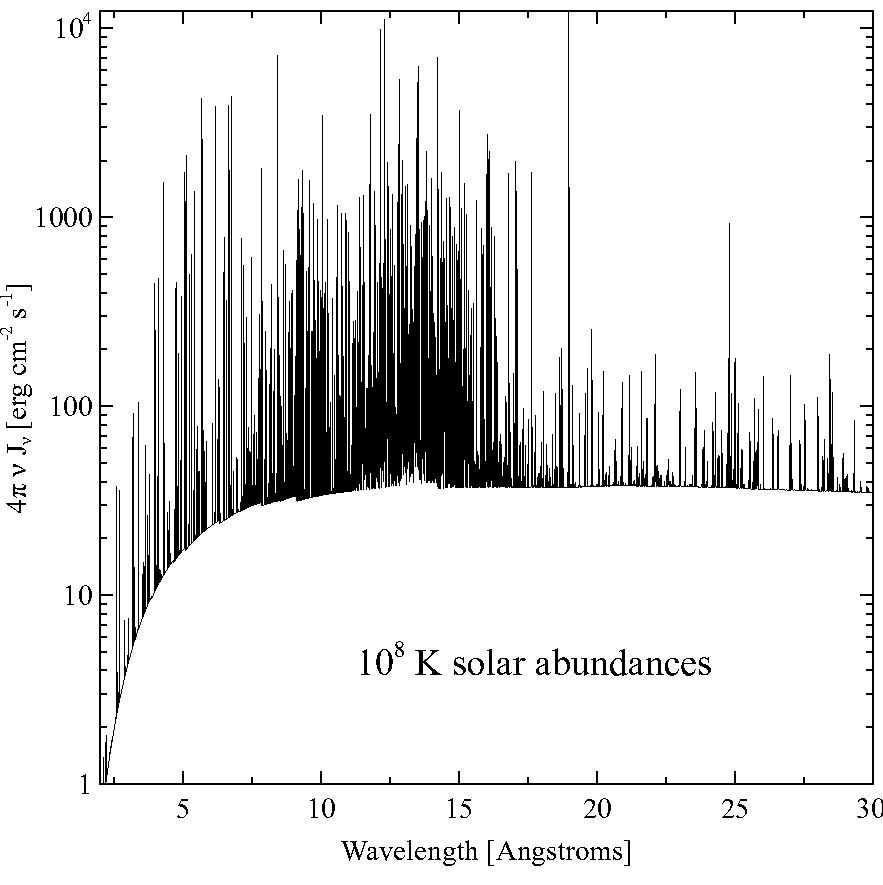
\includegraphics[clip=on,width=0.8\columnwidth,keepaspectratio]{coll_t7}
\end{center}
\end{figure}

\vspace{15 mm }
\LARGE
\emph{Cloudy \& Associates} \\
\Large
\href{http://www.nublado.org}{www.nublado.org} \\
\normalsize
\today
\end{center}
\end{titlepage}

%%%%%%%%%%%%%%%%%%%%%%%%%%%%%%%%%%%%%%%%%%%%%%%
% page with one figure and boilerplate text
\clearpage
{\small
\noindent
{\em Software:} Copyright \copyright\ 1978--2013 Gary J. Ferland and others. All rights reserved.

\vspace{1em}

\noindent
The software described in this documentation (\Cloudy) is subject
to a FreeBSD-style software license
contained in the file \cdFilename{license.txt} in the
root directory of the distributed files.
The list of co-authors is given in the file
\cdFilename{others.txt} in the same directory.
Use of this program is not restricted provided each use is
acknowledged upon publication.
The bibliographic reference to this version of \Cloudy\ is
``version xx.xx
of the code last described \citet{CloudyReview}.''
The version number, shown here as ``xx.xx'', should be
given.
This version number, along with a complete citation,
can be found by executing the code with the 
\cdCommand{print citation} command included in the input script.

\vspace{1em}

\noindent
\Cloudy\ is an evolving code.
You should confirm that you have the most recent
version of the code by checking the web site
\href{http://www.nublado.org}{www.nublado.org}.
The code has a
\href{http://tech.groups.yahoo.com/group/cloudy_simulations}{discussion board} with emailing list.
This will have announcements of any updates to the code.\par

\vspace{1em}

\noindent
Portions of the documentation have been published, and are copyrighted by, the
American Astronomical Society, the Astronomical Society of the Pacific, and
the Royal Astronomical Society. The remainder of the documentation is subject
to the following FreeBSD format documentation license:

\vspace{1em}

\noindent
{\em Documentation:} Copyright \copyright\ 1978--2013 Gary J. Ferland and others. All rights reserved.

\vspace{1em}

\noindent
Redistribution and use of the documentation (all parts of \Hazy\ and the
Quick Start Guide) in source (\LaTeX) and `compiled' forms (PDF, PostScript,
HTML and so forth) with or without modification, are permitted provided that
the following conditions are met:

\begin{enumerate}
\item
Redistributions of source code (\LaTeX) must retain the above copyright notice,
this list of conditions and the following disclaimer as the first lines of
the file \cdFilename{license\_doc.txt} in the root directory unmodified.
\item
Redistributions in compiled form (converted to PDF, PostScript, XML, HTML and
other formats) must reproduce the above copyright notice, this list of
conditions and the following disclaimer in the documentation and/or other
materials provided with the distribution.
\end{enumerate}

\noindent
{\em This documentation is provided by the \Cloudy\ project ``as is'' and any express
or implied warranties, including, but not limited to, the implied warranties
of merchantability and fitness for a particular purpose are disclaimed. In no
event shall the  \Cloudy\  project be liable for any direct, indirect, incidental,
special, exemplary, or consequential damages (including, but not limited to,
procurement of substitute goods or services; loss of use, data, or profits; or
business interruption) however caused and on any theory of liability, whether
in contract, strict liability, or tort (including negligence or otherwise)
arising in any way out of the use of this documentation, even if advised of
the possibility of such damage.}\par
}

\vspace{5mm}
\noindent
{\small
{\em Cover image:} The spectrum emitted by a cloud with solar abundances,
a temperature of 10$^7$~K, a density of 10$^{10} \pcc$, and a column density
of 10$^{15} \pscm$.  This shows recent improvements in the X-ray spectrum
and was done with the test case \cdFilename{coll\_t7.in} located in
\cdFilename{tsuite/auto}.  The command
\cdCommand{set continuum resolution 0.1} was added to
increase the continuum resolution by a factor of ten.
}
\clearpage

%%%%%%%%%%%%%%%%%%%%%%%%%%%%%%%%%%%%%%%%%%%%%%%
% table of contents page - only include top two levels
\setcounter{tocdepth}{2}
\tableofcontents
\listoffigures
\listoftables

\clearpage
\mainmatter
\chapter{OUTPUT}
% !TEX root = hazy2.tex
\label{sec:output}

\section{Overview}

This section defines the output produced by \Cloudy.  Each section begins
with a sample of the output described, and then goes on to describe the
meaning of the printout in greater detail.  The output actually shown is
from the Orion \hii\ Region / PDR / molecular cloud test case
(\cdFilename{orion\_hii\_pdr\_pp.in)}.

\section{Header Information}

Several lines of output echo the input commands and outline some
properties of the initial continuum.

{\setverbatimfontsize{\tiny}
\begin{verbatim}
                                  Cloudy 06.01.02

**************************************06Jan02**************************************
*                                                                                 *
* title the Orion HII Region / PDR / Molecular cloud with an open geometry        *
* c                                                                               *
* c commands controlling continuum =========                                      *
* c the incident continuum is two parts                                           *
* c kurucz continuum and flux of photons striking cloud                           *
* c this is the photosphere of the OVI star, its temperature and phi(H)           *
* table star kurucz 39600K                                                        *
* phi(H) 13                                                                       *
* c this adds the observed hot brems                                              *
* c its temperature (as log of T) and the flux of                                 *
* c photons striking the cloud                                                    *
* brems 6                                                                         *
* phi(h) 10                                                                       *
* c                                                                               *
* c cosmic rays are important for pdr chemistry                                   *
* cosmic rays, background                                                         *
* c                                                                               *
* c commands controlling geometry  =========                                      *
* c this turns off the stop temperature option                                    *
* c so the sim will not stop due to temperature                                   *
* stop temperature off                                                            *
* c this sets the thickness of the HII region & PDR                               *
* stop thickness 0.5 linear parsec                                                *
* c this will result in a milli gauss B-field in molecular region                 *
* magnetic field -5 gauss                                                         *
* c assume constant pressure                                                      *
* constant pressure                                                               *
* set nend 2000                                                                   *
* c                                                                               *
* c other commands for details     =========                                      *
* failures 3                                                                      *
* c mimic existence of unmodeled molecular gas                                    *
* double                                                                          *
* c iterate since lines optically thick                                           *
* iterate                                                                         *
* c set microturbulence in equipartition with B field                             *
* turbulence equipartition                                                        *
* c set the line width so lines appear on the save continuum                     *
* set SaveLwidth 10 km/s                                                         *
* c                                                                               *
* c commands for density & abundances =========                                   *
* c this is the log of the initial H density, cm-3                                *
* hden 4                                                                          *
* c this will speed up the calculation a bit                                      *
* init file="ism.ini"                                                             *
* c this uses HII region abundances, but no grains                                *
* abundances hii region no grains                                                 *
* c this uses orion grains                                                        *
* grains orion                                                                    *
* >>>> mie_read_opc reading file -- graphite_orion_10.opc                    <<<< *
* >>>> mie_read_opc reading file -- silicate_orion_10.opc                    <<<< *
* c turn on PAHs, with an abundance that depends on H0 fraction,                  *
* c as suggested by long-slit observations of Orion bar,                          *
* c with an abundance 3x larger than default built into the code                  *
* grains pah function 3                                                           *
* >>>> mie_read_opc reading file -- pah1_bt94_10.opc                         <<<< *
* c                                                                               *
* c commands controlling output    =========                                      *
* c print lots of faint CO lines                                                  *
* print line faint -4                                                             *
* c normalize to Ha                                                               *
* normalize to "H  1" 6563                                                        *
* c                                                                               *
* c orion hii pdr pp.in                                                           *
* c class hii pdr                                                                 *
*                                                                                 *
***********************************************************************************
\end{verbatim}
}

This begins with the version number of \Cloudy, the date that the version
was released, in the form yy.mm.dd.
The following line gives this date
in another form.

All of the input command lines, with the exception of those starting
with a \#, \%, or *, are echoed before the calculation begins,
and are saved
to be reprinted after the calculation is completed.
{\setverbatimfontsize{\tiny}
\begin{verbatim}
           3198CellPeak1.00E+00   Lo 9.99e-09=912.21cm   Hi-Con:1.20E+02 Ryd   E(hi):7.35E+06Ryd     E(hi):     100.01 MeV
           I(nu>1ryd):   2.4792   Average nu:1.382E+00   I( X-ray):  -1.6194   I(BalC):   2.8255     Phi(BalmrC):  13.7081
           phi(1.0-1.8):12.9508   phi(1.8-4.0): 12.033   phi(4.0-20):  9.388   phi(20--):  7.634     Ion pht flx:1.001E+13
           I(gam ray):   0.0000   phi(gam r):   0.0000   I(Infred):   1.5064   Alf(ox):   0.0000     Total inten:   3.0012
           U(1.0----):3.339E-02   U(4.0----):8.293E-06   T(En-Den):4.586E+01   T(Comp):3.532E+04     nuJnu(912A):5.422E+02
           Occ(FarIR):2.911E+08   Occ(H n=6):1.326E-11   Occ(1Ryd):2.470E-14   Occ(4R):5.400E-20     Occ (Nu-hi):1.201E-32
           Tbr(FarIR):4.835E+05   Tbr(H n=6):5.816E-08   Tbr(1Ryd):3.905E-09   Tbr(4R):3.413E-14     Tbr (Nu-hi):2.269E-25
\end{verbatim}
}
This block of information describes the continuum that strikes the
illuminated face of the cloud.
The full block of information is shown above,
and in the following discussion each line is given again
just before it is described.
{\setverbatimfontsize{\tiny}
\begin{verbatim}
           3198CellPeak1.00E+00   Lo 9.99e-09=912.21cm   Hi-Con:1.20E+02 Ryd   E(hi):7.35E+06Ryd     E(hi):     100.01 MeV
\end{verbatim}
}

This gives the number of numerical frequency cells in the continuum
followed by the energy (in Ryd) of the peak of hydrogen-ionizing
continuum.
This is the point with the largest flux density per unit energy interval
($J_\nu$).
Next is the energy of the low-energy limit of the continuum, in both
Ryd and cm.
The last two numbers are the energies of the high-energy limit
of the continuum in Ryd and MeV.
{\setverbatimfontsize{\tiny}
\begin{verbatim}
                 I(nu>1ryd):   2.4792   Average nu:1.382E+00   I( X-ray):  -1.6194   I(BalC):   2.8255     Phi(BalmrC):  13.7081
\end{verbatim}
}

This line gives the intensity or luminosity of the continuum source.
Luminosities are printed if the inner radius of the cloud is specified.
The units will be energy radiated by the central object into
$4\pi$~sr [erg s$^{-1}$].
If an inner radius is not set then the code will compute the intensity
case and give the emission per unit area of cloud surface.
This is loosely
called the intensity but is more formally $4\pi J$ where $J$ is the proper mean
intensity [erg cm$^{-2}$ s$^{-1}$ sr$^{-1}$ for an emission line; AGN3
Appendix~1].

The line gives the log of the energy (erg s$^{-1}$ cm$^{-2}$
or erg s$^{-1}$, depending
on whether it is the intensity or luminosity case) in the hydrogen-ionizing
continuum (1 Ryd $\le h\nu < 100$~MeV), and the average energy of the
hydrogen-ionizing continuum, in Ryd, weighted by photon number;
\begin{equation}
\left\langle {h\nu } \right\rangle  = \frac{{\int_{1\,Ryd}^\infty  {4\,\pi
\;{J_\nu }\;d{\kern 1pt} \nu } }}{{\int_{1\;Ryd}^\infty  {4\,\pi \;{J_\nu
}/h\nu \;d{\kern 1pt} \nu } }}\quad [\mathrm{Ryd}] .% (400)
\end{equation}
The log of the energy in the X-ray continuum (20.6 Ryd $\le h\nu\le  7676$~Ryd) is
followed by the log of the energy (erg s$^{-1}$ cm$^{-2}$ or erg s$^{-1}$) and the number
of photons (cm$^{-2}$ s$^{-1}$ or s$^{-1}$) in the Balmer continuum (0.25 Ryd to 1.0 Ryd).
{\setverbatimfontsize{\tiny}
\begin{verbatim}
                 phi(1.0-1.8):12.9508   phi(1.8-4.0): 12.033   phi(4.0-20):  9.388   phi(20--):  7.634     Ion pht flx:1.001E+13
\end{verbatim}
}

The third line gives the log of the number of photons
(cm$^{-2}$~s$^{-1}$ or s$^{-1}$)
in four frequency bins (1.0 Ryd $\le h\nu < 1.807$ Ryd, 1.807 Ryd
$\le h\nu < 4.0$ Ryd, 4.0 Ryd $\le h\nu < 20.6$ Ryd,
and 20.6 Ryd $\le h\nu < 7676$ Ryd).
The last number ``Ion pht flx'' is the flux of hydrogen ionizing photons;
\begin{equation}
\Phi \left( {{{\mathrm{H}}^{\mathrm{0}}}} \right) = \frac{{Q\left(
{{{\mathrm{H}}^{\mathrm{0}}}} \right)}}{{4\pi \,{r^2}}}\quad
  [\mathrm{cm}^{-2} \mathrm{s}^{-1}].% (401)
\end{equation}
In this equation $Q(\mathrm{H}^0$) is the total number of
hydrogen-ionizing photons
emitted by the central object (s$^{-1}$), and $r$ is the
separation between the
center of the central object and the illuminated face of the cloud.  Unlike
the majority of the quantities printed in the header,
$\Phi(\mathrm{H}^0$) (per unit area)
is always printed, never $Q(\mathrm{H}^0$) (into 4$\pi$~sr).
{\setverbatimfontsize{\tiny}
\begin{verbatim}
                 I(gam ray):   0.0000   phi(gam r):   0.0000   I(Infred):   1.5064   Alf(ox):   0.0000     Total inten:   3.0012
\end{verbatim}
}

The fourth line of the header gives some information about the low and
high energy portions of the incident continuum.
The first number is the
log of the luminosity or intensity in the gamma-ray ($\sim $100 keV  to
$\sim$100 MeV)
continuum.
The second number is the log of the number of photons over this
energy range.
The third number is the log of the luminosity in the continuum
between 0.25 Ryd and the lowest energy considered,
presently an energy of \emm .
All of these entries are either per unit area, or radiated
into $4\pi$~sr, depending on whether the intensity or luminosity case was
specified.

The entry ``Alf(ox)'' is the spectral index $\alpha_{ox}$,
defined as in Zamorani
et al. (1981), except for the difference in sign convention.
This is the
spectral index which would describe the continuum between 2 keV (147 Ryd)
and 2500\AA\ (0.3645 Ryd) if the continuum could be described
as a single power-law, that is,
\begin{equation}
\frac{{{f_\nu }\left( {2\;{\mathrm{keV}}} \right)}}{{{f_\nu }\left(
{2500\;{\mathrm{{\AA}}}} \right)}} = {\left( {\frac{{{\nu
_{2\;{\mathrm{keV}}}}}}{{{\nu _{2500\;{\mathrm{{\AA}}}}}}}} \right)^\alpha } =
{403.3^\alpha }.% (402)
\end{equation}
The definition of $\alpha_{ox}$ used here is slightly different from that of Zamorani
et al. since implicit negative signs are \emph{never} used by \Cloudy.  Typical
AGN have $\alpha_{ox} \sim  -1.4$.
If no X-rays are present then
$\alpha_{ox} = 0$.
The last number
on the line is the log of the total energy in the continuum between
\emm\ and \egamrymev .
{\setverbatimfontsize{\tiny}
\begin{verbatim}
           log L/Lsun:   3.9743   Abs bol mg:  -5.1858   Abs V mag:   2.4170   Bol cor:  -7.6028     nuFnu(Bbet):  34.5867
\end{verbatim}
}

This line is optional, depending on whether the luminosity or intensity
case is specified.  (It was not printed in this model since we are working
in the intensity case but a sample is shown).  This is printed in the
luminosity case.  First comes the log of the total luminosity in the
continuum in solar units.  The absolute bolometric magnitude, absolute V
magnitude, and the bolometric correction, are then given, followed by the
log of the continuum specific luminosity $[\nu F_\nu(\mathrm{H}\beta)]$
at the wavelength of H$\beta [\mathrm{erg\,s}^{-1}]$.
{\setverbatimfontsize{\tiny}
\begin{verbatim}
                 U(1.0----):3.339E-02   U(4.0----):8.293E-06   T(En-Den):4.586E+01   T(Comp):3.532E+04     nuJnu(912A):5.422E+02
\end{verbatim}
}
This line begins with two ionization parameters.
The first is the
dimensionless ratio of ionizing photon to hydrogen densities,
defined as
\begin{equation}
U \equiv \frac{{\Phi \left( {{{\mathrm{H}}^{\mathrm{0}}}}
\right)}}{{{n_{\mathrm{H}}}c}},%  (403)
\end{equation}
where $n_H$ is the total hydrogen density.
The second number is defined in
a similar way, but the numerator is the number of photons with energies
greater than 4 Ryd (i.e., helium-ionizing).
The third number is the
equivalent black-body temperature corresponding to the energy density $u$
at the illuminated face of the cloud, from the incident continuum and
Stefan's radiation density constant $a$;
\begin{equation}
{T_u} \equiv {\left( {L/4\pi \,{r^2}ac} \right)^{1/4}}\quad
 [\mathrm{K}] .% (404)
\end{equation}
T(Comp) is the Compton temperature of the incident radiation
field.\footnote{For a blackbody radiation field $T_{Compton}$ is roughly 4\% lower than
the blackbody color temperature $T_{color}$ when the energy density temperature
$T_u$ is $> T_{color}$.
Only when $T_u \equiv T_{color}$ does induced Compton heating cause
$T_{Compton} \equiv T_{color}$.
If $T_u > T_{color}$  then $T_{Compton} >
T_{color}$ because of induced
Compton heating.
All of the relevant physics is included in the Compton
temperature printed here.}  The
last number is $4\pi \nu J_\nu(912 \AA )$, the flux at 912\AA\ (erg
cm$^{-2}$ s$^{-1}$), where
$J_\nu$ is the mean intensity of the incident continuum (\citealp{Mihalas1978}).
{\setverbatimfontsize{\tiny}
\begin{verbatim}
           Occ(FarIR):2.911E+08   Occ(H n=6):1.326E-11   Occ(1Ryd):2.470E-14   Occ(4R):5.400E-20     Occ (Nu-hi):1.201E-32
           Tbr(FarIR):4.835E+05   Tbr(H n=6):5.816E-08   Tbr(1Ryd):3.905E-09   Tbr(4R):3.413E-14     Tbr (Nu-hi):2.269E-25
\end{verbatim}
}

These lines give dimensionless photon occupation numbers $\eta(\nu)$,
for the incident continuum at several energies.
The occupation number is defined as
\begin{equation}
{\eta _\nu } \equiv {J_\nu }\left( \nu  \right)\,{\left( {\frac{{2h{\nu
^3}}}{{{c^2}}}} \right)^{ - 1}},% (405)
\end{equation}
and the incident continuum brightness temperature ${T_b}( \nu  )$, [K] is defined as
\begin{equation}
{T_b}\left( \nu  \right) \equiv {J_\nu }\left( \nu  \right){\left(
{\frac{{2k{\kern 1pt} {\nu ^2}}}{{{c^2}}}} \right)^{ - 1}}\quad  [\mathrm{K}].% (406)
\end{equation}
These energies correspond to the lowest frequency considered
(presently \emm );
the ionization potential of the $n = 6$ level of hydrogen
(1/36 Ryd); one Rydberg; four Rydbergs, and the high-energy limit of the
incident continuum.
The energy where the last number is evaluated depends
on the continuum shape.
The energy is given by the fifth number on the
first line of the continuum output.

\section{Chemical composition}
{\setverbatimfontsize{\tiny}
\begin{verbatim}
                                                  Gas Phase Chemical Composition
        H :  0.0000  He: -1.0223  C : -3.5229  N : -4.1549  O : -3.3979  Ne: -4.2218  Mg: -5.5229  Si: -5.3979  S : -5.0000
                                               Cl: -7.0000  Ar: -5.5229  Fe: -5.5229

                                                    Grain Chemical Composition
                                  C : -3.6259  O : -3.9526  Mg: -4.5547  Si: -4.5547  Fe: -4.5547

                                                  Number of grains per hydrogen
                                            Carbonaceous: -14.166  silicate: -14.103
\end{verbatim}
}

The chemical composition of the cloud comes next.
The three blocks of
numbers give the gas-phase abundances of the elements, the abundances
contained in grains, and the number of each type of grains per unit hydrogen.
The numbers are the logs of the number densities of the elements, relative
to the gas-phase hydrogen abundance of unity (so, 0 on the log scale).
Only the active elements are included (those turned off with the \cdCommand{elements off} command are not printed).
If grains are not present then the second
two blocks are not printed.

\section{Comments before or during the calculation}

The code may print comments as the calculation proceeds.
These are
printed with the start of the comment in capital letters to make them easy
to find with a script.
The comments fall into three categories:
\begin{description}
\item[DISASTER] something has unexpectedly caused the calculation to stop.
The results are bogus and should not be trusted.
The code should immediately
return to the calling program.

\item[PROBLEM] something did not go as expected but the calculation is
continuing.  This might be a convergence failure at a point in the cloud.
This is an indication that the code was having difficulties and a few of
these can occur in a normal set of calculations.
The predictions can be
used if only a few occur and if the comments at the end of the calculation
(see page \pageref{sec:CommentsAfterCalculation} below)
do not identify other problems.

\item[NOTE] this gives advice about the calculation.  These can be ignored
if you prefer.
\end{description}

\section{Zone Results}

Next comes a summary of the conditions in the first and last zone.
This print out is done in routine \cdRoutine{PrtZone} which should
be consulted if there are any questions.
The following is the output produced for one zone.
Details follow.
{\setverbatimfontsize{\tiny}
\begin{verbatim}
####  1  Te:9.361E+03 Hden:1.000E+04 Ne:1.101E+04 R:1.000E+30 R-R0:5.223E+11 dR:1.045E+12 NTR:  3 Htot:3.461E-16 T912: 1.48e-05###
 Hydrogen      1.47e-04 1.00e+00 H+o/Hden 1.00e+00 4.12e-12 H-    H2 8.43e-17 4.10e-13 H2+ HeH+ 1.13e-12 Ho+ ColD 1.54e+12 1.04e+16
 Helium        6.57e-04 9.45e-01 5.47e-02 He I2SP3 3.52e-06 Comp H,C 1.75e-22 4.64e-23 Fill Fac 1.00e+00 Gam1/tot 1.00e+00
 He singlet n  6.54e-04 2.35e-11 6.59e-18 2.09e-18 3.18e-18 2.52e-18 He tripl 3.52e-06 9.32e-16 7.41e-18 4.77e-17 7.56e-18
 Pressure      NgasTgas 2.06e+08 P(total) 2.84e-08 P( gas ) 2.84e-08 P(Radtn) 1.79e-11 Rad accl 3.51e-05 ForceMul 3.33e+03
               Texc(La) 4.21e+03 T(contn) 4.59e+01 T(diffs) 2.03e+00 nT (c+d) 1.16e+07 Prad/Gas 6.30e-04 Pmag/Gas 2.80e-04
 gra-orion01*  DustTemp 2.12e+02 Pot Volt 5.32e+00 Chrg (e) 1.21e+02 drf cm/s 4.83e+03 Heating: 4.26e-18 Frac tot 1.23e-02
 gra-orion02*  DustTemp 2.02e+02 Pot Volt 5.08e+00 Chrg (e) 1.43e+02 drf cm/s 5.26e+03 Heating: 3.69e-18 Frac tot 1.07e-02
 gra-orion03*  DustTemp 1.91e+02 Pot Volt 4.86e+00 Chrg (e) 1.70e+02 drf cm/s 5.60e+03 Heating: 3.21e-18 Frac tot 9.26e-03
 gra-orion04*  DustTemp 1.81e+02 Pot Volt 4.66e+00 Chrg (e) 2.01e+02 drf cm/s 5.86e+03 Heating: 2.79e-18 Frac tot 8.06e-03
 gra-orion05   DustTemp 1.70e+02 Pot Volt 4.47e+00 Chrg (e) 2.39e+02 drf cm/s 6.07e+03 Heating: 2.43e-18 Frac tot 7.03e-03
 gra-orion06   DustTemp 1.60e+02 Pot Volt 4.30e+00 Chrg (e) 2.85e+02 drf cm/s 6.22e+03 Heating: 2.13e-18 Frac tot 6.16e-03
 gra-orion07   DustTemp 1.50e+02 Pot Volt 4.15e+00 Chrg (e) 3.40e+02 drf cm/s 6.33e+03 Heating: 1.87e-18 Frac tot 5.41e-03
 gra-orion08   DustTemp 1.40e+02 Pot Volt 4.02e+00 Chrg (e) 4.07e+02 drf cm/s 6.42e+03 Heating: 1.65e-18 Frac tot 4.77e-03
 gra-orion09   DustTemp 1.31e+02 Pot Volt 3.91e+00 Chrg (e) 4.89e+02 drf cm/s 6.48e+03 Heating: 1.46e-18 Frac tot 4.21e-03
 gra-orion10   DustTemp 1.22e+02 Pot Volt 3.80e+00 Chrg (e) 5.89e+02 drf cm/s 6.54e+03 Heating: 1.29e-18 Frac tot 3.73e-03
 sil-orion01*  DustTemp 1.55e+02 Pot Volt 2.85e+00 Chrg (e) 6.44e+01 drf cm/s 1.45e+04 Heating: 2.44e-18 Frac tot 7.06e-03
 sil-orion02*  DustTemp 1.49e+02 Pot Volt 2.70e+00 Chrg (e) 7.58e+01 drf cm/s 1.62e+04 Heating: 2.09e-18 Frac tot 6.03e-03
 sil-orion03*  DustTemp 1.43e+02 Pot Volt 2.57e+00 Chrg (e) 8.92e+01 drf cm/s 1.77e+04 Heating: 1.78e-18 Frac tot 5.15e-03
 sil-orion04   DustTemp 1.37e+02 Pot Volt 2.44e+00 Chrg (e) 1.05e+02 drf cm/s 1.91e+04 Heating: 1.53e-18 Frac tot 4.42e-03
 sil-orion05   DustTemp 1.31e+02 Pot Volt 2.33e+00 Chrg (e) 1.24e+02 drf cm/s 2.02e+04 Heating: 1.32e-18 Frac tot 3.81e-03
 sil-orion06   DustTemp 1.26e+02 Pot Volt 2.24e+00 Chrg (e) 1.47e+02 drf cm/s 2.11e+04 Heating: 1.14e-18 Frac tot 3.30e-03
 sil-orion07   DustTemp 1.20e+02 Pot Volt 2.15e+00 Chrg (e) 1.76e+02 drf cm/s 2.18e+04 Heating: 9.93e-19 Frac tot 2.87e-03
 sil-orion08   DustTemp 1.15e+02 Pot Volt 2.08e+00 Chrg (e) 2.10e+02 drf cm/s 2.23e+04 Heating: 8.67e-19 Frac tot 2.50e-03
 sil-orion09   DustTemp 1.10e+02 Pot Volt 2.01e+00 Chrg (e) 2.52e+02 drf cm/s 2.26e+04 Heating: 7.60e-19 Frac tot 2.20e-03
 sil-orion10   DustTemp 1.06e+02 Pot Volt 1.96e+00 Chrg (e) 3.03e+02 drf cm/s 2.28e+04 Heating: 6.69e-19 Frac tot 1.93e-03
 pah-bt9401 *  DustTemp 3.41e+02 Pot Volt 6.60e+00 Chrg (e) 1.06e+00 drf cm/s 1.97e+02 Heating: 9.29e-22 Frac tot 2.68e-06
 pah-bt9402 *  DustTemp 3.44e+02 Pot Volt 6.64e+00 Chrg (e) 1.28e+00 drf cm/s 2.13e+02 Heating: 1.01e-21 Frac tot 2.92e-06
 pah-bt9403 *  DustTemp 3.47e+02 Pot Volt 6.61e+00 Chrg (e) 1.49e+00 drf cm/s 2.37e+02 Heating: 1.07e-21 Frac tot 3.08e-06
 pah-bt9404 *  DustTemp 3.50e+02 Pot Volt 6.54e+00 Chrg (e) 1.70e+00 drf cm/s 2.67e+02 Heating: 1.09e-21 Frac tot 3.16e-06
 pah-bt9405 *  DustTemp 3.53e+02 Pot Volt 6.44e+00 Chrg (e) 1.92e+00 drf cm/s 3.02e+02 Heating: 1.09e-21 Frac tot 3.16e-06
 pah-bt9406 *  DustTemp 3.55e+02 Pot Volt 6.45e+00 Chrg (e) 2.22e+00 drf cm/s 3.29e+02 Heating: 1.13e-21 Frac tot 3.26e-06
 pah-bt9407 *  DustTemp 3.57e+02 Pot Volt 6.47e+00 Chrg (e) 2.54e+00 drf cm/s 3.60e+02 Heating: 1.17e-21 Frac tot 3.38e-06
 pah-bt9408 *  DustTemp 3.59e+02 Pot Volt 6.43e+00 Chrg (e) 2.87e+00 drf cm/s 4.00e+02 Heating: 1.18e-21 Frac tot 3.40e-06
 pah-bt9409 *  DustTemp 3.61e+02 Pot Volt 6.46e+00 Chrg (e) 3.27e+00 drf cm/s 4.35e+02 Heating: 1.20e-21 Frac tot 3.46e-06
 pah-bt9410 *  DustTemp 3.63e+02 Pot Volt 6.48e+00 Chrg (e) 3.71e+00 drf cm/s 4.74e+02 Heating: 1.22e-21 Frac tot 3.52e-06
 Carbon        6.76e-07 1.91e-02 9.70e-01 1.10e-02 1.77e-04 2.36e-09 0.00e+00 H2O+/O   0.00e+00 OH+/Otot 0.00e+00 Hex(tot) 0.00e+00
 Nitrogen      1.60e-06 1.72e-02 9.69e-01 1.41e-02 4.77e-05 1.34e-07 9.81e-14 0.00e+00 O2/Ototl 0.00e+00 O2+/Otot 0.00e+00
 Oxygen        9.23e-06 1.17e-01 8.59e-01 2.47e-02 6.97e-05 9.60e-08 4.83e-11 0.00e+00 0.00e+00
 Neon          5.77e-05 3.93e-01 5.95e-01 1.17e-02 7.25e-05 5.08e-08 1.99e-12 1.47e-16 0.00e+00 0.00e+00 0.00e+00
 Magnesium     6.41e-06 7.31e-03 9.65e-01 2.74e-02 1.76e-04 5.41e-07 2.86e-10 3.72e-14 9.96e-19 0.00e+00 0.00e+00 0.00e+00 0.00e+00
 Silicon    0  1.13e-07 8.39e-03 8.16e-01 1.56e-01 1.86e-02 4.68e-05 3.08e-08 5.13e-12 1.63e-16 0.00e+00 0.00e+00 0.00e+00 0.00e+00
 Sulphur    0  7.25e-08 7.46e-03 9.03e-01 8.81e-02 1.60e-03 1.67e-04 5.91e-06 9.11e-10 3.49e-14 3.20e-19 0.00e+00 0.00e+00 0.00e+00
 Chlorine   0  2.51e-07 1.32e-02 9.57e-01 2.92e-02 7.57e-04 5.50e-05 7.07e-07 9.54e-09 2.94e-13 2.17e-18 0.00e+00 0.00e+00 0.00e+00
 Argon      0  9.50e-08 2.83e-03 9.69e-01 2.73e-02 4.35e-04 2.65e-05 3.24e-07 1.53e-09 1.16e-11 8.21e-17 0.00e+00 0.00e+00 0.00e+00
 Iron       0  1.78e-08 2.88e-04 1.08e-01 8.56e-01 3.26e-02 2.33e-03 2.33e-05 2.30e-07 1.28e-10 1.94e-14 9.07e-19 0.00e+00 0.00e+00
\end{verbatim}
}

The results of calculations for the first and last zones are always
printed.
Results for intermediate zones can be printed if desired (see
the \cdCommand{print every} command).
The following is a line-by-line description of
the output produced for each printed zone.
{\setverbatimfontsize{\tiny}
\begin{verbatim}
####  1  Te:9.361E+03 Hden:1.000E+04 Ne:1.101E+04 R:1.000E+30 R-R0:5.223E+11 dR:1.045E+12 NTR:  3 Htot:3.461E-16 T912: 1.48e-05###
\end{verbatim}
}

The line begins with a series of \#\#\#\# characters to make it easy
to locate with an editor.
The zone number is the first number and it is
followed by the electron temperature of the zone (``Te'').
A lower case
``u'' will appear before the ``Te'' if the temperature solution is possibly
thermally unstable.
This occurs when the derivative of the net cooling
with respect to temperature is negative.
This is discussed further in the
section on thermal stability problems starting on page
\pageref{sec:ThermalStabilityProblems} below.
The total hydrogen (``Hden'')
and electron (``Ne'') densities (cm$^{-3}$) follow.
The next number (``R'')
is the distance from the center of the central object to the center of the
zone.
The depth, the distance between the illuminated face of the cloud
and the center of the zone, (``R-R0'', or ``r-r$^{\mathrm{o}}$''),
and the thickness of
the zone (``dR'', or $\delta r$), (all are in cm), follow.
The inner edge of the
zone is $( {r - {r_o}} ) - \delta r/2$
from the illuminated face of the cloud.
The line ends with a number
indicating how many ionization iterations were needed for this zone to
converge (NTR), followed by the total heating\footnote{\Cloudy\ defines heating as the energy input by the freed photoelectron,
or $h\nu - $IP, where IP is the ionization potential of the atom or ion, and
$h\nu$ is the energy of the photon.  See AGN3 for more details.} (``Htot''; photoelectric
and otherwise, erg cm$^{-3}$ s$^{-1}$),
and the optical depth between the
\emph{illuminated}
face of the cloud and the \emph{outer} edge of the zone at the Lyman limit (T912;
the number is the \emph{total absorption} optical depth at 912\AA,
and not the
hydrogen Lyman-limit optical depth).
{\setverbatimfontsize{\tiny}
\begin{verbatim}
WIND; V:-7.000e+00km/s G:-0.00e+00 Accel: 8.62e-06 Fr(cont): 1.000 Fr(line): 0.000 Fr(dP): 0.000
\end{verbatim}
}

A line describing the velocity and acceleration of the zone is printed
if the cloud is a wind.
The numbers are the wind velocity at the outer
edge of the current zone (km s$^{-1}$), inward gravitational acceleration (cm s$^{-2}$), total outward radiative acceleration (cm s$^{-2}$),
and the fraction of
this acceleration caused by the incident continuum, line driving, and the
gradient of the radiation pressure.
{\setverbatimfontsize{\tiny}
\begin{verbatim}
P(Lines):(Mg 2  2796A 0.32) (Mg 2  2803A 0.20) (H  1  6563A 0.13) (H  1 1.875m 0.10) (Fe 2  1786A 0.06) (H  1  4861A 0.05)
\end{verbatim}
}
A line describing the source of the radiation pressure is generated if
the ratio of line radiation to gas pressure, $P_{rad}/P_{gas}$,
is greater than 5\%.
The line begins with the label ``P(Lines)'' and
continues with the fraction
of the total radiation pressure produced by that emission line, the
spectroscopic designation of the line, and its wavelength.
Up to twenty
lines can be printed, although in most cases only \la\
and a few others will dominate.
{\setverbatimfontsize{\tiny}
\begin{verbatim}
Hydrogen      1.47e-04 1.00e+00 H+o/Hden 1.00e+00 4.12e-12 H-    H2 8.43e-17 4.10e-13 H2+ HeH+ 1.13e-12 Ho+ ColD 1.54e+12 1.04e+16
\end{verbatim}
}

The line begins with the ratios $n(\mathrm{H}^0)/n(H_{tot})$ and
$n(\mathrm{H}^+)/n(\mathrm{H}_{tot})$ where
$H_{tot}$ is the total density in H all forms (including molecular).
If \cdCommand{print h-like departure coefficients} has been specified
then departure coefficients
are also printed on the following line.
Neutral hydrogen H$^0$ is defined
to be the total population of atomic hydrogen in all explicitly computed
bound levels.
Next comes ``H+o/Hden'', the ratio
$[n(\mathrm{H}^0) + n(\mathrm{H}^+)]/n(\mathrm{H}_{tot})$.

The following five numbers give densities of the negative hydrogen ion
and several molecules (\hminus, \htwo, H$_2^+$, and HeH$^+$)
relative to the total hydrogen density.
Note that, with this definition of the hydrogen density, a fully
molecular gas will have $n(\mathrm{H}2)/n(\mathrm{H})=0.5$.
These molecular abundances are
also expressed as departure coefficients if the
\cdCommand{print departure coefficients}
command occurs.
The last number is the H$^0$ and H$^+$ column densities
(cm$^{-2}$).
{\setverbatimfontsize{\tiny}
\begin{verbatim}
 H  1 1S-12    1.39e-01 3.43e-04 1.02e-03 1.02e-03 1.24e-03 1.62e-03 2.12e-03 2.73e-03 3.43e-03 4.23e-03 5.12e-03 6.12e-03 7.20e-03
 H  1  rest    8.39e-03 9.66e-03 1.10e-02 1.25e-02 1.41e-02 1.57e-02 1.75e-02 1.93e-02 2.13e-02 2.33e-02 2.54e-02 2.77e-02 3.00e-02
               3.24e-02 3.49e-02 3.75e-02 4.02e-02 4.30e-02 4.59e-02 4.89e-02 5.20e-02 5.51e-02 5.84e-02 6.18e-02 6.52e-02 6.88e-02
               7.24e-02 7.62e-02 8.00e-02 8.39e-02 8.79e-02 9.21e-02 9.63e-02 1.01e-01 1.05e-01 1.09e-01 1.14e-01 1.19e-01
\end{verbatim}
}
This information is only printed if the
\cdCommand{print H-like populations} command occurs.
The numbers give the populations of the \hO\ levels relative to the
ionized hydrogen density.
All of these populations usually are relative
to the ionized hydrogen density, but can also be printed as LTE departure
coefficients if the \cdCommand{print departure coefficients} command
is given.
{\setverbatimfontsize{\tiny}
\begin{verbatim}
Helium        6.57e-04 9.45e-01 5.47e-02 He I2SP3 3.52e-06 Comp H,C 1.75e-22 4.64e-23 Fill Fac 1.00e+00 Gam1/tot 1.00e+00
\end{verbatim}
}

The first three numbers are the total populations of the three ionization
stages of helium relative to the total helium abundance.
The population
of atomic helium is the sum of the total population in the triplets and
singlets, including the population of all explicitly computed levels of
each.
These populations can also be expressed as departure coefficients
if this option is set with the \cdCommand{print departure coefficients} command.
The
population of He~2$^3$~S, relative to the total helium abundance, follows.
The Compton heating and cooling rates (both erg cm$^{-3}$~s$^{-1}$) are next, followed
by the gas filling factor.
The last number is the fraction of the total
hydrogen ionizations that are caused by photoionization from the ground
state.
{\setverbatimfontsize{\tiny}
\begin{verbatim}
He singlet n  6.54e-04 2.35e-11 6.59e-18 2.09e-18 3.18e-18 2.52e-18 He tripl 3.52e-06 9.32e-16 7.41e-18 4.77e-17 7.56e-18
\end{verbatim}
}

The first numbers are the level populations of the $l$-levels within
$n=1$ to 3 of the He$^0$ singlets.
The next group consists of He$^0$ triplet populations
of $2S$, the three $2^3P_j$, levels and the $3S$, $3P$, and $3D$ levels.  All populations
are relative to the total helium abundance.
Departure coefficients are
also printed if requested.
{\setverbatimfontsize{\tiny}
\begin{verbatim}
Pressure      NgasTgas 2.06e+08 P(total) 2.84e-08 P( gas ) 2.84e-08 P(Radtn) 1.79e-11 Rad accl 3.51e-05 ForceMul 3.33e+03
              Texc(La) 4.21e+03 T(contn) 4.59e+01 T(diffs) 2.03e+00 nT (c+d) 1.16e+07 Prad/Gas 6.30e-04 Pmag/Gas 2.80e-04
\end{verbatim}
}

Some information concerning the pressure is printed.
The gas equation
of state includes thermal gas pressure, the radiation pressure due to trapped
line emission, magnetic and turbulent pressure, and the radiation pressure
due to absorption of the incident continuum.
The first number is the gas
pressure $n_{gas}\, T_{gas}$ (with units cm$^{-3}$~K), followed by the total pressure
(dynes cm$^{-2}$), and is followed by the gas pressure
$(n_{gas}\, kT_{gas})$ in dynes cm$^{-2}$.
The radiation pressure follows.  The second to last number is the
radiative acceleration (cm s$^{-2}$) at the inner edge of this zone.
The
radiative acceleration is computed with all continuous scattering and
absorption opacities included.  The last number is a force multiplier,
defined as in \citet{Tarter1973}, and is the ratio of total opacity
to electron scattering opacity.

The second line gives more information.
The line starts with
``Texc(La)'', the excitation temperature $T_{exc}$ of \la,
defined as
\begin{equation}
\frac{{n\left( {2p} \right)/g\left( {2p} \right)}}{{n\left( {1s}
\right)/g\left( {1s} \right)}} = \exp \left[ { - h\nu /k{T_{exc}}\left(
{L\alpha } \right)} \right].% (407)
\end{equation}
This is followed by the temperature corresponding to the energy density
of the attenuated incident continuum (``T(contn)'')
and the diffuse continua (``T(diffs)'').
This includes all trapped lines and diffuse continuous
emission.
The entry ``nT (c+d)''is the energy density of the sum of these
two continua expressed as an equivalent pressure $nT$ [cm$^{-3}$~K].
The line
ends with the ratios of the radiation to gas pressure ``Prad/Gas'' and the
ratio of magnetic to gas pressure ``Pmag/Gas''.

{\setverbatimfontsize{\tiny}
\begin{verbatim}
 gra-orion01*  DustTemp 2.12e+02 Pot Volt 5.32e+00 Chrg (e) 1.21e+02 drf cm/s 4.83e+03 Heating: 4.26e-18 Frac tot 1.23e-02
 gra-orion02*  DustTemp 2.02e+02 Pot Volt 5.08e+00 Chrg (e) 1.43e+02 drf cm/s 5.26e+03 Heating: 3.69e-18 Frac tot 1.07e-02
 gra-orion03*  DustTemp 1.91e+02 Pot Volt 4.86e+00 Chrg (e) 1.70e+02 drf cm/s 5.60e+03 Heating: 3.21e-18 Frac tot 9.26e-03
 gra-orion04*  DustTemp 1.81e+02 Pot Volt 4.66e+00 Chrg (e) 2.01e+02 drf cm/s 5.86e+03 Heating: 2.79e-18 Frac tot 8.06e-03
 gra-orion05   DustTemp 1.70e+02 Pot Volt 4.47e+00 Chrg (e) 2.39e+02 drf cm/s 6.07e+03 Heating: 2.43e-18 Frac tot 7.03e-03
 gra-orion06   DustTemp 1.60e+02 Pot Volt 4.30e+00 Chrg (e) 2.85e+02 drf cm/s 6.22e+03 Heating: 2.13e-18 Frac tot 6.16e-03
 gra-orion07   DustTemp 1.50e+02 Pot Volt 4.15e+00 Chrg (e) 3.40e+02 drf cm/s 6.33e+03 Heating: 1.87e-18 Frac tot 5.41e-03
 gra-orion08   DustTemp 1.40e+02 Pot Volt 4.02e+00 Chrg (e) 4.07e+02 drf cm/s 6.42e+03 Heating: 1.65e-18 Frac tot 4.77e-03
 gra-orion09   DustTemp 1.31e+02 Pot Volt 3.91e+00 Chrg (e) 4.89e+02 drf cm/s 6.48e+03 Heating: 1.46e-18 Frac tot 4.21e-03
 gra-orion10   DustTemp 1.22e+02 Pot Volt 3.80e+00 Chrg (e) 5.89e+02 drf cm/s 6.54e+03 Heating: 1.29e-18 Frac tot 3.73e-03
 sil-orion01*  DustTemp 1.55e+02 Pot Volt 2.85e+00 Chrg (e) 6.44e+01 drf cm/s 1.45e+04 Heating: 2.44e-18 Frac tot 7.06e-03
 sil-orion02*  DustTemp 1.49e+02 Pot Volt 2.70e+00 Chrg (e) 7.58e+01 drf cm/s 1.62e+04 Heating: 2.09e-18 Frac tot 6.03e-03
 sil-orion03*  DustTemp 1.43e+02 Pot Volt 2.57e+00 Chrg (e) 8.92e+01 drf cm/s 1.77e+04 Heating: 1.78e-18 Frac tot 5.15e-03
 sil-orion04   DustTemp 1.37e+02 Pot Volt 2.44e+00 Chrg (e) 1.05e+02 drf cm/s 1.91e+04 Heating: 1.53e-18 Frac tot 4.42e-03
 sil-orion05   DustTemp 1.31e+02 Pot Volt 2.33e+00 Chrg (e) 1.24e+02 drf cm/s 2.02e+04 Heating: 1.32e-18 Frac tot 3.81e-03
 sil-orion06   DustTemp 1.26e+02 Pot Volt 2.24e+00 Chrg (e) 1.47e+02 drf cm/s 2.11e+04 Heating: 1.14e-18 Frac tot 3.30e-03
 sil-orion07   DustTemp 1.20e+02 Pot Volt 2.15e+00 Chrg (e) 1.76e+02 drf cm/s 2.18e+04 Heating: 9.93e-19 Frac tot 2.87e-03
 sil-orion08   DustTemp 1.15e+02 Pot Volt 2.08e+00 Chrg (e) 2.10e+02 drf cm/s 2.23e+04 Heating: 8.67e-19 Frac tot 2.50e-03
 sil-orion09   DustTemp 1.10e+02 Pot Volt 2.01e+00 Chrg (e) 2.52e+02 drf cm/s 2.26e+04 Heating: 7.60e-19 Frac tot 2.20e-03
 sil-orion10   DustTemp 1.06e+02 Pot Volt 1.96e+00 Chrg (e) 3.03e+02 drf cm/s 2.28e+04 Heating: 6.69e-19 Frac tot 1.93e-03
 pah-bt9401 *  DustTemp 3.41e+02 Pot Volt 6.60e+00 Chrg (e) 1.06e+00 drf cm/s 1.97e+02 Heating: 9.29e-22 Frac tot 2.68e-06
 pah-bt9402 *  DustTemp 3.44e+02 Pot Volt 6.64e+00 Chrg (e) 1.28e+00 drf cm/s 2.13e+02 Heating: 1.01e-21 Frac tot 2.92e-06
 pah-bt9403 *  DustTemp 3.47e+02 Pot Volt 6.61e+00 Chrg (e) 1.49e+00 drf cm/s 2.37e+02 Heating: 1.07e-21 Frac tot 3.08e-06
 pah-bt9404 *  DustTemp 3.50e+02 Pot Volt 6.54e+00 Chrg (e) 1.70e+00 drf cm/s 2.67e+02 Heating: 1.09e-21 Frac tot 3.16e-06
 pah-bt9405 *  DustTemp 3.53e+02 Pot Volt 6.44e+00 Chrg (e) 1.92e+00 drf cm/s 3.02e+02 Heating: 1.09e-21 Frac tot 3.16e-06
 pah-bt9406 *  DustTemp 3.55e+02 Pot Volt 6.45e+00 Chrg (e) 2.22e+00 drf cm/s 3.29e+02 Heating: 1.13e-21 Frac tot 3.26e-06
 pah-bt9407 *  DustTemp 3.57e+02 Pot Volt 6.47e+00 Chrg (e) 2.54e+00 drf cm/s 3.60e+02 Heating: 1.17e-21 Frac tot 3.38e-06
 pah-bt9408 *  DustTemp 3.59e+02 Pot Volt 6.43e+00 Chrg (e) 2.87e+00 drf cm/s 4.00e+02 Heating: 1.18e-21 Frac tot 3.40e-06
 pah-bt9409 *  DustTemp 3.61e+02 Pot Volt 6.46e+00 Chrg (e) 3.27e+00 drf cm/s 4.35e+02 Heating: 1.20e-21 Frac tot 3.46e-06
 pah-bt9410 *  DustTemp 3.63e+02 Pot Volt 6.48e+00 Chrg (e) 3.71e+00 drf cm/s 4.74e+02 Heating: 1.22e-21 Frac tot 3.52e-06
\end{verbatim}
}

Some properties of the grain populations are printed if they are present.
Each line gives the results of calculations for a specific type and size
of grain.
Graphite and silicate are normally included when grains are
present.
Each line begins with the name of the grain and an asterisk appears
if quantum heating was important for the species.
Quantum heating is only
computed if it is significant due to its computational expense.
The
remainder of the line gives the equilibrium temperature of the grain, the
potential in volts, the charge, the drift velocity, the gas heating (erg
cm$^{-3}$ s$^{-1}$) due to grain electron photoemission, and the dimensionless fraction
of the total gas heating due to grain electron photoemission.
For
quantum-heated grains the temperature is the average weighted by $T^4$.

{\setverbatimfontsize{\tiny}
\begin{verbatim}
Molecules     CH/Ctot: 3.65e-04 CH+/Ctot 5.82e-13 CO/Ctot: 5.52e-01 CO+/Ctot 1.95e-14 H2O/Otot 3.27e-09 OH/Ototl 4.18e-11
\end{verbatim}
}

A line giving relative abundances of some molecules is printed if the
molecular fraction is significant.
All molecular abundances are relative
to either the total carbon or total oxygen abundance (this is indicated
in the label for each).
In order, the molecules are CH, CH$^+$, CO,
CO$^+$, H$_2$O, and OH.
{\setverbatimfontsize{\tiny}
\begin{verbatim}
Lithium       8.94e-02 9.11e-01 9.53e-10 0.00e+00 Berylliu 9.99e-01 6.40e-04 6.38e-05 7.06e-10 0.00e+00 sec ion: 7.66e-15

Abundances of each stage of ionization of lithium and beryllium relative
to the total gas-phase abundance of the element are followed by the
suprathermal secondary ionization rate [s$^{-1}$].
{\setverbatimfontsize{\tiny}
\begin{verbatim}
Carbon        6.76e-07 1.91e-02 9.70e-01 1.10e-02 1.77e-04 2.36e-09 0.00e+00 H2O+/O   0.00e+00 OH+/Otot 0.00e+00 Hex(tot) 0.00e+00
\end{verbatim}
}
The abundances of the seven stages of ionization of carbon relative to
the total gas-phase carbon abundance begin the line.
The abundance of H$_2$O$^+$
and OH$^+$ relative to the total gas-phase oxygen abundance are given.  These
are followed by ``Hex(tot)'', the extra heat  (erg cm$^{-3}$ s$^{-1}$) due to fast
neutrons, dissipation of turbulence, or added with the
\cdCommand{hextra} command.
{\setverbatimfontsize{\tiny}
\begin{verbatim}
Nitrogen      1.60e-06 1.72e-02 9.69e-01 1.41e-02 4.77e-05 1.34e-07 9.81e-14 0.00e+00 O2/Ototl 0.00e+00 O2+/Otot 0.00e+00
\end{verbatim}
}

The relative populations of the eight ionization stages of nitrogen are
printed first.
The abundance of $O_2$ and $O_2^+$, relative to the total oxygen
abundance, follows.
{\setverbatimfontsize{\tiny}
\begin{verbatim}
 Silicon    0  1.13e-07 8.39e-03 8.16e-01 1.56e-01 1.86e-02 4.68e-05 3.08e-08 5.13e-12 1.63e-16 0.00e+00 0.00e+00 0.00e+00 0.00e+00
 Sulphur    0  7.25e-08 7.46e-03 9.03e-01 8.81e-02 1.60e-03 1.67e-04 5.91e-06 9.11e-10 3.49e-14 3.20e-19 0.00e+00 0.00e+00 0.00e+00
 Chlorine   0  2.51e-07 1.32e-02 9.57e-01 2.92e-02 7.57e-04 5.50e-05 7.07e-07 9.54e-09 2.94e-13 2.17e-18 0.00e+00 0.00e+00 0.00e+00
 Argon      1  9.50e-08 2.83e-03 9.69e-01 2.73e-02 4.35e-04 2.65e-05 3.24e-07 1.53e-09 1.16e-11 8.21e-17 0.00e+00 0.00e+00 0.00e+00
 Iron       3  1.78e-08 2.88e-04 1.08e-01 8.56e-01 3.26e-02 2.33e-03 2.33e-05 2.30e-07 1.28e-10 1.94e-14 9.07e-19 0.00e+00 0.00e+00
\end{verbatim}
}

There are too many ionization stages to print across the line for elements
more massive than neon.
Although all stages with non-trivial abundances
are computed, only the highest twelve stages of ionization are printed.
The first number is an integer indicating how many stages are ``off the
page to the left''.
If the number is 2, then the first printed stage of
ionization is twice ionized, i.e., Fe$^{+2}$.

\section{Comments after the calculation}
\label{sec:CommentsAfterCalculation}

{\setverbatimfontsize{\tiny}
\begin{verbatim}
    the Orion HII Region / PDR / Molecular cloud with an open geometry
   Calculation stopped because outer radius reached. Iteration 1 of 2
\end{verbatim}
}
A series of messages appear after the printout of the last zone.
The
first will say why the calculation stopped.
In a valid calculation the
model will stop because one of the specified stopping criteria specified
was met.
If no other criteria are specified then the calculation usually
stops when the default lowest temperature of
\TEMPSTOPDEFAULT\ is reached.
If the
code stops because of an unintended reason (i.e., internal errors, or
reaching the default limit to the number of zones) then a warning is printed
saying that the calculation may have halted prematurely.

Only one stopping criterion message will be printed.
The possible
messages, and their interpretations, are:
\begin{description}
\item[ \dots because of radiation pressure]  By default a cloud will have constant
density.  \Cloudy\ will keep the total pressure, particle and radiation,
constant if constant pressure is specified with the \cdCommand{constant
pressure}
command.  The radiation pressure is small at the boundaries of the cloud,
so the cloud will be unstable if the ratio of radiation to total pressure
exceeds 0.5.  The calculation stops, and this message is generated, if
${{\mathop{\mathrm P}\nolimits} _{rad}}/{P_{tot}} > 0.5$
    occurs after the first iteration.

\item[\dots because lowest EDEN reached]  The calculation can be forced to stop
when the electron density (\cdCommand{eden}) falls below the value set by the
\cdCommand{stop eden}
command.  This can be used to stop the calculation at an ionization front.
The default lowest electron density is negative, so this stopping criterion
occurs only when the command is entered.

\item[\dots because low electron fraction]  The calculation can be forced to
stop when the ratio of electron to hydrogen densities falls below a certain
value, as set by the \cdCommand{stop efrac} command.  This can be used to stop the
calculation at an ionization front when the hydrogen density there is not
known (for instance, in a constant pressure model).  The default lowest
electron density is negative, so this stopping criterion applies only when
the command is entered.

\item[\dots because large \htwo/H fraction]  The calculation can be forced
to stop when the ratio of densities of molecular hydrogen to total hydrogen
rises above the value set by the \cdCommand{stop mfrac} command.  The molecular fraction
is defined as $2n(\mathrm{H}_2)/n(\mathrm{H}_{tot})$.  This can be used to stop the calculation
at some depth into a PDR.  The default highest molecular density is $>> 1$,
so this stopping criterion occurs only when the \cdCommand{stop mfrac} command is
entered.

\item[\dots because wind veloc too small]  The code can perform a wind calculation
which includes the outward force due to radiation pressure and the inward
force of gravity.  This message is printed if the gas decelerates to a stop.

\item[\dots because code returned BUSTED]  The calculation stopped because
something bad happened.  Please post the input script and version number
on the discussion board.

\item[\dots because DRAD small -  set DRMIN]  The Str\"omgren radius of the
H$^+$
zone is estimated at the start of the calculation and the smallest allowed
zone thickness is set to a very small fraction of this.  The calculation
will stop if the zone thickness falls below this smallest thickness.  This
can occur because of any of several logical errors within \Cloudy\ (adaptive
logic is used to continuously adjust the zone thickness), although it can
rarely occur for physical reasons as well.  The smallest thickness can be
reset to any number with the set \cdCommand{drmin} command but it should not be necessary
to do this.  Please post the input script and version number on the
discussion board.

\item[\dots because DR small rel to thick]  The depth into the cloud is stored
as the double precision variable \emph{depth} and the zone thickness is stored
as the double precision variable \emph{drad}.  If the zone size becomes too small
relative to the depth (\emph{drad/depth} $<$ 10$^{-14}$) then the depth variable will
underflow such that \emph{depth + drad = depth}.  The calculation will stop if
this problem prevents the density from being properly evaluated.

\item[\dots because optical depth reached]  The largest allowed continuous
absorption optical depth can be set with the \cdCommand{stop optical depth} command.
The command specifies both the absorption optical depth, and the energy
at which it is to be evaluated.  Scattering opacities are not included since
their effects are very geometry dependent.  If the calculation stops because
the largest continuum optical depth is reached, then this line is printed.
This line is also printed if the \cdCommand{stop effective column density} command is
used to stop the calculation, since this command is actually a form of the
\cdCommand{stop optical depth} command.

\item[\dots because outer radius reached]  The default outer radius is
unphysically large, but can be changed with the \cdCommand{radius} or
\cdCommand{stop thickness}
commands.  If the calculation stops because the outer radius set by one
of these commands is reached, then this line is printed.

\item[ because column dens reached]  a limit to the largest allowed neutral,
ionized, and total hydrogen column densities is set with the \cdCommand{stop column
density}, \cdCommand{stop neutral column density}, or \cdCommand{stop ionized
column density}
commands.  This message will be printed if one of these criteria stops the
calculation.

\item[\dots because lowest Te reached]  The default value of the lowest
temperature allowed is \TEMPSTOPDEFAULT.  This is reasonable when only emission from
warm ionized gas is of interest.  The limit can be changed with the
\cdCommand{stop
temperature} command.  This message is printed if the calculation stops
because the lowest temperature is reached.

\item[\dots because highest Te reached]  The default value of the highest
temperature allowed is \TEMPLIMITHIGH.  The limit can be changed with the
\cdCommand{stop
temperature exceeds} command.  This message is printed if the calculation
stops because the highest allowed temperature is exceeded.

\item[\dots because freeze out fraction]  Nick Abel incorporated the
condensation of molecules onto grain surfaces. Currently CO, H$_2$O, and OH
condensation are treated. The chemistry network will become unstable when
oxygen is highly depleted from the gas phase.  By default the code stops
when 99\% of the oxygen abundance has condensed out of the gas phase.

\item[\dots because NZONE reached]  By default the code will stop after computing
1400 zones.  This can be reset with the \cdCommand{stop zone} command.  This message
is printed if the calculation stops because the limiting number of zones
is reached.  A warning is printed at the end of the calculation since this
was probably not intended.

The default limit to the number of zones can be increased, while retaining
the check that the default limit is not hit, by using the \cdCommand{set nend} command.

\item[\dots because volume too large for this cpu] This indicates that the
 effective volume of the last zone was too large to be represented as a single
 precision floating point number. This happens when $R/R_{\rm in}$ becomes
 really large. Usually this indicates that none of the intended stopping
 criteria were hit, so you should check those. If you really intend for the
 simulation to integrate this far, you should increase the inner radius.

\item[\dots because line ratio reached]  It is possible to set a limit to the
largest value of an emission-line intensity ratio with the \cdCommand{stop
line} command.
This message is printed if the calculation stops because the largest value
of the ratio is reached.

\item[\dots because internal error - DRAD]  An internal logical error caused
this message to be printed. Please report the problem, including the command
lines and the version number of \Cloudy, on the discussion board at the code's
web site, \href{www.nublado.org}.

\item[\dots because initial conditions out of bounds]  The temperature of the
first zone was not within the temperature bounds of the code.  This is
probably due to the incident continuum not being set properly.

\item[\dots because zero electron density]  The electron density fell to zero
because there was no source of ionization.  This is unphysical and usually
occurs because the cloud boundary conditions were not set properly.  Consider
adding at least galactic background cosmic rays with the \cdCommand{cosmic ray
background} command and perhaps the galactic or extragalactic background.

\item[\dots because reason not specified] This is an internal error. Please post
the input and version number on the code's discussion board.
\end{description}

\section{Geometry}
{\setverbatimfontsize{\tiny}
\begin{verbatim}
   The geometry is plane-parallel.
\end{verbatim}
}

The code will next say whether the geometry is plane parallel $(\Delta
  r/r_{\mathrm{o}} <
0.1 )$, a thick shell $(\Delta r/r_{\mathrm{o}} < 3 )$, or spherical  $(\Delta
r/r_{\mathrm{o}}\ge  3 )$, where $r_{\mathrm{o}}$ is
the inner radius and $\Delta r$ is the thickness of the cloud.

\section{Warnings, Cautions, Surprises, and Notes}

{\setverbatimfontsize{\tiny}
\begin{verbatim}
 C-Cloud thicker than smallest Jeans length=3.51e+16cm; stability problems? (smallest Jeans mass=2.58e-01Mo)
  !Magnetic field & cosmic rays both present.  Their interations are not treated.
  !Some input lines contained underscores, these were changed to spaces.
  !Suprathermal collisional ionization of H reached 83.84% of the local H ionization rate.
  !H2 vib deexec heating reached 6.68% of the local heating.
  !Charge transfer ionization of H reached 95.8% of the local H ionization rate.
  !The largest continuum brightness temperature was 4.835e+05K at 1.052e-08 Ryd.
  !Both constant pressure and turbulence makes no physical sense???
  !AGE: Cloud age was not set.  Longest timescale was 8.43e+15 s = 2.67e+08 years.
  !The excitation temp of Lya exceeded the electron temp, largest value was  4.60e+03K (gas temp there was  1.01e+03K, zone 310)
  !Line absorption heating reached 13.45% of the local heating - largest by level 1 line Si 2 34.8m
  !Some infrared fine structure lines are optically thick:  largest tau was  2.05e+03
  !Local grain-gas photoelectric heating rate reached  98.8% of the total.
  !The local H2 photodissociation heating rate reached 12.8% of the total heating.
  !The CMB was not included.  This is added with the CMB command.
  !The fraction of H  in H2    reached 100.0% at some point in the cloud.
  !The fraction of C  in CO     reached 100.0% at some point in the cloud.
  !The fraction of N  in N2     reached 99.7% at some point in the cloud.
  !The fraction of S  in CS     reached 100.0% at some point in the cloud.
  !The fraction of S  in SO     reached 56.9% at some point in the cloud.
  !The fraction of S  in OCS    reached 36.3% at some point in the cloud.
  !The fraction of Cl in HCl    reached 24.5% at some point in the cloud.
  !The fraction of O  in H2Ogrn reached 58.3% at some point in the cloud.
  !A signficant amount of molecules condensed onto grain surfaces.
  !These are the molecular species with "grn" above.
  !The optical depth in the H I 21 cm line is 6.84e-01
  !The optical depth in the 12CO J=1-0 line is 2.79e+05
  !The radiation pressure jumped by 123% at zone 334, from 5.28e-11 to 3.67e-11 to 3.73e-11
  !The H2 density varied by 12.6% between two zones
   Continuum fluorescent production of H-beta was significant.
   Te-ne bounds of Case B lookup table exceeded, H I Case B line intensities set to zero.
   Te-ne bounds of Case B lookup table exceeded, He II Case B line intensities set to zero.
   Destruction of He 2TriS reached 3.4% of the total He0 dest rate at zone 236, 3.4% of that was photoionization.
   Critical density for l-mixing of He I not reached.  More resolved levels are needed for accurate He I line ratios.
   The largest continuum occupation number was 2.911e+08 at 1.052e-08 Ryd.
   The continuum occupation number fell below 1 at 1.944e+04 microns.
   The continuum brightness temperature fell below 10000K at 1.433e+06 microns.
   Ratio of computed diffuse emission to case B reached 2.30168 for iso 1 element 2
   Global grain photoelectric heating of gas was  9.9% of the total.
   Local grain-gas cooling of gas rate reached  90.4% of the total.
   The local H2 cooling rate reached 7.2% of the local cooling.
   Local CO rotation cooling reached 83.0% of the local cooling.
   The Balmer continuum optical depth was  3.68e+03.
   The Balmer continuum stimulated emission correction to optical depths reached  7.64e-02.
   The Paschen continuum optical depth was 1.69e+03.
   The continuum optical depth at the lowest energy considered (1.052e-08 Ryd) was  3.213e+03.
   The optical depth to Rayleigh scattering at 1300A is 4.36e-02
   3 body rec coef outside range 1
   The fraction of Cl in CCl+   reached 0.103% at some point in the cloud.
   The fraction of N  in HNC    reached 0.312% at some point in the cloud.
   The fraction of C  in C2H    reached 2.60% at some point in the cloud.
   The fraction of C  in COgrn  reached 0.379% at some point in the cloud.
\end{verbatim}
}

The next messages fall into four categories: warnings beginning with
``W-''; cautions beginning with ``C-''; surprising results beginning with an
explanation mark (``!''), and notes.

\Cloudy\ does many internal sanity checks to confirm that its range of
validity was not exceeded (\citealp{Ferland2001b}).
Warnings are issued to indicate
that the program has not treated an important process correctly.
For
instance, warnings occur if the temperature was high enough for the electrons
to be relativistic, if the global heating - cooling balance is off by more
than 20\%, or if the code stopped for an unintended reason.
We would like
to hear about warnings - the web site has a discussion board to place
comments.
Cautions are less severe, and indicate that \Cloudy\ is on thin
ice.
Examples are when the optical depths in excited states of hydrogen
change during the last iteration.
Surprises indicate
that, while the physical process has been treated correctly, the result
is surprising.
An example is when induced Compton heating is more that
5 percent of the total Compton heating.
Notes indicate interesting features
about the model, such as maser effects in lines or continua, or if the fine
structure lines are optically thick.
The messages are usually
self-explanatory.

\section{Optional Plot}
{\setverbatimfontsize{\tiny}
\begin{verbatim}
    l-                      Log(nu fnu) os log(nu) "NEW" PARIS MEETING PLANETARY NEBULA
     l    o
     l-         o         o      o ooo   o                     ..............
     l           oooo  o     oo  ooo oooo  ooo     ............             .........
     l-   oo        ooooooooooooooooooooooooooo....                                 .....
     loooooooooooooooo            ........                                              ...
     oo                   .........                                                        ...
     l             ........                                                                  ...
     l-    ........                                                    o                       ..
     .......                                                          oo                 ooooooo ..
     l-                                                              oo                ooo     oooo.
     l                                               o              oo                oo          ooo.
     l-                                                           ooo                o              oo.
     l                                                             o                o                oo.
     l-                                                           oo               oo                 oo.
     l                                              oo       o    o               oo                    o.
     l-                                        oooooooo          o                o                      o.
     l                                        oo      o      ooooo               oo                      oo.
     l-                                                ooooooo                   o                        oo
     l                                                oo                        oo                         oo
     l-                                                                         o                           oo
     l                                                                          o                            o.
     l-                                                                        o                             oo
     l                                                                         o                              oo
     l-                                                                      ooo                               o.
     l                                                                        o                                 o
     l-                                                                 oo    o                                 oo
     l                                                                        o                                  o
     l-                                                                      o                                   oo
     l                                                                   oo  o                                    o
     l-                                                                o     o                                    oo
     l                                                                       o                                     o
     l-                                                                 o   o                                      oo
     l                                                                      o                                       o
     l-                                                                     o                                       oo
     l                                                                     oo                                        o
     l-                                                                    o                                         o.
     l                                                                                                                o
     l-                                                                    o                                          o
     l                                                                     o                                          oo
     l-                                                                    o                                           o
     l                                                                    o                                            o.
     l-                                                                o  o                                             o
     l                                                                    o                                             o
     l-                                                                   o                                             o.
     l                                                                                                                   o
     l-                                                                 oo                                               o
     l                                                                  oo                                               oo
     l-                                                                                                                   o
     l                                                                                                                    o
     l-                                                                                                                   o.
     l                                                                                                                     o
     l-                                                                                                                    o
     l                                                                                                                     o
     l-                                                                                                                    oo
     l                                                                                                                      o
     l-                                       l                                         l                                   o
     -----------------------------------------------------------------------------------------------------------------------o-
      0.1                                     1                                        10

\end{verbatim}
}

If any of the optional plots are requested with a \cdCommand{plot - -}
command then they will appear next.
This option is seldom used today since it is much
easier to create data files with save commands and then use other
software to make plots.

\section{Final Printout}

{\setverbatimfontsize{\tiny}
\begin{verbatim}
                       ********************************> Cloudy 06.01.02 <********************************
                       * title the Orion HII Region / PDR / Molecular cloud with an open geometry        *
                       * c                                                                               *
                       * c commands controlling continuum =========                                      *
               -
               -
               -
               -
                       * assert line luminosity "12CO" 235.4m  -2.80 error 0.15                          *
                       * assert line luminosity "12CO" 215.7m  -2.84 error 0.15                          *
                       * assert nzone < 1400                                                             *
                       * assert itrzn < 24                                                               *
                       * c orion hii pdr pp.in                                                           *
                       * c class hii pdr                                                                 *
                       * c ========================================                                      *
                       *********************************> Log(U): -1.48 <*********************************
                       >>>>>>>>>> Cautions are present.
\end{verbatim}
}

The final printout begins by reprinting the input commands.
The box
surrounding it gives both the version number of \Cloudy\ (at the top) and
the log of the ionization parameter (the ratio of ionizing photon
to hydrogen densities) at the bottom.
{\setverbatimfontsize{\tiny}
\begin{verbatim}
                     Emission Line Spectrum.  Constant  Pressure Model.    Open geometry.  Iteration 2 of 2.
                                                    Intensity (erg/s/cm^2)
\end{verbatim}
}

This line summarizes some properties of the model and output.
The first
part indicates whether the energy in the emission lines is given as the
luminosity case (the energy radiated by a spherical shell covering
$\Omega$ sr [erg s$^{-1}$] where $\Omega/4\pi$ is the covering factor)
or the intensity case (emission
produced by a unit area of gas [erg s$^{-1}$ cm$^{-2}$])).
Which of the two choices
is printed is determined by whether the luminosity of the continuum was
specified as the luminosity radiated by the central object into $4\pi$ sr
or
the intensity $(4\pi J)$ of the incident continuum (erg cm$^{-2}$ s$^{-1}$) at the
illuminated face of the cloud.
If the cloud is spherical and the intensity
case is computed then the emergent emission-line spectrum will be per unit
area in units of the inner radius ro (that is, the total line luminosity
radiated by a shell covering $4\pi$ sr will be the listed intensity
$4\pi J \times 4\pi r_{\mathrm{o}}^2)$.
The second part of this line indicates the density structure (i.e.,
wind, constant density, constant pressure, constant gas pressure, power-law
density distribution, etc).
The next section tells whether the geometry
was open or closed (these are defined in Part I of this document).
The last part indicates the iteration number.
{\setverbatimfontsize{\tiny}
\begin{verbatim}
                                                   Intrinsic line intensities
 general properties..........      H  1 1.500m  -2.042   0.0010      +Col 1.278m  -1.666   0.0024      O  2 833.8A  -1.615   0.0027
 TOTL  4861A   0.473   0.3311      H  1 7.458m  -1.094   0.0090      Ca B 1.870m  -1.760   0.0019      O 2r  4651A  -2.135   0.0008
 TOTL  1216A   0.740   0.6119      H  1 4.653m  -1.299   0.0056      +Col 1.870m  -1.757   0.0019      O 2r  4341A  -2.413   0.0004
 Inci     0    3.001 111.7791      H  1 3.740m  -1.487   0.0036      Ca B 1.279m  -2.153   0.0008      TOTL  4341A  -2.413   0.0004
 TotH     0    1.727   5.9400      H  1 3.296m  -1.650   0.0025      +Col 1.279m  -2.149   0.0008      TOTL  1665A  -1.363   0.0048
-
 -
 -
 H  1 1.513m  -2.287   0.0006      Ca B 1.869m  -1.283   0.0058      O 2r  2471A  -2.363   0.0005      hyperfine structure.........
 H  1 1.508m  -1.964   0.0012      +Col 1.869m  -1.275   0.0059      O 2r  7323A  -2.536   0.0003      inner shell.................
 H  1 1.504m  -1.999   0.0011      Ca B 1.278m  -1.676   0.0024      O 2r  7332A  -2.657   0.0002
                                                   Emergent line intensities
 TOTL  4861A   0.132   1.0000      12CO 517.8m  -3.749   0.0001      12CO 431.5m  -3.474   0.0002      12CO 369.8m  -3.268   0.0004
 13CO 353.6m  -3.709   0.0001      13CO 309.4m  -3.605   0.0002      13CO 275.0m  -3.547   0.0002      13CO 247.5m  -3.544   0.0002
 13CO 225.0m  -3.641   0.0002      H  1  1216A   0.547   2.6028           H  1  1026A  -1.178   0.0490      H  1 972.5A  -1.350   0.0330
-
-
-
 C  3 398.4A  -3.773   0.0001      N  1 980.7A  -3.567   0.0002      N  2 916.3A  -2.513   0.0023      N  2 646.4A  -2.307   0.0036
 N  3 348.7A  -3.763   0.0001      O  1  7950A  -2.869   0.0010      O  2  4188A  -3.756   0.0001      O  2 386.3A  -1.774   0.0124
 O  2 385.7A  -1.955   0.0082      O  3 300.5A  -3.653   0.0002
\end{verbatim}
}

A series of predicted quantities follow.
These are mainly emission-line
intensities although the output also includes other predicted quantities.

Some continua and various indications of contributors to lines and
continua are included.
The Chapter of this document describing observed
quantities (starting on page \pageref{sec:ObservedQuantities})
tells how to convert these into some observed quantities.
Not all
are printed by default.
The discussions on the \cdCommand{print} commands in Part I
tell how to get more or fewer predictions.
This list
of emission lines can also be sorted by wavelength or intensity, and can
be printed as a single column so that they can be entered into a spreadsheet.

The organization and meaning of the different of lines in the printout
is discussed in the Chapter \cdSectionTitle{The Emission Lines}
starting on page \pageref{sec:EmissionLines}.

A list of emission lines with negative relative intensities 
may follow the main block of lines.
These are lines which heat rather than cool the gas (heating
is negative cooling).
This is not a problem but occurs if the line's
collisional de-excitation rate exceeds its collisional excitation rate.
This usually occurs when the line is radiatively excited but collisionally
de-excited.

\subsection{Intrinsic line intensities and luminosities}

There are two blocks of predicted intensities.
The block ``Intrinsic line intensities'' is the intrinsic emission
from the cloud.
The intrinsic
emission includes all processes that affect the line formation and transfer.
This includes collisional processes, fluorescence, line destruction by
background opacities such as dust or the Lyman continuum of hydrogen, and
recombination.
The intrinsic intensities do not include the effects of
absorbers or scatters that do not lie within the line-formation region.

\subsection{Emergent line intensities and luminosities}

The block ``Emergent line intensities'' is the emission observed from
outside the cloud.
In an open geometry the inward part of the line includes
the effects of extinction between the line-forming region and the illuminated
face.
There is an additional contribution due to reflection off the gas
in the outward direction.
The outward part of the line includes the effects
of extinction between the shielded face and the point where the line forms.
In a closed geometry the emergent intensity is the emission escaping to
the outer edge of the slab.
All of this is very geometry dependent.
For an open geometry, in particular, the observed
emission will depend strongly upon the viewing angle.

If the intrinsic and emergent values are very different then it is
important to understand the geometry and what is actually observed.
This
is an indication of the uncertainty if the predictions have a strong
geometry dependence.

\subsection{Some physical properties of the cloud}

{\setverbatimfontsize{\tiny}
\begin{verbatim}
 the Orion HII Region / PDR / Molecular cloud with an open geometry
 Cooling:  HFBc     0 :0.110 HFFc     0 :0.077 TOTL  3727A:0.074 O  3  5007A:0.210 O  3  4959A:0.070 S  3  9532A:0.074
 Heating:  BFH1     0 :0.817 BFHe     0 :0.074 GrGH     0 :0.099
\end{verbatim}
}

\cdCommand{Cooling}:  This line indicates the fraction of the total cooling (defined
here as the energy of the freed photoelectron, see AGN3 Chapter 3) carried
by the indicated emission lines.
The line label is followed by the ratio
of the energy in the line to the total cooling.
This is an important
indication of the fundamental power-losses governing conditions in the model.
The labels used are the same as those in the line array.

\cdCommand{Heating}:  This line indicates the fraction of the total heating produced
by various processes.  The format is the same as the line giving the cooling.
{\setverbatimfontsize{\tiny}
\begin{verbatim}
 IONIZE PARMET:  U(1-) -1.4764  U(4-): -5.0813  U(sp): -4.46  Q(ion):   -4.574  L(ion)-13.505   Q(low): 15.158      L(low)  1.121
\end{verbatim}
}

The line begins with the log of the H ``U(1-)'' and He$^+$ ``U(4$_-$)''
ionization parameters.
The third number ``U(sp)'' is the log of a spherical
ionization parameter often used in spherical geometries,
such as \hii\ regions or planetary nebulae.
It is defined as
\begin{equation}
{U_{sph}} = \frac{{Q\left( {{{\mathrm{H}}^{\mathrm{0}}}} \right)}}{{4\pi
\,R_s^2{n_{\mathrm{H}}}c}}% (408)
\end{equation}
where $R_s$ is the Str\"omgren radius,
defined as the point where the hydrogen
neutral fraction falls to H$^0$/H $=$ 0.5 .
If no ionization front is present
then $U_{sph}$ is evaluated at the outer edge of the cloud.
The next two numbers
are the log of the number of hydrogen-ionizing photons
$(h\nu \ge 1$ Ryd) exiting
the nebula ``Q(ion)'' and the log of the energy
in this continuum ``L(ion)''.
The next two numbers are the equivalent quantities for
non-ionizing $(h\nu < 1$ Ryd) radiation.
These are either per unit area or by a shell covering
$4\pi$~sr.
These have been corrected for the $r^{-2}$ dilution if per unit area,
and so are directly comparable with the numbers given at the start of the
calculation.
{\setverbatimfontsize{\tiny}
\begin{verbatim}
ENERGY BUDGET:  Heat:   1.725  Coolg:   1.725  Error:  0.0%  Rec Lin:   1.462  F-F  H -5.612   P(rad/tot)mx:1.10E-01
\end{verbatim}
}

This line gives an indication of the energy budget of the nebula.
The
first number ``Heat'' is the log of the total heating (in ergs s$^{-1}$, but
again either into $4\pi$~sr or cm$^{-2}$).
The second number ``Coolg'' is the log
of the total cooling, in the same units.
Cooling is the total energy in
collisionally excited lines and part of the recombination energy,
but \emph{does not} include recombination lines (AGN3 Chapter 3).
The percentage error
in the heating-cooling - cooling match ``Error'' follows.
The next numbers
give ``Rec Lin'', the log of the total luminosity in recombination lines,
``F-F  H'', the log of the amount of energy deposited by
free-free heating,
and ``P(rad/tot)mx'', the largest value of the ratio of
radiation to gas pressures that occurred.
{\setverbatimfontsize{\tiny}
\begin{verbatim}
     Col(Heff):      1.031E+25  snd travl time  5.06E+13 sec  Te-low: 1.69E+01  Te-hi: 1.08E+04 G0TH85:3.54E+05   G0DB96:4.54E+05
\end{verbatim}
}

The effective column density ``Col(Heff)'', as defined in the section
in Part 1 on the \cdCommand{stop effective column density} command, is printed.
This is followed by ``snd travl time'',
the sound travel time across the nebula
in seconds.
Constant pressure is only valid if the cloud is static for
times considerably longer than this.
The last two numbers are the lowest
``Te-low'' and highest ``Te-hi'' electron kinetic temperatures found in
the computed structure.
The last numbers ``G0TH85'' and ``GHBD96'' give
the intensity of the ultraviolet radiation field relative to the background
Habing value, as defined by \citet{Tielens1985a} and \citet{Bertoldi1996}.
{\setverbatimfontsize{\tiny}
\begin{verbatim}
  Emiss Measure    n(e)n(p) dl       2.205E+25  n(e)n(He+)dl         1.962E+24  En(e)n(He++) dl      1.402E+21
\end{verbatim}
}

This gives several line-of-sight emission measures.
The definition of
the line of sight emission measure of a species X is
(AGN3 section 5.4)
\begin{equation}
E\left( X \right) = \int {n\left( e \right)} \,\,n\left( X
\right)\,\,f(r)\;dr\quad   [\mathrm{cm}^{-5}]% (409)
\end{equation}
where $f(r)$ is the filling factor.  This is given for H$^+$, He$^+$, and
He$^{2+}$.
{\setverbatimfontsize{\tiny}
\begin{verbatim}
He/Ha:9.61E-02  =   1.01*true  Lthin:1.81E+01  itr/zn: 9.78  H2 itr/zn:  0.00  File Opacity: F MassTot  1.12e32  (gm)
\end{verbatim}
}

This line includes some quantities deduced from the predicted emission-line
spectrum.
The first (``He/Ha'') number is the apparent helium abundance He/H,
measured from the emission-line intensities using techniques described in
AGN3 (Chapter 5);
\begin{equation}
{\left( {\frac{{{\mathrm{He}}}}{{\mathrm{H}}}} \right)_{apparent}} = \frac{{0.739
\times I(5876) + 0.078 \times I(4686)}}{{I({\mathrm{H}}\beta )}}.% (410)
\end{equation}
The intensities of all lines are the total predicted intensities and include
contributions from collisional excitation and radiative transfer effects.
The second number (i.e., ``1.07*true'') is the ratio
of this deduced abundance
to the true abundance.
This provides a simple way to check whether
ionization correction factors, or other effects,
would upset the measurement
of the helium abundance of the model nebula.
This is followed by the longest
wavelength in centimeters ``Lthin'' at which the nebula is optically thin.
Generally the largest FIR opacity source is bremsstrahlung and the number
will be $10^{30}$ if the nebula is optically thin across the full continuum.
The number ``itr/zn'' is the average number of iterations needed to converge
each zone while ``H2 itr/zn'' is the number of iterations per zone required
to converge the large H2 model if it is included.
``MassTot'' gives the
total mass of the computed structure in grams if the inner radius
was specified.
If the inner radius was not specified, and the cloud is plane parallel,
then the mass per unit area [gm~\pscm] is reported.

{\setverbatimfontsize{\tiny}
\begin{verbatim}
   Temps(21 cm)   T(21cm/Ly a)  8.40E+02        T(<nH/Tkin>)  1.04E+03          T(<nH/Tspin>)   1.29E+03          TB21cm       5.32E+02
                  N(H0/Tspin)   5.22E+18        N(OH/Tkin)    2.01E+13
\end{verbatim}
}

This line gives various quantities related to the \hi\ 21 cm line.
``T(21cm/Ly~a)''  gives the temperature deduced from the ratio of the 21
cm to \la\ line optical depths (AGN3 Section 5.5).
The opacity within the
21 cm line is proportional to
$n\left( {{{\mathrm{H}}^0}} \right)\chi /kT$
where $\chi$ is the excitation energy of the line.
``T($<$nH/Tkin$>$)'' gives the harmonic mean  temperature
\begin{equation}
 \left\langle T\right\rangle  = \frac{{\int {Tn\left( {{{\mathrm{H}}^0}} \right)\chi /kT\;dr}
}}{{\int {n\left( {{{\mathrm{H}}^0}} \right)\chi /kT\;dr} }}%   (411)
\end{equation}
where $T$ is the electron or gas kinetic temperature.
``T(nH/Tspin)''  is
the temperature derived from the $n/T_{spin}$ ratio using the 21 cm spin
temperature.
$T_{spin}$ is calculated from the ratio of populations of the
ground fine structure levels, which is computed including the effects of
\la\ scattering.
The spin and kinetic temperatures are often assumed to be
equal although they are not in practice.
The number ``TB21cm`` is an
estimate of the brightness temperature of the 21 cm line as viewed from
the illuminated face of the cloud.
It is the spin temperature at a depth
where the 21 cm line becomes optically thick at line center.

On the next line 
the next two numbers are the H$^0$ and OH column densities
divided by the 21 cm spin temperature in the case of H$^0$
and by the kinetic
temperature in the case of OH.
These ratios are proportional to the optical
depth of a line at radio frequencies.
{\setverbatimfontsize{\tiny}
\begin{verbatim}
   <a>:0.00E+00  erdeFe0.0E+00  Tcompt1.90E+06  Tthr1.19E+13  <Tden>: 2.38E+01  <dens>:2.00E-17 <Mol>:2.31E+00
\end{verbatim}
}

The mean radiative acceleration ``$<$a$>$'' [cm s$^{-2}$] is printed if the geometry
is a wind model and zero otherwise.
This is followed by some time scales.
``erdeFe'' is the time scale, in seconds, to photoerode Fe
\citep{Boyd1987}.
This is 0s if the  $\gamma$-ray flux is zero.
The next gives the Compton
equilibrium timescale ``Tcompt'' and the thermal
cooling timescale ``Tthr'' [s].
The density (gm cm$^{-3}$) weighted mean temperature ``$<$Tden$>$'',
radius-weighted mean density ``$<$dens$>$'' (gm cm$^{-3}$),
and mean molecular weight ``$<$Mol$>$'', follow.
{\setverbatimfontsize{\tiny}
\begin{verbatim}
     Mean Jeans  l(cm)4.19E+16  M(sun)4.36E-01  smallest:     len(cm):3.53E+16  M(sun):2.61E-01 Alf(ox-tran):     0.0000
\end{verbatim}
}
This gives the mean Jeans length ``l(cm)'' (cm) and Jeans mass ``M(sun)''
(in solar units).
This is followed by the smallest Jeans length ``smallest
len(cm)'' and the smallest Jeans mass ``M(sun)'' which occurred in the
calculation.
The last quantity ``Alf(ox-tran)'' is the spectral index
$\alpha_{ox}$,
defined as in the header,
but for the transmitted continuum (attenuated
incident continuum plus emitted continuum produced by the cloud).
{\setverbatimfontsize{\tiny}
\begin{verbatim}
 Rion:1.001E+17  Dist:6.17E+21  Diam:6.689E+00
\end{verbatim}
}
This gives the radius of the hydrogen ionization front (in cm), or the outer radius in case
the hydrogen ionization front is never reached. This is followed by the distance (in cm), or
zero in case the \cdCommand{distance} command was not used. Finally the angular diameter of
the ionized region is given (in arcsec), or zero if the distance was not set. The angular diameter
is defined as {\tt 2*Rion/Dist}.
{\setverbatimfontsize{\tiny}
\begin{verbatim}
Hatom level 26  NHtopoff:  22  HatomType: add  HInducImp  F  He tot level: 63  He2 level:   26 ExecTime 2233.72
\end{verbatim}
}

This line gives the number of levels of the model hydrogen atom, the
``topoff'' level, above which the remainder of the recombination coefficient
is added, the type of top off used for this calculation, and the number
of levels used for the atomic helium.
The last number on the line is the
execution wall-clock time in seconds.

{\setverbatimfontsize{\tiny}
\begin{verbatim}
 ConvrgError(%)  <eden>  0.075  MaxEden  0.543  <H-C>   0.20  Max(H-C)    0.50  <Press>   0.042 MaxPres  2.535
  Continuity(%)  chng Te   3.9  elec den   5.8  n(H2)   12.8  n(CO)        8.5
\end{verbatim}
}

The first line gives some estimates of the errors that occurred in several
quantities that the code converges.
A pair of numbers gives the mean and
largest percentage errors for the electron density, the heating-cooling
balance, and the pressure.
The second line gives the percentage changes
that occurred from one zone to the next for the temperature, the electron
density, and the \htwo\ and CO densities.

\subsection{Average temperatures and densities}
{\setverbatimfontsize{\tiny}
\begin{verbatim}
                                                        Averaged Quantities
             Te      Te(Ne)   Te(NeNp)  Te(NeHe+)Te(NeHe2+) Te(NeO+)  Te(NeO2+)  Te(H2)     N(H)     Ne(O2+)   Ne(Np)
 Radius:  6.86e+02  9.19e+03  9.27e+03  9.18e+03  9.09e+03  9.65e+03  8.86e+03  2.28e+01  8.30e+06  1.43e+04  1.50e+04
 \end{verbatim}
}

 This begins with several temperature and density averages, over either
radius or volume.
The volume averages are only printed if the
\cdCommand{sphere} command
is entered.
The quantity which is printed is indicated at the top of each
column.
The quantity being averaged is the first part of the label, and
the weighting used is indicated by the quantity in parenthesis.
For instance ``Te(NeO2+)'' is the electron temperature averaged
with respect to the product
of the electron and O$^{2+}$ densities.
{\setverbatimfontsize{\tiny}
\begin{verbatim}
Peimbert T(OIIIr)9.08E+03 T(Bac)0.00E+00 T(Hth)0.00E+00 t2(Hstrc) 6.01e-03 T(O3-BAC)0.00E+00 t2(O3-BC) 0.00e+00 t2(O3str) 1.81e-03
 Be careful: grains exist.  This spectrum was not corrected for reddening before analysis.
\end{verbatim}
}

This series of quantities deal with temperature fluctuations ($t^2$, \citealp{Peimbert1967}; AGN3 section 5.11) .
The code analyzes the predicted emission line
and continuum spectrum using the same steps that Manuel outlined in this
paper.
The code does not attempt to correct the predicted emission-line
intensities for collisional suppression or reddening, so this line is only
printed if the density is below the density set with the
\cdCommand{set tsqden} command---the default is $10^7$~cm$^{-3}$.
This code does not attempt to deredden the
spectrum: a caution is printed if grains are present.

The nature of temperature fluctuations is, in my option, the biggest
open question in nebular astrophysics.
Theory (\Cloudy\ too) predicts that
they should be very small because of the steep dependence of the cooling
function on the temperature, while some observations indicate a very large
value of $t^2$ (see \citealp{Liu1995}, \citealp{KingdonFerland1995}, and \citealp{Ferland2003}).
If something is missing from our current understanding of the energy source
of photoionized nebulae then the entire nebular abundance scale (for both
the Milky Way and the extragalactic nebulae) is in error by as much as 0.5
dex.

Two fundamentally different $t^2$s enter here---the ``structural''
$t^2$ and the ``observational'' $t^2$.
The structural value comes from the computed
ionization and thermal structure of the nebula while the observational value
comes from an analysis of the predicted emission-line spectrum following
the methods outlined in Peimbert's 1967 paper.

The structural $t^2$ for the H$^+$ ion is defined as
\begin{equation}
{t^2}\left( {{{\mathrm{H}}^ + }} \right) = \left\langle {{{\left[
{\frac{{T\left( r \right) - \left\langle T \right\rangle }}{{\left\langle
T \right\rangle }}} \right]}^2}} \right\rangle  = \frac{{\int {{{\left[
{T\left( r \right) - \left\langle T \right\rangle } \right]}^2}{n_e}n\left(
{{{\mathrm{H}}^ + }} \right)f\left( r \right)\,dV} }}{{{{\left\langle T
\right\rangle }^2}\int {{n_e}n\left( {{{\mathrm{H}}^ + }} \right)f\left( r
\right)\,dV} }}% (412)
\end{equation}
where $<T>$ is the density-volume weighted mean temperature
\begin{equation}
\left\langle T \right\rangle  = \frac{{\int {T\left( r \right){n_e}n\left(
{{{\mathrm{H}}^ + }} \right)f\left( r \right)\,dV} }}{{\int {{n_e}n\left(
{{{\mathrm{H}}^ + }} \right)f\left( r \right)\,dV} }}.% (413)
\end{equation}
This quantity is given in the averaged quantities block as the column
``Te(NeNp).''

The observational $t^2$---related quantities are the following:  ``T(OIIIr)''
is the electron temperature indicated by the predicted [OIII] 5007/4363
ratio in the low-density limit.
This number is meaningless for densities
near or above the critical density of the [O III] lines.
``T(Bac)'' is
the hydrogen temperature resulting from the predicted Balmer jump and
H$\beta$.
``T(Hth)'' is the same but for optically thin Balmer continuum and case
B H$\beta$ emission.
``t2(Hstrc)'' is the structural \hii\ $t^2$.
The entries
``T(O3-BAC)'' and t2(O3-BC)'' are the mean temperature and $t^2$ resulting
from the standard analysis of the [\oiii] and \hi\ spectra (\citealp{Peimbert1967}).
Finally ``t2(O3str)'' is the structural $t^2$ over the O2$^+$ zone.
Only the
structural $t^2$s are meaningful for high densities.
This section was developed
in association with Jim Kingdon, and
\citet{KingdonFerland1995} provide
more details.
{\setverbatimfontsize{\tiny}

\subsection{Average grain properties}
\begin{verbatim}
Average Grain Properties (over radius):
        gra-orion01* gra-orion02* gra-orion03* gra-orion04* gra-orion05* gra-orion06* gra-orion07  gra-orion08  gra-orion09  gra-orion10
    nd:      0            1            2            3            4            5            6            7            8            9
 <Tgr>: 3.659e+01    3.592e+01    3.522e+01    3.450e+01    3.377e+01    3.306e+01    3.236e+01    3.170e+01    3.106e+01    3.045e+01
 <Vel>: 4.177e+02    4.780e+02    5.483e+02    6.279e+02    7.223e+02    8.327e+02    9.572e+02    1.095e+03    1.241e+03    1.396e+03
 <Pot>: 3.072e-01    2.905e-01    2.736e-01    2.575e-01    2.423e-01    2.281e-01    2.151e-01    2.036e-01    1.932e-01    1.842e-01
 <D/G>: 1.202e-04    1.337e-04    1.486e-04    1.653e-04    1.837e-04    2.043e-04    2.271e-04    2.525e-04    2.808e-04    3.122e-04

        sil-orion01* sil-orion02* sil-orion03* sil-orion04* sil-orion05  sil-orion06  sil-orion07  sil-orion08  sil-orion09  sil-orion10
    nd:     10           11           12           13           14           15           16           17           18           19
 <Tgr>: 3.303e+01    3.261e+01    3.216e+01    3.173e+01    3.130e+01    3.090e+01    3.051e+01    3.015e+01    2.981e+01    2.950e+01
 <Vel>: 1.093e+03    1.237e+03    1.385e+03    1.532e+03    1.676e+03    1.817e+03    1.953e+03    2.086e+03    2.215e+03    2.342e+03
 <Pot>: 1.693e-01    1.598e-01    1.509e-01    1.427e-01    1.352e-01    1.283e-01    1.220e-01    1.163e-01    1.109e-01    1.062e-01
 <D/G>: 2.031e-04    2.259e-04    2.511e-04    2.792e-04    3.104e-04    3.451e-04    3.837e-04    4.267e-04    4.744e-04    5.274e-04

        pah-bt9401 * pah-bt9402 * pah-bt9403 * pah-bt9404 * pah-bt9405 * pah-bt9406 * pah-bt9407 * pah-bt9408 * pah-bt9409 * pah-bt9410 *
    nd:     20           21           22           23           24           25           26           27           28           29
 <Tgr>: 4.620e+01    4.634e+01    4.650e+01    4.662e+01    4.675e+01    4.683e+01    4.691e+01    4.697e+01    4.702e+01    4.706e+01
 <Vel>: 9.565e+00    1.100e+01    1.255e+01    1.426e+01    1.617e+01    1.819e+01    2.029e+01    2.261e+01    2.516e+01    2.779e+01
 <Pot>: 2.697e+00    2.424e+00    2.181e+00    1.964e+00    1.768e+00    1.594e+00    1.442e+00    1.307e+00    1.188e+00    1.084e+00
 <D/G>: 9.119e-08    9.556e-08    1.002e-07    1.050e-07    1.100e-07    1.153e-07    1.208e-07    1.266e-07    1.327e-07    1.391e-07
 Dust to gas ratio (by mass): 5.457e-03, A(V)/N(H)(pnt):5.543e-22, (ext):4.024e-22, R:3.647e+00 AV(ext):5.152e+03 (pnt):7.097e+03
\end{verbatim}
}

The next lines give some information concerning grains if these were
included in the calculation.
These lines give the mean temperature, drift
velocity, and potential, for all of the grain populations included in the
calculation.
An asterisk will appear to the right of the name of any
species with quantum heating included.
In this case the mean temperature
is weighted by $T^4$.

The last line gives some information related to the grain abundance and
optical properties.
The first number is the dust to gas ratio by mass.
The next two are the total visual extinction per unit hydrogen column density
for a point and extended source.
These are different because of the
different effects of forward scattering (AGN3 section 7.6).
Next comes
the ratio of total to selective extinction.
The line ends with \Av\ for both
an extended and point source.

\subsection{Optical depths}
{\setverbatimfontsize{\tiny}
\begin{verbatim}
 Contin Optical Depths: COMP: 1.07e-03     H-: 1.90e-04     R(1300): 4.53e-02  H2+: 1.12e-06  Pfa:1.55E+02
                        Pa: 7.89e+02    Ba: 3.98e+03      Hb: 5.31e+03    La: 1.07e+04     1r:1.151E+05  1.8:3.79E+07 4.:4.382E+06
  Line Optical Depths: 10830:  8.12e+02  3889: 3.49e+01    5876: 1.91e-04 7065: 2.62e-05  2.06m: 1.29e-02  21c: 5.29e-01
\end{verbatim}
}

The first two lines give the continuum optical depths at various energies.
These are the total optical depths, including the correction for stimulated
emission, and will be negative if maser action occurs. All opacity sources
are included.
The labels, and their interpretation, are as follows. COMP
is the Thomson scattering optical depth.
``H-'' is the optical depth at the
wavelength where the negative hydrogen ion has its greatest maximum cross
section.
``R(1300)'' is the optical depth due to Rayleigh scattering by
H$^0$ at 1300\AA .
``H2$^+$'' is the optical depth at the dissociation threshold
of the molecular hydrogen ion.
``Pfa'' is the optical depth at the
wavelength of the Pfund $\alpha$ transition (5-4).

The next line gives total continuous optical depths at the energies of
various hydrogen and helium ionization edges and 
mean line optical depths\footnote{Line center optical depths were reported through version C10.
Mean line optical depths are now given, although the code works
with line center optical depths internally.}. These are evaluated
at the energies of the Paschen $\alpha$, Balmer $\alpha$ and $\beta$, and
\la\ lines, and the
ionization edges of hydrogen, atomic helium, and the helium ion.

The third line gives optical depths of some \hei\ lines.  These are
computed with a full model of the He$^0$ atom (\citealp{Porter2005}).

{\setverbatimfontsize{\tiny}
\begin{verbatim}
Old, new H  1 continuum optical depths:
     1 1.13e+05     2 3.68e+03     3 1.69e+03     4 8.24e+02     5 4.03e+02     6 2.12e+02     7 1.24e+02     8 8.47e+01
     9 7.60e+01    10 3.02e+02    11 2.24e+02    12 1.05e+02    13 9.80e+01    14 1.31e+02    15 1.16e+02    16 9.21e+01
    17 7.61e+01    18 6.54e+01    19 5.68e+01    20 4.88e+01    21 4.19e+01    22 3.55e+01    23 3.00e+01    24 2.55e+01
    25 2.17e+01
     1 1.13e+05     2 3.61e+03     3 1.66e+03     4 8.08e+02     5 3.95e+02     6 2.08e+02     7 1.22e+02     8 8.31e+01
     9 7.46e+01    10 2.96e+02    11 2.20e+02    12 1.03e+02    13 9.61e+01    14 1.28e+02    15 1.14e+02    16 9.03e+01
    17 7.46e+01    18 6.41e+01    19 5.57e+01    20 4.78e+01    21 4.11e+01    22 3.48e+01    23 2.95e+01    24 2.50e+01
    25 2.12e+01

 Old, new H  1 line optical depths:
  2- 1 2.59e+09  3- 2 1.58e-01  4- 3 9.14e-08  5- 4 5.27e-08  6- 5-1.66e-08  7- 6-1.39e-07  8- 7-5.70e-07
  9- 8-1.24e-06 10- 9-1.79e-06 11-10-3.40e-06 12-11-4.47e-06 13-12-4.36e-06 14-13-3.91e-06 15-14 9.70e-06 16-15-6.04e-05
 17-16-1.08e-04 18-17-1.88e-04 19-18-3.44e-04 20-19-6.90e-04 21-20 1.37e-02 22-21 2.07e-02 23-22 6.52e-02 24-23 8.91e-02
 25-24 1.18e-01
  2- 1 1.16e+09  3- 2 7.08e-02  4- 3 6.02e-08  5- 4 2.67e-08  6- 5-2.15e-08  7- 6-1.51e-07  8- 7-5.76e-07
  9- 8-1.23e-06 10- 9-1.78e-06 11-10-3.35e-06 12-11-4.41e-06 13-12-4.30e-06 14-13-3.81e-06 15-14 4.83e-06 16-15-5.97e-05
 17-16-1.07e-04 18-17-1.85e-04 19-18-3.39e-04 20-19-6.74e-04 21-20 6.72e-03 22-21 1.01e-02 23-22 3.20e-02 24-23 4.38e-02
 25-24 5.79e-02

 Old, new He 2 continuum optical depths:
     1 4.47e+06     2 1.12e+05     3 4.60e+03     4 3.68e+03     5 2.54e+03     6 1.69e+03     7 1.17e+03     8 8.24e+02
     9 5.77e+02    10 4.03e+02    11 2.88e+02    12 2.12e+02    13 1.61e+02    14 1.24e+02    15 1.01e+02    16 8.47e+01
    17 7.13e+01    18 7.60e+01    19 1.43e+02    20 3.02e+02    21 3.11e+02    22 2.24e+02    23 1.54e+02    24 1.05e+02
    25 8.75e+01
     1 4.38e+06     2 1.13e+05     3 4.52e+03     4 3.61e+03     5 2.50e+03     6 1.66e+03     7 1.15e+03     8 8.08e+02
     9 5.66e+02    10 3.95e+02    11 2.82e+02    12 2.08e+02    13 1.57e+02    14 1.22e+02    15 9.93e+01    16 8.31e+01
    17 7.00e+01    18 7.46e+01    19 1.40e+02    20 2.96e+02    21 3.05e+02    22 2.20e+02    23 1.51e+02    24 1.03e+02
    25 8.58e+01

 Old, new He 2 line optical depths:
  2- 1 7.60e+06  3- 2 6.42e-07  4- 3 2.62e-13  5- 4-1.24e-12  6- 5-5.54e-12  7- 6-1.45e-11  8- 7-2.98e-11
  9- 8-5.02e-11 10- 9-7.50e-11 11-10-9.49e-11 12-11-9.32e-11 13-12-3.54e-11 14-13 2.08e-10 15-14 1.07e-09 16-15-1.24e-09
 17-16-2.30e-09 18-17-3.80e-09 19-18-6.67e-09 20-19-1.30e-08 21-20 2.38e-07 22-21 3.59e-07 23-22 1.20e-06 24-23 1.63e-06
 25-24 2.15e-06
  2- 1 4.03e+06  3- 2 3.21e-07  4- 3 1.31e-13  5- 4-1.23e-12  6- 5-5.53e-12  7- 6-1.44e-11  8- 7-2.97e-11
  9- 8-5.01e-11 10- 9-7.48e-11 11-10-9.47e-11 12-11-9.29e-11 13-12-3.54e-11 14-13 1.04e-10 15-14 5.32e-10 16-15-1.23e-09
 17-16-2.30e-09 18-17-3.80e-09 19-18-6.66e-09 20-19-1.30e-08 21-20 1.18e-07 22-21 1.78e-07 23-22 5.96e-07 24-23 8.09e-07
 25-24 1.07e-06

 Old He Is optical depths:   1 3.86e+07   2 4.04e+03   3 3.94e+03   4 3.80e+03   5 3.80e+03   6 3.80e+03   7 3.67e+03   8 2.16e+03
 New He Is optical depths:   1 3.79e+07   2 3.96e+03   3 3.86e+03   4 3.72e+03   5 3.72e+03   6 3.72e+03   7 3.60e+03   8 2.12e+03
          Old He Is Lines: 2-1 9.19e+11 3-2 6.78e-09
          New He Is Lines: 2-1 4.51e+11 3-2 3.44e-09
\end{verbatim}
}

Hydrogen and helium optical depths in continua and
$\alpha(n \to n-1)$ transitions follow.
The first block of lines are the optical depths assumed at the
start of the present iteration and the second block gives the newly computed
total optical depths.
Negative optical depths indicate maser action.
For
each of the pairs the first block is the optical depth at thresholds of
levels of hydrogen.
The optical depths in the $\alpha(n \to n-1)$ transitions of
hydrogen or helium follow.
{\setverbatimfontsize{\tiny}
\begin{verbatim}
   Line Optical Depths: 10830: 3.52e+01  3889: 1.51e+00    5876: 2.11e-08 7065: 2.88e-09  2.06m: 2.86e-05  21c: 5.35e-05
   H  1 1215A 5.15e+05 H  1 1025A 8.26e+04 H  1  972A 2.87e+04 H  1  949A 1.35e+04 H  1  937A 7.45e+03 H  1  930A 4.56e+03
   H  1  926A 3.00e+03 H  1  923A 2.08e+03 H  1  920A 1.51e+03 H  1  919A 1.12e+03 H  1  918A 8.62e+02 H  1  917A 6.75e+02
   H  1  916A 5.39e+02 H  1  915A 4.37e+02 H  1  915A 3.59e+02 H  1  914A 2.99e+02 H  1  914A 2.52e+02 H  1  914A 2.14e+02
   H  1  914A 1.83e+02 H  1  913A 1.58e+02 H  1  913A 1.37e+02 H  1  913A 1.20e+02 H  1  913A 1.06e+02 H  1  913A 9.34e+01
   --------
 \end{verbatim}
}

 Line optical depths are not normally printed, but will be if the
  \cdCommand{print line optical depths} command is entered.
  
  \subsection{Column densities}
{\setverbatimfontsize{\tiny}
\begin{verbatim}
                                                     Log10 Column density (cm^-2)
   Htot  : 25.107   HII   : 21.167   HI    : 21.830   H-    : 12.687   H2g   : 24.806   H2*   : 16.421   H2+   : 11.203   HeH+  : 11.485
   H3+   : 13.820
   CH    : 17.799   CH+   : 12.136   OH    : 14.764   OH+   : 11.763   O2    : 17.909   CO    : 21.489   CO+   : 10.423   H2O   : 17.459
   H2O+  : 11.049   O2+   : 11.735   H3O+  : 14.429   CH2+  : 11.869   CH2   : 17.534   HCO+  : 15.394   CH3+  : 13.437   SiH2+ : 11.835
   SiH   : 15.523   HOSi+ : 14.069   SiO   : 17.953   SiO+  :  9.222   CH3   : 20.296   CH4   : 20.207   CH4+  : 11.132   CH5+  : 13.562
   N2    : 20.644   N2+   : 12.546   NO    : 15.954   NO+   : 12.873   S2    :  4.242   S2+   :  0.565   OCN   : 12.648   OCN+  :  9.954
   NH    : 14.634   NH+   :  9.266   NH2   : 16.135   NH2+  :  9.125   NH3   : 16.966   NH3+  : 12.225   NH4+  : 13.243   CN    : 18.325
   CN+   :  7.814   HCN   : 18.107   HCN+  :  8.175   HNO   :  8.826   HNO+  : 10.277   HS    : 14.673   HS+   : 13.458   CS    : 19.929
   CS+   : 10.371   NO2   : 10.136   NO2+  :  4.356   NS    : 13.418   NS+   : 12.254   SO    : 19.303   SO+   : 14.554   SiN   : 13.857
   SiN+  : 10.516   N2O   : 10.072   HCS+  : 15.996   OCS   : 19.077   OCS+  : 14.312   C2    : 20.023   C2+   : 11.133   CCl   : 14.010
   ClO   :  2.369   HCl+  : 11.968   HCl   : 17.061   H2Cl+ : 12.002   CCl+  : 12.258   H2CCl+: 10.100   ClO+  : -1.084   HNC   : 18.151
   HCNH+ : 14.265   C2H   : 19.590   C2H+  : 10.670   C2H2  : 16.355   C2H2+ : 15.324   C3H   :  4.558   C3H+  : -0.848   C2H3+ : 11.612
   C3    :  3.013   C3+   : -6.584   COgrn : 17.793   H2Ogrn: 21.202   OHgrn :  8.957


               1      2      3      4      5      6      7      8      9     10     11     12     13     14     15     16     17

 Hydrogen   21.830 21.167 25.107 (H2)                Log10 Column density (cm^-2)
 Helium     24.085 20.117 17.105
 Carbon     17.950 18.459 17.563 14.609 13.216  3.870
 Nitrogen   19.044 16.241 16.933 14.065 11.478  5.692 -1.143
 Oxygen     20.608 17.460 17.476 14.327 11.487  6.302  2.306
 Neon       20.885 16.857 16.224 13.324 10.890  5.202  0.097
 Magnesium  19.584 16.541 15.619 12.650 10.152  4.929  0.953
 Silicon    19.701 16.932 15.711 14.515 13.010 10.127  3.809 -0.668
 Sulphur    19.036 17.151 16.136 14.583 12.601 11.685 10.014  2.678 -2.437
 Chlorine   18.066 14.800 14.129 11.924 10.392  9.305  4.190  1.698 -3.512
 Argon      19.584 14.672 15.606 13.401 11.627 10.513  5.326  2.378 -0.441
 Iron       19.584 16.655 15.236 15.417 12.498 11.847  9.292  5.178  1.303 -3.214
 Exc state    He1* 14.756   CII* 18.248   C11* 17.606   C12* 17.569   C13* 17.067   O11* 20.607   O12* 18.042   O13* 17.426
              Si2* 16.187   C30* 12.885   C31*  8.857   C32* 13.149
\end{verbatim}
}

This lists the column densities (cm$^{-2}$) of some atoms,
ions, and molecules.
The first number ``Htot'' is the total column density of hydrogen in all
forms (including atoms, ions, and molecules).
The following two numbers
are the column densities in H$^+$ and H$^0$.
The last four numbers are column
densities in four ions and molecules (\hminus, H$_{2^{g}}$, H$_2^*$,
H$_2^+$, H$_3^+$, and HeH$^+$).
The remaining lines give column densities in various molecules.
Molecules with names ending in ``grn'' are solids that have
condensed onto grain surfaces.

The next block gives column densities in atoms and ions of the heavy
elements.
For hydrogen the last number is the \htwo\ column density.
Column
densities within certain excited states of the heavy elements,
listed in Table \ref{tab:cdColm_labels} on page \pageref{tab:cdColm_labels}, are also printed.
The label gives the
element, ionization stage, and level within the ground term.
These upper
levels are photoexcited by the so-called ``level 2 lines''.
Their pumping
will not be included and excited state column densities will not be predicted
if the level 2 lines are disabled with the \cdCommand{no level 2 lines} command.

\subsection{Mean ionization and temperature}
{\setverbatimfontsize{\tiny}
\begin{verbatim}
               1      2      3      4      5      6      7      8      9     10     11     12     13     14     15     16

 Hydrogen   -3.278 -3.940 -0.000 (H2)                 Log10 Mean Ionisation (over radius)
 Helium     -0.000 -3.968 -6.980
 Carbon     -3.635 -3.126 -4.021 -6.975 -8.368-17.715
 Nitrogen   -1.908 -4.712 -4.019 -6.887 -9.474-15.261-22.096
 Oxygen     -1.101 -4.249 -4.234 -7.382-10.222-15.407-19.403
 Neon       -0.000 -4.028 -4.662 -7.561 -9.996-15.684-20.788
 Magnesium  -0.000 -3.044 -3.966 -6.934 -9.432-14.656-18.631
 Silicon    -0.008 -2.778 -3.999 -5.194 -6.700 -9.582-15.900-20.377
 Sulphur    -1.071 -2.956 -3.971 -5.524 -7.507 -8.423-10.093-17.429-22.545
 Chlorine   -0.041 -3.307 -3.978 -6.184 -7.716 -8.802-13.918-16.410-21.619
 Argon      -0.000 -4.912 -3.979 -6.183 -7.957 -9.071-14.259-17.206-20.025
 Iron       -0.001 -2.929 -4.348 -4.167 -7.086 -7.737-10.292-14.406-18.282-22.799

               1      2      3      4      5      6      7      8      9     10     11     12     13     14     15     16

 Hydrogen   -1.292 -0.090 -0.864 (H2)         Log10 Mean Ionisation (over radius*electron density)
 Helium     -0.622 -0.119 -3.265
 Carbon     -2.105 -0.549 -0.176 -3.188 -4.552-14.000
 Nitrogen   -0.770 -0.843 -0.174 -3.101 -5.664-11.546-18.381
 Oxygen     -0.813 -0.378 -0.405 -3.646 -6.501-11.692-15.688
 Neon       -0.730 -0.171 -0.855 -3.828 -6.272-11.969-17.073
 Magnesium  -1.269 -0.741 -0.117 -3.184 -5.702-10.941-14.916
 Silicon    -1.764 -0.643 -0.148 -1.382 -2.932 -5.840-12.185-16.662
 Sulphur    -2.018 -0.696 -0.122 -1.719 -3.712 -4.627 -6.332-13.714-18.829
 Chlorine   -0.856 -0.966 -0.130 -2.390 -3.910 -4.994-10.203-12.695-17.904
 Argon      -0.732 -1.160 -0.130 -2.396 -4.146 -5.259-10.544-13.491-16.310
 Iron       -1.472 -0.778 -0.478 -0.331 -3.339 -3.971 -6.562-10.691-14.567-19.083
\end{verbatim}
}

The next blocks of output give the log of the mean ionization, averaged
over volume, area (if the model is spherical), and over radius.
The
volume-averaged ionization fraction for ion $i$ of element $a$ is given by
\begin{equation}
\left\langle \frac{n_a^i}{n_a}\right\rangle_{vol}
= \frac{\int n_a^i f (r)\,r^2\,dr}{\int n_af(r)\,r^2\, dr}.% (414)
\end{equation}
the area average by
\begin{equation}
\left\langle \frac{n_a^i}{n_a}\right\rangle_{area}
= \frac{\int n_a^i f (r)\,r\,dr}{\int n_af(r)\,r\, dr}.
\end{equation}
and the radius average by
\begin{equation}
\left\langle \frac{n_a^i}{n_a}\right\rangle_{rad}
= \frac{\int n_a^i f (r)\,dr}{\int n_af(r)\, dr}.% (415)
\end{equation}
Where $n_a$ is the total gas-phase density and
$n_a^i$ is the density in ionization
stage~$i$.
Similar blocks of information will give the mean ionization
weighted by electron density and volume, area, or radius.

{\setverbatimfontsize{\tiny}
\begin{verbatim}
               1      2      3      4      5      6      7      8      9     10     11     12

 Hydrogen    3.127  3.965  1.357 (H2)                 Log10 Mean Temperature (over radius)
 Helium      1.372  3.961  3.937
 Carbon      1.485  3.097  3.957  3.945  3.948  3.972
 Nitrogen    1.949  4.004  3.956  3.945  3.951  3.972  3.972
 Oxygen      1.586  3.983  3.946  3.956  3.963  3.972  3.972
 Neon        1.370  3.968  3.944  3.956  3.961  3.972  3.972
 Magnesium   1.357  2.953  3.963  3.951  3.957  3.972  3.972
 Silicon     1.354  2.714  3.963  3.945  3.946  3.950  3.972  3.972
 Sulphur     1.463  2.867  3.964  3.943  3.946  3.946  3.944  3.972  3.972
 Chlorine    1.348  3.198  3.962  3.944  3.947  3.947  3.972  3.972  3.972
 Argon       1.370  3.922  3.960  3.945  3.948  3.948  3.972  3.972  3.972
 Iron        1.357  2.822  3.984  3.950  3.953  3.947  3.957  3.972  3.972  3.972

               1      2      3      4      5      6      7      8      9     10     11     12

 Hydrogen    3.223  3.967  2.109 (H2)    Log10 Mean Temperature (over radius*electron density)
 Helium      3.430  3.963  3.959
 Carbon      2.234  3.742  3.958  3.945  3.949  3.972
 Nitrogen    2.664  4.006  3.958  3.945  3.952  3.972  3.972
 Oxygen      2.826  3.985  3.947  3.956  3.963  3.972  3.972
 Neon        2.675  3.971  3.944  3.956  3.961  3.972  3.972
 Magnesium   2.041  3.498  3.965  3.951  3.957  3.972  3.972
 Silicon     1.496  3.474  3.965  3.945  3.946  3.950  3.972  3.972
 Sulphur     1.721  3.369  3.966  3.944  3.946  3.946  3.943  3.972  3.972
 Chlorine    2.140  3.842  3.964  3.944  3.947  3.948  3.972  3.972  3.972
 Argon       2.631  4.016  3.962  3.945  3.949  3.949  3.972  3.972  3.972
 Iron        1.803  3.140  3.986  3.952  3.953  3.947  3.956  3.972  3.972  3.972
\end{verbatim}
}

The next blocks give the mean temperature weighted by volume, area, and radius.
These are followed by the mean temperature weighted by volume, area, or radius and
electron density. In all cases the volume and area averages will only be shown in
spherical models.

\subsection{Convergence statistics}
{\setverbatimfontsize{\tiny}
\begin{verbatim}
---------------Convergence statistics---------------
      1.24 mean iterations/state convergence
      2.67 mean cx acceleration loops/iteration
      1.02 mean iso convergence loops/ion solve
         1 mean steps/chemistry solve
         2 mean step length searches/chemistry step
----------------------------------------------------
\end{verbatim}
}

\subsection{Final report}
{\setverbatimfontsize{\tiny}
\begin{verbatim}
 Cloudy ends: 196 zones,   1 iteration,  1 caution.  ExecTime(s) 86.97
 [Stop in maincl, Cloudy exited OK]
\end{verbatim}
}

The code ends by listing the number of zones and iterations that were
performed and the number of warnings and cautions that occurred.
Next comes
the elapsed wall-clock time [s].
The last line will say ``Cloudy exited
OK'' if the calculation is successful.

%     [gjf1]Add C+ when revising for C08
       %proof 1
\chapter{OBSERVED QUANTITIES}
% !TEX root = hazy2.tex
\label{sec:ObservedQuantities}

\section{Overview}

This section describes how to convert the quantities actually used or
predicted by \Cloudy\ into commonly observed ones.

\section{Intensities of various continua}

\subsection{Incident radiation field}

The incident radiation field is the light striking the cloud.
The
main printout printout gives the intensity of the
incident radiation field with
the label ``Inci''.
The total continuum [units erg s$^{-1}$ or erg cm$^{-2}$~s$^{-1}$]
integrated over all energies is given with this label
and a wavelength of 0.
The incident
radiation field is also evaluated at two wavelengths,
4860 \AA\ and 1215 \AA ,
as $\lambda F_\lambda $ or $\nu F_\nu$,
[units erg s$^{-1}$ or erg~cm$^{-2}$~s$^{-1}$].

The \cdCommand{save continuum} command will produce a file that
contains the entire incident radiation field.

These entries will not be included if the \cdCommand{aperture} command
is in effect.

\subsection{The radiation field at specific wavelengths}

The intensity of the diffuse radiation field that is
emitted or reflected by the cloud is not normally included in the main output.
The \cdCommand{print continuum} command will include this radiation field
in the emission-line printout at a series of energies.  These have units
$\lambda F_\lambda $ or $\nu F_\nu$. See the discussion of the \cdCommand{print continuum}
and \cdCommand{set nFnu} commands in Part~1 for further details.
You can easily add more continuum points using the
\cdCommand{set nFnu add} command, also described in Part~1.

These entries will not be included if the \cdCommand{aperture} command
is in effect.

\subsection{The radiation field integrated over a range of wavelengths}
The emitted
radiation field integrated over a series of wavelength bands is included
in the main printout.
The file \cdFilename{continuum\_bands.ini} in the data
directory specifies a series of wavelength bands.
Table \ref{tab:continuum_bands} on page \pageref{tab:continuum_bands}
lists the default bands.
The label and wavelength
that are printed in the emission-line output are
given in the first two columns of that table.
The code
will integrate over these bands to find the total radiated
energy and report this in the main printout.
The \cdFilename{continuum\_bands.ini} file can be edited to change
the number of bands or their detailed properties.

This gives the \emph{total} emission that occurs over the band
and includes the incident radiation field and both line and continuum
diffuse emission.
Under many circumstances the radiation field within a band may be
dominated by the incident field.
The code can also report the emissivity in any of the emission
quantities given in the main printout.
For these continuum bands the emissivity will only be the
diffuse emission from the cloud and will not include the incident field.

These entries will not be included if the \cdCommand{aperture} command
is in effect.

\section{Emission-Line Equivalent Widths}

The equivalent width of an emission or absorption line is the number
of Angstroms of the continuum that is equivalent
to the energy in the line.
It is defined as
\begin{equation}
\label{eqn:EquivalentWidth}
W_\lambda =\int \frac{F_\lambda ^c-F_\lambda ^t}{F_\lambda ^c} d\lambda
\approx - \lambda \frac{F_{line}}{\lambda F_\lambda ^c}\quad
  [\mathrm{units\ of}~ \lambda]%(1)
\end{equation}
where the fluxes are in the incident continuum
($F_\lambda ^c$) and the line ($F_{line}$).
By this convention the equivalent width of an
emission line is negative.

The code's output can be used to predict a line's equivalent width.
The previous section describes several of the radiation fields
that are predicted.
The code prints the intensity or luminosity of all lines and continua and
the intensity of each relative to a normalization line.

The ratio of a line to continuum intensity or luminosity will be the
dimensionless ratio ${{{F_{line}}} \mathord{\left/
{\vphantom {{{F_{line}}} {\lambda \,F_\lambda ^c}}} \right.
 \kern-\nulldelimiterspace} {\lambda \,F_\lambda ^c}}$,
part of the last term in equation \ref{eqn:EquivalentWidth}.
The line equivalent width is
this ratio multiplied by the wavelength where the continuum is evaluated.
For instance, you could trick the code into printing
the relative intensities
of the lines as an equivalent width relative to the
incident radiation field at 1215 \AA\ by including the command
\begin{verbatim}
normalize to ``Inci'' 1215 scale factor = 1215
\end{verbatim}
This has two effects.
It gives the intensities relative to the
incident continuum at 1215 \AA\ and multiplies this by the continuum
wavelength in Angstroms, producing the rightmost ratio in equation 1.

A covering factor will complicate this slightly.
(Covering factors are
defined in the section \cdSectionTitle{Definitions} in Part I
of this document and in Section 5.9 of AGN3.)
In the luminosity case partial coverage of the source is
taken into account with the \cdCommand{covering factor} command
and the luminosities are correct for this coverage.
The ratio of line to continuum given in
equation \ref{eqn:EquivalentWidth} will represent what is observed.
In the intensity case the line
intensity is given per unit area of cloud no matter what covering factor
is specified.
In this second case the ratio in equation \ref{eqn:EquivalentWidth}
must be scaled by the covering factor.

\section{Emission-Line Asymmetries}

The inward fraction of the total emission of each line is always predicted
by the code.
It is not reported by default.
Many lines are significantly
inwardly beamed and this can lead to emission-line asymmetries if the
envelope is expanding.
The inward part of the lines will be printed if
the \cdCommand{print line inward} command is entered.
Note that the effects of this line beaming
are very geometry dependent.

\section{Surface Brightness}

\Cloudy\ will normally predict a line's intensity as $4\pi J$,
the intensity
radiated into $4\pi \sr$ by a unit area of cloud,
with units erg s$^{-1}$ cm$^{-2}$.
Observations of resolved sources often measure
the surface brightness, with
units erg s$^{-1}$ cm$^{-2}$ arcsec$^{-2}$ or
s$^{-1}$ cm$^{-2}$ sr$^{-1}$.
Be careful!  Some workers may report surface
brightness with units erg s$^{-1}$ cm$^{-2}$ arcsec$^{-2}$ sr$^{-1}$.
Remove the sr$^{-1}$ before
continuing by multiplying by $4\pi$.

To obtain the predicted surface brightness we must divide the intensity
$4\pi J$ by the number of square seconds of arc in $4\pi$~sr or the
number of sr in $4\pi$~sr.
One radian is $360/2\pi = 57.29578$ degrees,
so 1 sr is $(180/\pi)^2= 3282.806$ degree$^2$.
There are ${\left( {60 \times 60} \right)^2}$
square seconds in a square degree,
so there are $5.3464\times 10^{11}$ square arc
seconds in $4\pi$~sr.
The surface brightness (per square second of arc) is
the intensity $4\pi J$ multiplied by the inverse of this,
or $1.8704\times 10^{-12}$ arcsec$^{-2}$.
The surface brightness (per sr) is the intensity $4\pi J$ divided by $4 \pi$.

Note that this is only correct for a line that is emitted isotropically,
because the code predicts $4\pi J$ while an observer measures
$I$ along a particular direction.
(The code does predict the fraction of a line that is emitted
from the illuminated face of the cloud.)
This discussion is only formally
correct if $I = J$.

There is a
\cdCommand{print line surface brightness} command, 
described in 
Section~\ref{Hazy1-sec:CommandPrintLineSurfaceBrightness} 
\cdSectionTitle{\refname{Hazy1-sec:CommandPrintLineSurfaceBrightness}} 
of Hazy 1 which will change the intensity into
surface brightness units.
By default the final units will then be erg s$^{-1}$ cm$^{-2}$ sr$^{-1}$,
but the command has an \cdCommand{arcsec} keyword to specify the surface brightness
in erg s$^{-1}$ cm$^{-2}$ arcsec$^{-2}$.

\section{Flux to luminosity}

The luminosity is the intensity of a line multiplied by the total area
of the shell.
For full coverage this is $4\pi r^2$ where $r$ is the radius of the shell.
If the shell only partially covers the continuum source then this
should be multiplied by the covering factor.

\section{Flux at the Earth}

If the distance to the object is specified with the
\cdCommand{distance} command,
and the luminosity case is predicted then the flux observed at the Earth
will be predicted if the \cdCommand{print flux at Earth} command
also appears.

\section{Relative hydrogen line intensities}

Hydrogen line intensities can be predicted with great precision when
Case B applies.
\citet{FergusonFerland1997} describe \Cloudy's
original hydrogen atom and
\citet{FerlandFabianEtAl2009} describe its current implementation.
It gives good results for all reported lines.
The number of reported lines can be increased to go higher in
the \hi\ model atom
by using the \cdCommand{atom H-like levels} command.
This gives better results at
the expense of more compute time.

The accuracy of \Cloudy's \hi\ line emissivities is limited by the size
of the model hydrogen atom that can be computed on the fly.
The definitive
calculation for hydrogen recombination is that of \citet{Hummer1987}
and \citet{Storey1995}, who used a 1000 level atom with all $l$-levels
explicitly considered
(that works out to something like a million levels!).
The code interpolates on their tables and includes their Case A and Case
B predictions within the main printout.
The test cases \cdFilename{limit\_case*.in} in the test suite
compare the code's predictions with their Case~B values.

The \citet{Hummer1987} calculation is for Case B conditions, which
assume that many processes are unimportant (see AGN3).
Neglected processes include collisional excitation from the
ground or first excited states, induced processes where the incident
continuum causes the atom to fluoresce, and line transfer in all non-Lyman
lines.
Case~B is often an excellent assumption for galactic nebulae such
as planetary nebulae or H II regions.
Case~B is not valid for gas densities
greater than $10^6 \pcc$ or when X-rays are present.
When any of these
processes are important the
predictions of \Cloudy's model atom are more realistic than Case~B
predictions.

\section{Helium line intensities}

The code includes a model of the He$^0$ atom that is applied all along the
helium iso-electronic sequence.
The model can have an arbitrarily large
number of levels (\citealp{Bauman2005}; \citealp{Porter2005}; \citealp{PorterFerland2007}).
The predictions become more exact as the number of levels is
increased.

\section{Line Intensities in a dusty cloud}

Two sets of line intensities are printed in the main output.
The first block of lines,
with the title ``Intrinsic~Intensities'',
includes all the physics of line
formation, including destruction by background opacities such
as grains or photoelectric absorption, 
but does not include the effects of absorption and scattering
of the line from regions away from that were the line forms. 
This would
be the spectrum you would observe after correction for reddening or line
of sight extinction.

The second block of emission-line intensities, with the title
``Emergent~Intensities'',
includes the effects of absorption and scattering from regions
outside those where the lines form.
The distinction is important for any cloud that has a large dust optical depth
of \Av, for instance, an \hplus\ region on the surface of a molecular cloud.

There are two simple limits for dust extinction.
If the simulation only includes the ionized region of a photoionized cloud
then extinction of optical or IR lines will be very small.  
This is because the total optical depth across an \hplus\ layer is $\tau \leq 1$
at 912 \AA\ (AGN3, Chapter 2).  
Grain extinction is much smaller in the visual than in the FUV 
around 912 \AA, so the visual extinction will also be small.
Extinction is even smaller in the IR due to the much smaller grain
opacity there.

If the optical emission line spectrum is reddened it is almost certainly 
by layers of dust that lie outside the \hplus\ layer.
%:----------------------------- gary to here - must finish update

This geometry is appropriate for the Orion Nebula,
a blister H II region on the surface of Orion Molecular Cloud 1 (OMC1).
An idealized geometry is shown in Figure \ref{fig:DustyOpenGeometry}.
The code computes the fraction
of the line emission that is directed towards the illuminated and shielded
faces.  The outward line emission is emitted towards the PDR that may have
a large optical depth due to grains.  The albedo of the gas-grain mixture
is computed and the fraction reflected is passed back towards the illuminated
face.  The total intensities are roughly half what would be expected were
the cloud emitting from both sides.  Something like 10\% of the light
striking the molecular cloud will be reflected back to the observer, and
so slightly more than 50\% of isotropically emitted lines will emerge from
the illuminated face.  The code uses the albedo of the gas at the wavelength
of the line to predict this reflected portion and the full optical depths
computed on previous iterations.

\begin{figure}
\centering
\includegraphics[scale=0.8]{DustyOpenGeometry}
\caption[Dusty open geometry]{
\label{fig:DustyOpenGeometry}The geometry assumed
in an open dusty geometry.
The lightly
shaded area is the H$^+$ region,
and is a layer on the surface of an infinitely
optically thick molecular cloud, the dark area on the right.
Light can
be emitted from the illuminated face of the cloud.
A fraction of the light
emitted towards the molecular cloud is reflected back towards the illuminated face. }
\end{figure}

\section{Continuum pumping contribution to line intensities}

Continuum pumping or fluorescence is included for all lines.
The contribution is only explicitly reported if the
\cdCommand{print line pump} command is entered.
Whether or not this contribution actually adds to the observed
line emission depends on the geometry.
Continuum pumping increases the
line emission if no related continuum absorption occurs.
This will be the
case if the continuum source is either not observed or not covered by
absorbing gas.
If absorbing gas covers an observed continuum source then
the situation is like the P Cygni problem, and pumping may not increase
the net intensity of the line at all (the absorption component will have
the same equivalent width as the associated emission).
The printed line
intensity includes this contribution unless the
\cdCommand{no induced processes} command is entered.
(The \cdCommand{no induced processes} command has many other effects and
so should only be used as a test.)

The output produced by the \cdCommand{save continuum} commands
does not include
the pumped part of the line contribution.
This is correct if the continuum
source is included in the beam, but is not if only the gas is observed.

\section{Column densities}

The column densities of all constituents are printed at the end of the
calculation.
Column densities within many excited states are also printed.
The excited states are identified with a `*'.
The table that
accompanies the description of the \cdTerm{cdColm} command
(see Table \ref{tab:cdColm_labels} on page
\pageref{tab:cdColm_labels} above)
identifies the various labels.

\section{A synthetic spectrum}

A table of emission-line intensities is part of the normal output.
Sometimes a synthetic spectrum, rather than a table, is desired.
Very coarse
spectra can be generated with the \cdCommand{save continuum} or
\cdCommand{save spectrum} commands,
but a detailed synthetic spectrum is not the main purpose of this output.

It is best to save the emission-line spectrum and then post-process this
data using your own software.  Then blends of lines can be synthesized at
any spectral resolution desired.
The spectrum can be save two ways.
The main block of emission-line intensities in the final printout
can be printed as a single column, which can be sorted by intensity
or wavelength (by using
options on the \cdCommand{print lines} command in Section 1 of this document).
The
\cdCommand{save spectrum} command includes a set of all lines with non-zero intensities.
Write a small program or script to read these tables and create a final
synthesized spectrum.

\section{Line profiles}

The observed line profile can be predicted by integrating the emissivity
of the line over the computed structure while taking the local velocity
structure into account.
The emissivity is obtained with the
\cdCommand{save lines emissivity} command,
described in Part 1 of this document.
This gives the
net emission, with units erg cm$^{-3}$~s$^{-1}$,
emitted by a unit volume of gas and
emergent from the cloud surface.
The total emission is the integral of
the emissivity.
An integral over radius will give the line intensity $4\pi J$
while an integral over volume will give the luminosity.

The observed profile will depend on the velocity field at each point
in the integration.
For static models this will be the Voigt function at
the local temperature and microturbulence.
For a dynamical model it will
include bulk motion of the gas.


     %proof 1
\chapter{LIMITS, ASSUMPTIONS, AND RELIABILITY}
% !TEX root = hazy2.tex

\section{Overview}

This section outlines some of the assumptions and limits that define
the range of validity of \Cloudy.
The code is designed to be autonomous
and self-aware, and to check that these limits are not exceeded during a
calculation.
This self-checking is a central feature of the code since
it is designed to be used to compute large grids with thousands of models,
where the examination of individual results would not be possible.
\Cloudy\ should print a warning after the last zone results
if any aspects of the calculation are in doubt.

\section{Time steady}

\Cloudy\ does not assume that the gas is in equilibrium.
In most cases
it does, however, assume that atomic processes occur on timescales that
are much faster than other changes in the system,
so that atomic rates have
had time to become time-steady.
It is possible to follow time-dependent
conditions or an advective flow.

In practice most calculations assume that the cloud is old enough
for
atomic processes to have become time steady.
The \cdCommand{age} command (described
in Part I of this document) should be used to
specify the age of the cloud.
The code will then confirm that the time-steady
assumption is valid by
comparing the system's age with a host of rates and timescales,
and will
generate a warning if the environment is not time-steady.

Various time scales characterize the approach to equilibrium of an ionized
gas (see \citealp{Spitzer1962}, and \citealp{Ferland1979}
for a specific application).
Generally, for an ionized gas with nebular temperatures
$(T \sim 10^4 \K)$, the longest
is the \hplus\ recombination time scale,
\begin{equation}
T_{rec}  = {1 \over {\alpha _A \left( {T_e } \right)\,n_e }} = 7.6\,t_4^{0.8}
\;n_4^{ - 1} \;{\mathrm{years}} = 0.66\,t_4^{0.8} \;n_9^{ - 1} \;{\mathrm{hours}}%(1)
\end{equation}
where $t_4$ is the temperature in units of $10^4 \K$,
$n_9$ is the electron density in units of $10^9 \pcc$,
and case A recombination is assumed (AGN3).

The time scales are far more ponderous in molecular regions.
Generally
among the longer of the time scales is the time to form \hminus,
an important
pacesetter for \htwo\ formation in grain-free environments.
This time scale is roughly given~by
\begin{equation}
T_{molecule}  = {1 \over {\alpha _{rad} \left( {T_e } \right)\,n_e }} =
0.3\,t_3^{ - 0.8} \;n_9^{ - 1} \;{\mathrm{years}}% (2)
\end{equation}
where $t_3$ is the temperature in units of $10^3 \K$.

If the age of the cloud is not long enough for atomic processes
to become time steady then a time-dependent calculation should
be done.
If the gas flow is fast enough for advection to add significant
terms to the statistical equilibrium equations then a wind 
calculation should be performed.
Commands for these simulations are described in Chapter
\ref{Hazy1-sec:DynamicalTimeDependent},
\cdSectionTitle{\refname{Hazy1-sec:DynamicalTimeDependent}},
in Hazy1.

\section{Atomic and molecular database}

This section outlines some of the atomic and molecular physics issues
that affect the reliability of numerical simulations of nebulae.
These
uncertainties were extensively discussed in the
Lexington Plasma 2000 meeting
(ASP Conf series 247,
\cdSectionTitle{Spectroscopic challenges of photoionized plasmas,}
Gary Ferland \& Daniel Savin, editors) and they underscore the importance
of atomic and molecular physics for the interpretation of astrophysical
spectroscopy.

\subsection{Collisional processes}

By its nature, the electron temperature of a photoionized gas is low
compared with the ionization temperature of the mixture of atoms and ions,
as defined by the Saha equation (if the two were comparable, the gas would
be collisionally ionized).
Because of this, the rate coefficients describing
collisional effects, such as the production of cooling emission lines, are
often dominated by the cross sections near threshold.  This is where
laboratory experiments are difficult and \emph{ab initio} quantum theory
must often be used.
As a result, the collision strengths undergo constant revision,
towards better and more reliable values.

To cite one extreme example,
the collision strength for transitions within
the $^3P$ ground term of Ne$^{+4}$
underwent three revisions between 1984 and 1991,
each by a factor of 10,
because of theoretical uncertainties in positions
of autoionizing states with unknown energies
\citep{Lennon1991}.  The
intensities of all emission lines can be affected by major changes in the
atomic data for only one line for some conditions.  This is because (in
this case) the infrared fine structure lines of Ne$^{+4}$ can be important
coolants in low-density high-ionization gasses such as planetary nebulae,
and changing their cooling rate alters the thermal structure of the entire
nebula.  Such changes often give even models of time-steady objects such
as planetary nebulae certain time-dependent characteristics.

At present, there are fairly reliable calculations of collision
strengths and transition probabilities for the majority of the strong
optical and ultraviolet lines in moderate ionization nebulae.  A
series of papers by Oliva and collaborators (see \citealp{Oliva1996}
and \citealp{VanHoof2000a})
outline observational evidence concerning accuracies in collision
strengths of moderate ionization far infrared lines.

Some strong cooling lines of high ionization species do not have accurate
collision rates.
As an example, few of the ``level2'' lines included in
the code have real collision strengths.
Various forms of the ``g-bar''
approximation are used for those lines that do not have accurate collision
rates.

\subsection{Photoionization cross sections}

The photoionization cross-section database has undergone a dramatic
improvement with the completion of the Opacity Project (\citealp{Seaton1987}) and
its fitting with analytic approximations (\citealp{VernerFerlandKorista1996}).
These
are the photoionization cross sections used by \Cloudy\ and
they should be
as accurate as 10\%.
All inner shell multi-electron processes are included
(\citealp{Kaastra1993}) using distorted wave cross sections (referenced
in Verner et al.).
This part of the data base is in fairly good shape,
although greater accuracy is always desired.

``Fano profiles'', due to autoionization resonances, appear as large
changes in photoionization cross section that occur over a narrow range
of energy, are averaged over, as described by Verner et al.
Their positions
are not accurately known, and they could make a difference
if sharp spectral
features occur in the stellar continuum at the position of a resonance.
The photoionization rate could be changed dramatically in this case.
Experimental data would be needed to upgrade the photoionization data base
to include Fano profiles.

\subsection{Recombination rate coefficients}

Recombination from closed shell species is accurately known (\citealp{VernerFerland1996}) since these are dominated by radiative recombination.
Reliable
dielectronic recombination coefficients do not now exist for most other
stages of ionization.
Currently there is no theory that can reproduce the
best experiments (\citealp{Savin1999}).
For these, \Cloudy\ uses the guestimates
described in Part I of this document.
This is clearly the greatest single
gap in the atomic data base today.
\citet{Savin2000} shows an example where
this uncertainty has a direct impact on cosmological studies.

\subsection{Charge transfer}

The rate coefficients for charge transfer are another uncertainty in
the atomic and molecular database.
This process is sometimes the dominant
neutralization mechanism for singly or doubly ionized heavy elements.
At
present many charge exchange rate coefficients are the result of
Landau-Zenner calculations using semi-empirical potential curves (\citealp{Kingdon1996}, \citealp{Kingdon1998b}).
These are thought to be no more accurate than
a factor of three.
Even the best quantal calculations are not thought to
have an accuracy much better than 50 percent.
Unpublished tests suggest
that these uncertainties affect some line intensities at the
$\sim$20\% level,
and a few by more than this.

\section{Continuous opacity}

All significant continuous opacity sources are treated for the energy
range considered by the code,
\emm\ to \egamry .
These opacity
sources include inverse bremsstrahlung, grains (when present),
\hminus\ absorption,
electron scattering, the damping wings of strong resonance lines (i.e.,
Rayleigh scattering), pair production,
photoelectric absorption by the ground
and excited states of all ions of the lightest \LIMELM\ elements,
and photoabsorption by molecules.
This treatment should be adequate as long
as the optical depths to electron scattering are not large.
\Cloudy\ is not
now designed to simulate Compton-thick regimes.
(A warning will be issued
after the last zone calculation if the nebula is very optically thick to
electron scattering.)

\section{Temperature range}

\Cloudy\ assumes that the electrons are non-relativistic, which limits
it to temperatures below roughly 10$^9$~K.
\Cloudy\ goes to the Compton
temperature of the radiation field to great accuracy in the limit of very
high levels of ionization for blackbody radiation fields with temperatures
between \TEMPLIMITLOW\ and \TEMPLIMITHIGH.
There is no formal lower temperature limit to
its validity.
Note that very cold gas is rarely in steady state, however,
because of the very slow collision rates.
Similarly, the collision
timescales in very hot gas $(T \gg 10^8 \K)$ are not rapid enough
to ensure that
the electrons and ions have the same temperature,
or that heating - cooling
balance has become time steady (\citealp{Johnson2007}).
Electron-ion
decoupling is not now included.

The range of validity of the code is approximately from 10~K to 10$^9$~K.
Temperatures outside this range can still be treated,
although with greater
uncertainty.
The code will not permit temperatures below \TEMPLIMITLOW\ or above
\TEMPLIMITHIGH.

\section{Density range}

There is no formal lower limit to the density that \Cloudy\ can treat.
The set of heavy element fine structure lines, which dominate cooling at
low densities, is complete for astrophysically abundant elements, and fine
structure line optical depths, continuum pumping, and maser effects are
fully treated.

There is no formal high-density limit, although the simulation is less
complete at high $(n \cong 10^{10} \pcc$ densities.
Line radiative transfer processes are fully treated with 
either escape or Sobolev approximations 
(see \citealp{Kalkofen1987} and  \citealp{Avrett1988})
and collisional-radiative ionization
processes for excited levels of the heavy elements are treated.
All species of H-like
and He-like isoelectronic sequences are treated as many-level atoms,
including all of the physical processes that allow the approach
to LTE (see, for example, \citealp{Mihalas1978}).
Tests with a hydrogen density of $10^{19} \pcc$
show that the hydrogen and helium atoms and the hydrogen molecules go to
LTE at high densities.
They go to strict thermodynamic equilibrium when
exposed to a true black body.
The treatment of Stark broadening for hydrogen
lines follows \citet{Puetter1981},
so line radiative transfer is treated correctly
(in the context of the escape probability formalism) for densities above
$\sim10^{10} \pcc$.

The treatment of the other 28 isoelectronic sequences is presently not
as complete as the H and He-like sequences.
Three-body recombination is
included as a general recombination process, so the treatment of these
elements is approximately correct at high densities.

\Cloudy\ has been tested at densities of $10^{-8} \pcc$
and $10^{19} \pcc$ on 32-bit machines.
The numerical (not physical) limit to the density will actually
be set by the limits to the range of the floating point numbers allowed
by the machine in use.
The physics incorporated in the code imposes no
lower limit to the density.
The physical high-density limit is roughly
$10^{15} \pcc$, and is set by the approximate treatment
of three-body recombination - collisional ionization for the
heavy elements.

\section{Radiative transfer}

Several tests presented in the test suite show that the continuum transfer
methods are in excellent agreement with known exact results.

Line intensities are predicted with stellar atmosphere conditions in
mind.
Radiative transfer effects, including continuum pumping and possible
maser emission, are treated.
Nebular approximations, such as the
approximation that all atoms are in the ground state, are not made.
Collisional effects, including excitation and de-excitation, continuum
fluorescence, recombination, etc, are all included as general line
excitation mechanisms.
The treatment of level populations is designed to go to LTE
in the high particle or photon density cases.

The transfer of subordinate lines, those where both upper and lower
level of the transition occur in excited state, of the H-like and
He-like iso sequences at high ($n \gg 10^{10} \pcc$) densities
is a concern.
Resonance lines should be fine.

\section{Reliability}

Several issues affect the general question of the reliability of the
code.
The first is the effects of the bugs that surely must exist in a
code the size of \Cloudy.
I have seldom found bugs in sections of the code
older than roughly two to three years.
Younger sections of the code
sometimes contain bugs that only manifest themselves in exceptional
situations.
The issue of reliability in the face of complexity will
increasingly be the single major problem limiting the development of
large-scale numerical simulations (\citealp{Ferland2001b}).
New methods of writing
code will have to be developed if we are to take full advantage of the power
of future machines.
Machines are getting faster more quickly than people
are getting smarter.

The second issue is the validity of the numerical methods used to simulate
conditions in the plasma.
Fundamental uncertainties arise for cases where
the density is high $(n\gg 10^{10} \pcc$).
The line radiative transfer techniques
used by \Cloudy\ are approximate (see the discussion by \citealp{Avrett1988}).
Unfortunately, no definitive calculation now exists for the complete
non-LTE equilibrium and line emission for an intermediate density
$\sim10^{13} \pcc$ cloud.
For less extreme conditions $(n < 10^{10} \pcc)$ nebular
approximations are valid.

Test cases that are designed to exercise the code in well-posed limits
and for certain standard nebulae are in the test suite.
The code is well
behaved and agrees with predictions of similar codes in these limits.
The
discussion presented in \citet{Ferland1995} and \citet{Pequignot2001}
suggests that 10\% accuracy can be reached for the intensities of the
stronger lines.

The uncertainties can probably best be judged by looking at both the
dispersions among the various photoionization calculations presented in
\citet{Ferland1995} and \citet{Pequignot2001}, and by the changes
in the test suite.
Much of the dispersion is due to improvements in the
atomic database.

There can be little better way to close a discussion of reliability
than to quote the warning included in the description by
\cite[see page xiii]{Kurucz1970} of ATLAS5, a code more than an order of
magnitude smaller than \Cloudy:

\begin{quote}
\cdTerm{WARNING}

\noindent ``There is no way to guarantee that ATLAS5 does not contain errors.
In fact, it is almost certain that it does, since the code is so long.\dots
We also point out that the computation of a model atmosphere
should be considered a physical experiment.  The program may not be able
to calculate a model for conditions that do not occur in real stars or for
conditions that violate the initial assumptions on which the program is
based.''
\end{quote}

\section{The future}

The eventual goal is for \Cloudy\ to give reliable results
for all extremes
of conditions between and including the intergalactic medium and stellar
atmospheres.
I estimate that the code is now well over halfway complete.

Current work centers on taking advantage of parallel machines. Once
finished, we will be able to use this additional computational power to
improve the treatment of hydrodynamics, line radiative transfer, and
higher-order dimensionality.
       %proof 1
\chapter{THE CONTINUUM}
% !TEX root = hazy2.tex

\section{Overview}

Under most circumstances the radiation field produced by the central object
is the only source of heat and ionization.
This section describes how this
continuum is treated.

\section{Attenuation of the incident continuum}

In an \cdTerm{open geometry} scattering attenuates the incident continuum as
\begin{equation}
I = {I_o}{\left( {1 + 0.5\,d{\tau _{scat}}} \right)^{ - 1}}.
\end{equation}
Scattering does not affect the continuum in a \cdTerm{closed geometry}.
Absorption attenuates the incident continuum as
\begin{equation}
I = {I_o}\exp ( - d{\tau _{abs}}).% (2)
\end{equation}
for both geometries.

\section{Recombination equilibrium}

\subsection{On-the-spot approximation}

A modified version of the ``on-the-spot'' (OTS) approximation is used
in the treatment of sources of diffuse ionizing radiation when the \cdCommand{diffuse OTS} command is used.
Were no other opacity sources present, then, for a
closed geometry that is optically thick in the Lyman continuum, all
recombinations of hydrogen or helium to the ground state would produce
ionizing photons.
Other atoms of the recombined species would quickly absorb
these.
In this case OTS is an excellent approximation (\citealp{VanBlerkom1967,Baessgen1988}).
However, other
opacity sources are present, and these compete in absorbing protons produced
by recombinations, making the recombination process more efficient than
the OTS approximation would suggest.

The recombination coefficients are modified by the presence of all other
opacity sources, such as grains, free-free or \hminus\ absorption,
and the heavy element opacities, in the following manner.
The net effective recombination
rate coefficient (cm$^3$~s$^{-1}$) to level $n$,
$\hat{\alpha} ({T_e},n)$,
is written in terms of the spontaneous radiative recombination rate
coefficient $\alpha ({T_e},n)$ and the opacities (cm$^{-1})\,\kappa_n$
and $\kappa_o$ for the level $n$ and other opacity
sources respectively, as
\begin{equation}
\hat \alpha \left( {{T_e},n} \right) = \alpha ({T_e},n)\left\{ {{P_c}(n)
+ \left[ {1 - {P_c}(n)} \right]\left( {\frac{{{\kappa _o}}}{{{\kappa _o}
+ {\kappa _n}}}} \right)} \right\},
\end{equation}
where $P_c(n)$ is the continuum escape probability.
In general, $P_c(n)$ varies
between 0 and 0.5 for an optically thick open geometry
(see, for example
\citealp{Davidson1977}), $P_c \sim 1$ if the gas is optically thin,
and $P_c \sim 0$ for ground
states if the gas is optically thick and the geometry is closed.  All
computed opacity sources are included in $\kappa_o$.

These recombination continua produce a flux of local on-the-spot photons,
$\varphi_{OTS}$ (cm$^{-2} \ps$).
The OTS photoabsorption rate
$\Gamma_{OTS}$ (s$^{-1}$), used to determine
the ionization or heating rate for the gas or grain constituents,
is then
$\Gamma_{OTS} = \alpha_\nu \varphi_{OTS}$ where $\alpha _\nu$ is the
absorption cross section at frequency $\nu$.
The OTS
flux is related to the spontaneous recombination rate coefficient by
\begin{equation}
{\varphi _{OTS}} = \alpha \left( {{T_e},n}
\right)\;{n_e}\,{n_{ion}}\;\left[ {\frac{{1 - {P_c}(\tau )}}{{{\kappa _o}
+ {\kappa _n}}}} \right]\;\;{{\mathrm{cm}}^{ - 2}}\;\ps
\end{equation}
where $n_{ion}$ is the density of the ion.
These are stored in the
vectors \cdVariable{otscon} and \cdVariable{otslin},
which map one-to-one onto the vectors \cdVariable{flux} and
\cdVariable{anu}.

\subsection{Outward only approximation}

A composite ``outward-only'' (\citealp{Tarter1967}) --``on-the-spot''  approximation
is used in the treatment of sources of diffuse ionizing radiation when the
\cdCommand{diffuse outward} command is used.
This is the default assumption.
The
escaping radiation is then propagated in the outward direction (all for
the spherical case, and half for an open geometry).

\section{Continuous opacities}

The cloud is divided into a large number of concentric shells (zones)
and the attenuated and diffuse continua and physical conditions are then
determined within each.

The main opacity sources in the ultraviolet continuum are generally
photoelectric and free-free (inverse bremsstrahlung) absorption,
grain opacity,
electron scattering (of both bound and free electrons), and the damping
wings of Lyman lines (Rayleigh scattering).
The main reemission mechanisms
are generally free-free (bremsstrahlung), grain emission, free-bound, and
two-photon emission.  Grains are not present by default but can be added
as an option.  Continuous absorption and reemission by all ground states,
and many excited states,
of all ionization stages of the \LIMELM\ elements in
the calculation are explicitly included.
Great care is taken to ensure
that each absorption mechanism is balanced by a reemission process, and
vice versa, so that energy balance in the strict thermodynamic equilibrium
limit can be achieved.

\subsection{Total opacity arrays}

Total absorption opacities (cm$^{-1}$) are storied in the vector
\cdVariable{opac}.
Total
scattering opacities (cm$^{-1}$) are stored in \cdVariable{scatop}.
The opacities are
evaluated in routine \cdRoutine{ConvIonizeOpacityDo} and are within the
\cdVariable{opac} structure
(defined in \cdFilename{opacity.h}).

\subsection{Cross-section array}

\emph{Storage.} The cross sections per particle (cm$^2$) for individual species
(atoms, ions, molecules, etc) are stored within the array \cdVariable{OpacStack}, a stack
array with a single dimension.  These cross sections are evaluated when
the code is initialized in routine \cdRoutine{OpacityCreateAll}.

\emph{Array indices.}  Each species has an associated array index
that defines
the offset between the origin of \cdVariable{OpacStack},
the frequency array
\cdVariable{anu}, and
the opacity at the threshold.
If this offset has the name \cdVariable{ioff}, for
instance, then the cross section at threshold will be given by array element
\cdVariable{OpacStack[ioff]}.  If \cdVariable{ip} is the index to the threshold energy within \cdVariable{anu},
then the array index to the cross section at energy $i$ will be $i-ip+ioff$.

\emph{Individual cross-sections.}  The function \cdRoutine{csphot}
returns the cross section
at a specific frequency for any species.
It has three arguments, 1) the
pointer to the frequency in \cdVariable{anu} where the cross section
is to be evaluated,
2) the pointer to the threshold for the species, and 3) the \cdVariable{ioff} offset
described above.
All are integer variables.

\subsection{Photoionization rates}

Photoionization rates (units s$^{-1}$) can be computed by several functions.
Which is used at a particular time is determined by circumstances.
\begin{description}
\item[GammaK]  This computes the photoionization rate with
allowance for an
arbitrary fluorescence yield.
This routine is a major pacesetter for the
code since it is used to evaluate the continuum rates
in the majority of
the cases.
The photoionization rate is given by
\begin{equation}
{\Gamma _n} = 4\pi \,\int_{{\nu _o}}^\infty  {\frac{{{J_\nu }}}{{h\nu
}}\;{\alpha _\nu }\;d\nu }  \quad [\mathrm{s}^{-1}].% (5)
\end{equation}
where $\alpha _\nu$ is the photoionization cross section [cm$^{-2}$].  The routine has three
integer arguments, the \cdVariable{anu} pointers to the lower and upper energies and
the offset to the opacity array \cdVariable{ioff} (described above).

\item[GammaPrt]   This is a special version of \cdRoutine{GammaK}
that writes the step by step results of the integration on any open file.  The output lists the
product of the photon flux and the cross section,
the photon flux, and the opacity.

\item[GammaBn]   This is a special version of \cdRoutine{GammaK}
that is used when the
correction for stimulated emission or induced recombination is important.
The photoionization rate is given by
\begin{equation}
{\Gamma _n} = 4\pi \,\int_{{\nu _o}}^\infty  {\frac{{{J_\nu }}}{{h\nu
}}\;{\alpha _\nu }\;d\nu }\quad[\mathrm{s}^{-1}]% (6)
\end{equation}
and the rate for induced recombination and its associated cooling is computed
as
\begin{equation}
\alpha \left( {ind} \right) = P_n^*4\pi \int_{{\nu _o}}^\infty
{\frac{{{J_\nu }}}{{h\nu }}\;{\alpha _\nu }\exp \left( { - h\nu /kT}
\right)\;d\nu } \quad [\mathrm{cm}^3 \; \mathrm{s}^{-1}].% (7)
\end{equation}
where $P^*$ is the LTE population.

\item[GammaPrtRate] will print photo rates for all shells
of an ion and element.
It is called with three arguments, a file handle,
followed by the ionization
stage and element number on the C scale (0 for H or atoms, etc).
\end{description}

\subsection{Attenuation within the zone}

A correction must be made to account for the attenuation of the continuum
across the zone \citep{Netzer1984}.
Assuming that the continuum
varies across the zone as
\begin{equation}
\frac{{I(\nu ,\,\delta r)}}{{{I_o}(\nu )}} = \exp \left( { - \kappa \left(
\nu  \right)\,f(r)\,\delta r} \right)% (8)
\end{equation}
then the intensity averaged over a zone with thickness $\delta r$ is
\begin{equation}
\left\langle {\frac{{I\left( {\nu ,\delta r} \right)}}{{{I_o}(\nu )}}}
\right\rangle  = \frac{{1 - \exp \left( { - \kappa \left( \nu
\right)\,f(r)\,\delta r} \right)}}{{\kappa \left( \nu  \right)\,f(r)\,\delta
r}}% (9)
\end{equation}
where $\kappa(\nu)$ is the absorption opacity and $f(r)$ is the filling factor.  The
coefficients giving this ratio as a function of energy are stored in the
vector \cdVariable{tmn}, and are evaluated in routine \cdRoutine{radinc}.  The continuum stored
in \cdVariable{flux} is multiplied by these factors
in the same subroutine.

\subsection{Rayleigh scattering}

Clouds with neutral hydrogen column densities greater than
$10^{23}\, \mathrm{cm}^{-2}$
are optically thick to Rayleigh scattering at wavelengths near L$\alpha $, and this
process is a major scattering opacity source at short wavelengths for
grain-free environments.

Rayleigh scattering cross sections given by \citet{Gavrila1967} are used,
joined with expressions for the radiative damping wings of Lyman lines
(\citealp{Mihalas1978}).
For wavelengths longward of 1410 \AA\  a power-law fit to
Gavrila's quantal calculations is used;
\begin{equation}
{\sigma _{Ray}} = 8.41 \times {10^{ - 25}}{\varepsilon ^4} + 3.37 \times
{10^{ - 24}}{\varepsilon ^6} + 4.71 \times {10^{ - 22}}{\varepsilon
^{14}}\quad {\mathrm{c}}{{\mathrm{m}}^2}% (10)
\end{equation}
where $\varepsilon \equiv /cR_\infty$ is the photon energy in Rydbergs.  This fit is accurate to
typically a percent, with occasional errors as large as 4 percent.

For wavelengths between 1410 \AA\  and the Lyman limit, radiative
broadening of the Lyman lines is assumed (\citealp{Mihalas1978});
\begin{equation}
{\sigma _{Ray}} = \sum\limits_{i = 2}^4 {\left(
{\frac{{q_e^2\,{f_{1,i}}}}{{{m_e}c}}} \right)} \frac{{\Gamma /4\pi
}}{{{{\left( {\nu  - {\nu _{1,i}}} \right)}^2}}}\quad {\mathrm{c}}{{\mathrm{m}}^2}% (11)
\end{equation}
where $\Gamma$ is the reciprocal lifetime of the upper level $i$ and the sum is over
the first four Lyman lines.  This expression gives cross sections in
excellent agreement with \citet{Gavrila1967} for these wavelengths.

\subsection{Free-free opacity}

The main opacity source in the infrared-radio spectral region for many
conditions is free-free opacity with a cross section given by
\begin{equation}
{\alpha _\nu }(ff) = 3.69 \times {10^8}\;{\bar g_{III}}\left( {\nu ,T}
\right)\;f(r)\;{\nu ^{ - 3}}\;{T^{ - 1/2}}\left\{ {1 - \exp \left( { - h\nu
/kT} \right)} \right\}\;\sum\limits_A {} \sum\limits_z {{z^2}\;n_A^{ + z}}
\quad [\mathrm{cm}^{-2}]% (12)
\end{equation}
(see, for example, \citealp{Mihalas1978}).
The sum is over all ions $n^{+z}$ of element
$A$ and over all elements.
The temperature averaged gaunt factor
${\bar g_{III}}(\nu ,T)$
is taken from \citet{Hummer1988} (see also \citealp{Karzas1961}) and are
evaluated in routine \cdRoutine{gffsub} that was originally written by D. Hummer.

This routine did not extend to energies that could be treated by
asymptotic expansions of the gaunt factor.
\cdRoutine{gffsub} was modified by
J.~Ferguson to extend over the full temperature and energy range considered
by \Cloudy, and later extensively rewritten by Ryan Porter.
Figure \ref{fig:FreeFreeGauntFactors} shows
the gaunt factors as functions of photon energy and temperature.

\begin{figure}
\centering
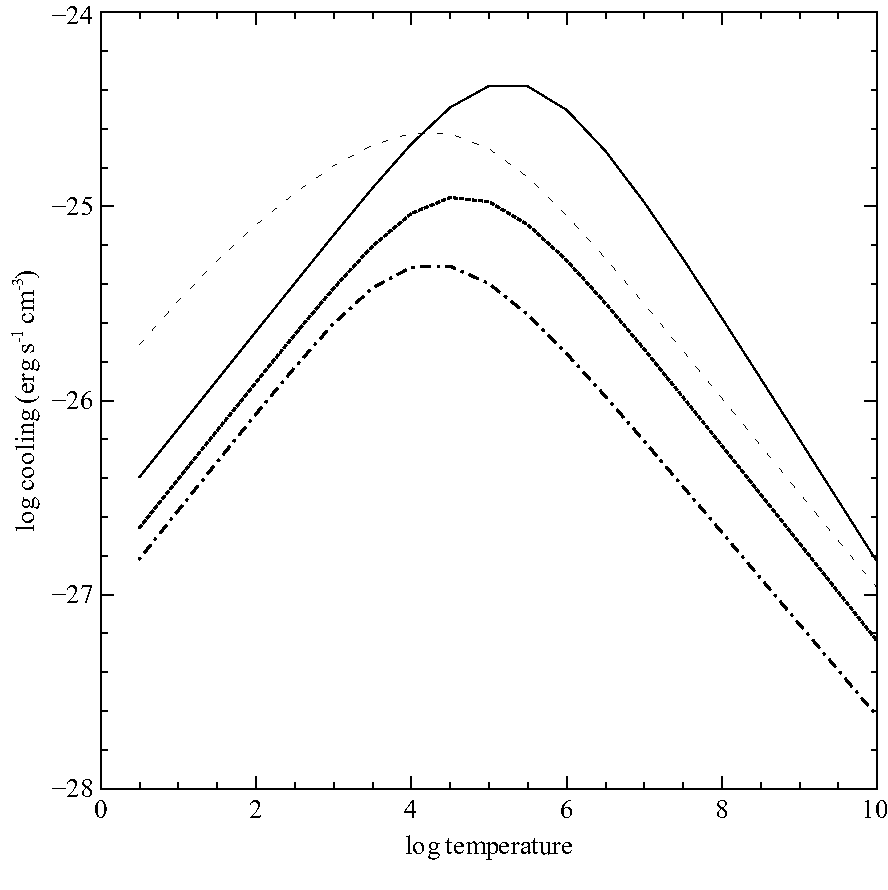
\includegraphics[scale=0.8]{FreeFreeGauntFactors}
\caption[free-free gaunt factors]
{\label{fig:FreeFreeGauntFactors}Thermally averaged
free-free gaunt factor.  The gaunt factor is
shown as a function of photon energy and temperature.}
\end{figure}

\subsection{Bound-free opacity}

Continuum optical depths for photoabsorption from level l are given by
\begin{equation}
d{\tau _l}\left( \nu  \right) = {\alpha _\nu }\left( n
\right)\;{n_l}\,\left[ {1 - \exp \left( { - h\nu /kT} \right)/{b_l}}
\right]\;f(r)\;\delta r% (13)
\end{equation}
where $b_l$ is the departure coefficient for level $l$ and $\alpha _\nu$ is the absorption
cross section [cm$^{-2}$].

\subsection{Plasma frequency}

The plasma frequency, the energy where the index of refraction of an
ionized medium goes to zero, is given by
\begin{equation}
{\nu _{pl}} = {\left( {\frac{{{n_e}q_e^2}}{{\pi \,{m_e}}}} \right)^{1/2}}
= 8.978 \times {10^3}\,n_e^{1/2}\;{s^{ - 1}} = 2.729 \times {10^{ -
12}}\;n_e^{1/2}\;{\mathrm{Ryd}}%. (14)
\end{equation}
An ionized gas will reflect the incident continuum for energies smaller
than this.  This shielding becomes important for the energy range considered
by \Cloudy\ for electron densities greater than $\sim 10^7 \mathrm{cm}^{-3}$.  For higher densities
this process is treated by setting the intensity of the incident continuum
to zero for energies below the plasma frequency, adding this portion of
the incident continuum to the reflected continuum, and not allowing emission
or absorption for any processes that occur below the plasma frequency.

\subsection{Pressure lowering of ionization potential}

The electric field of nearby charges in the continuum acts to lower the
ionization potential.  The amount by which it is lowered is determined by
the electron density.
Ryan Porter extended the code to consider all species
treated with the iso-electronic model atoms.
\section{Continuum range}

The energy interval \emm\ $-$ \egamry\ is divided into a
large number of energy cells with nearly logarithmically increasing widths.

\section{The continuum mesh}

\subsection{Continuum mesh logic}

The central frequencies of two cells are related by
\begin{equation}
\frac{{{\nu _{i + 1}}}}{{{\nu _i}}} = \exp(r)% (100)
\end{equation}
where $r$ is the resolution, $\delta \nu/\nu$.
Then the $n^{th}$ cell energy is related to
the first cell energy by
\begin{equation}
{\nu _n} = {\nu _0}\,\exp(nr).% (101)
\end{equation}
The cell corresponding to energy $\nu_n$ is then
\begin{equation}
n = \frac{\log(\nu_n/\nu_0)}{r}.
\end{equation}

\subsection{Defining the continuum energy mesh}

The array \cdVariable{anu} gives the energy of the center of each
continuum cell, in Rydbergs.
This energy scale is defined in routine
\cdRoutine{ContCreatePointers}.

\subsection{Changing the energy resolution of the mesh}

The file \cdFilename{continuum\_mesh.ini} contains ordered pairs
of continuum energies
and resolving powers (defined as $1/r$) that are read by \cdRoutine{ContCreatePointers}
to set the continuum
mesh when calling \cdRoutine{fill}.
Change the contents of
\cdFilename{continuum\_mesh.ini} to change
the resolution of the continuum mesh.
The file explains how to do this.

If the energy resolving power is increased then the code will require more
mesh points to cover the full continuum and will run more slowly, but the
predicted continuum will have greater detail.

\section{Continuum generation}

The continuum is generated by the function \cdRoutine{ffun}.
\cdRoutine{ffun} has a single argument,
the energy in Rydbergs, and it returns the number of photons per
unit area, time, and Rydberg, at that energy.
\cdRoutine{ffun} sums over all the
specified continua and applies the appropriate normalization factors.
Another function, \cdRoutine{ffun1},
evaluates each individual continuum, and is normally
called only by \cdRoutine{ffun}.

The units, and their conversion to other measures of the continuum, are
given below.  The photon flux density is:
\begin{equation}
{\varphi _\nu }(\nu ) = \mathrm{ffun}(\nu )\quad [\mathrm{photons\,
cm}^{-2} \, \mathrm{s}^{-1} \, \mathrm{Ryd}^{-1}] .
\end{equation}
This is stored in the photon array:
\begin{equation}
flux({\nu _i}) = {\varphi _\nu }(\nu )\;\delta {\nu _i} = \mathrm{ffun}({\nu _i})
\times widflx(\nu )\quad [\mathrm{photons\, cm}^{-2}\, \mathrm{s}^{-1}]
\end{equation}
where \cdVariable{widflx} is an array containing the width of
each continuum bin.
Finally, the energy flux density is given by
\begin{equation}
{f_\nu }(\nu ) = {\mathrm{ffun}}(\nu )\;h\left( {\frac{\nu }{{{\nu _{912}}}}}
\right)\quad
 [\mathrm{erg\, cm}^{-2}\, \mathrm{s}^{-1}\, \mathrm{Hz}^{-1}]
\end{equation}
and
\begin{equation}
\nu {f_\nu }(\nu ) = {\mathrm{ffun}}(\nu )\;h\left( {\frac{\nu }{{{\nu
_{912}}}}} \right){\nu _{912}}\,h{\nu _{Ryd}}\quad
[\mathrm{erg\, cm}^{-2}\, \mathrm{s}^{-1}].
\end{equation}

\section{Energy units; the Rydberg}

Continuum energies are usually given in Rydbergs.
The energy of level
$n$ of a hydrogenic atom is given~by
\begin{equation}
{E_n} =  - \frac{{\cal R}_{\mathrm{H}}}{{{n^2}}}, n = 1,2,3,\ldots,\quad [\mathrm{units\ of\
}\mathcal{R}_{\mathrm{H}}]
\end{equation}
where the Rydberg energy is given by
\begin{equation}
{\cal R} = \frac{{\mu q_e^4}}{{2{\hbar ^2}}} = \frac{\mu }{{{m_e}}}{{\cal
R}_\infty }
\end{equation}
and the reduced mass of the orbiting electron $\mu$ is related
to the electron
and nuclear mass $m_e$ and $m_{nuc}$ by
\begin{equation}
\mu  = \frac{{{m_e}{m_{nuc}}}}{{{m_e} + {m_{nuc}}}} = \frac{{{m_e}}}{{1
+ {{{m_e}} /{{m_{nuc}}}}}}\quad  [\mathrm{g}],% (109)
\end{equation}
(\citealp{Friedrich1998}).
Note that as ${m_{nuc}} \to \infty $, $\mu  \to {m_e}$.
This Rydberg energy $\cal{R}_{\mathrm{H}}$ is smaller than
the energy for an infinite mass
nucleus $\cal{R}_\infty$  by the ratio $\mu/m_e$.
Using the 1998 CODATA revision of the
fundamental constants (see \citealp{Cohen1987,Mohr1998}) the
infinite mass Rydberg energy is given by
\begin{equation}
{{\cal R}_\infty } = \frac{{{m_e}q_e^4}}{{2{\hbar ^2}}} = 13.605698
  [\mathrm{eV}]
\end{equation}
and
\begin{equation}
\begin{array}{c}
 {{\cal R}_\infty }/\left( {2\pi \hbar c} \right) =
109737.315686\;{\mathrm{c}}{{\mathrm{m}}^{ - 1}} \\
 {{\cal R}_\infty }/\left( {2\pi \hbar } \right) = 3.28984196038 \times
{10^{15}}\;{\mathrm{Hz}} \\
 \left( {2\pi \hbar c} \right)/{{\cal R}_\infty } = 91.126732\;{\mathrm{nm}} \\
 \end{array}.
\end{equation}
The ionization potential of hydrogen $\cal{R}_{\mathrm{H}}$ is  $\mu/m_e$ or
$\sim 0.99946$ times
smaller than $\cal{R}_\infty$.
\footnote{$\cal{R}_{\mathrm{H}}$ was the Rydberg unit used by \Cloudy\ before 1988.}
We have
\begin{equation}
\begin{array}{c}
{\cal{R}_{\mathrm{H}}} = 13.59842\;\eV\\
{\cal{R}_{\mathrm{H}}} = 2.178728\times 10^{11}\;\erg\\
\left( 2\pi \hbar\right)/{\cal{R}_{\mathrm{H}}} = 91.176430\;{\mathrm nm}\\
{\cal{R}_{\mathrm{H}}} = 109677.576\;{\mathrm cm}^{-1}
\end{array}
\end{equation}
The difference between $\cal{R}_{\mathrm{H}}$ and $\cal{R}_\infty$ is
significant since it enters as the third
power in the photon phase-space conversion factor $2h \nu^3/c^2$.

The Bohr radius is for an infinite mass nucleus is given by
\begin{equation}
\begin{array}{l}
 {a_o} = {{{\hbar ^2}}/
\left( {{m_e}q_e^2} \right)} = 0.5291772083
\times {10^{ - 8}} \\
 a = {{{a_o}} /\mu } \\
 \end{array}[\mathrm{cm}].
\end{equation}
In the ``atomic units'' system of measuring quantities lengths are given
in terms of the Bohr radius and energies in ``Hartree'' units.  One Hartree
is twice the Rydberg energy.
     %proof 2
\chapter{LINE ATOMIC PARAMETERS}
% !TEX root = hazy2.tex

\section{Overview}

Many atomic physics quantities describe how matter and light interact.
This section goes over these quantities and how they are related to one
another.
The inter-relations between these quantities are described in most
spectroscopy texts, at about the same depth as is given below.  \citet{Hilborn1982} gives a far more formal description,
often tracing quantities back
to basic E\&M concepts.  Highly recommended.

\section{Spectroscopic notation}

A great deal of confusion exists over the difference between the
designation of a spectrum and an ion.  ``Atom~II'' denotes a spectrum, a
collection of photons, while ``Atom$^+$'' denotes a baryon,
the element ``Atom'' with a single electron removed.

Much of the notation in today's atomic physics was developed in the second
half of the 19th century.
Physicists noticed that the spectrum of a gas
would change dramatically when it was heated to high temperatures.
They
did not understand the reason why this happened,
the electron had not yet been discovered,
but they developed the
notation that ``Atom~I'' was the normal spectrum,
this spectrum changed
to ``Atom~II'' when the gas was heated,
and became the ``Atom~III'' spectrum if heated still further.
The ``Atom~II'' spectrum was often called the
``enhanced'' spectrum of Atom.
This is the reason why, in classical novae,
the appearance of broad absorption lines of singly ionized species
is called
the ``diffuse enhanced phase''.

The electron was discovered well after this notation had been developed.
By the early 20th century it was understood that the ``I'' spectrum was
produced by the atom, Atom$^0$.
At high temperatures the first ion, Atom$^+$,
formed and produced the ``Atom~II'' spectrum.

During the first half of the 20th century astrophysicists mainly studied
stellar absorption lines.
This led to the commonly-used notation that the
``Atom~II'' spectrum, for instance, measured Atom$^+$.
It is unambiguously true
that the equivalent width of an Atom~II absorption line is proportional
to the column density of Atom$^+$.
However there is an ambiguity in emission
lines.
The \la\ \hi\ line can be produced by impact excitation
of \hO\ or by recombination of \hplus.
In both cases the line is an \hi\ line, but \hi\ is
produced by either \hO\ or \hplus, depending on details.

To be unambiguously correct you should refer to Atom~I or Atom~II when
discussing the spectrum.
When discussing a column density or particle
density you should refer to the ion, as in Atom$^0$ or Atom$^+$.
It is not correct
to refer to the column density of \hi.
The \la\ \hi\  emission
line measures the column density of either \hO\ or \hplus,
depending on whether the line forms by impact excitation or recombination.
The notation is not ambiguous in absorption lines, which is probably why
we have such confusion today.
Be unambiguous and correct - use the right notation!

\section{Line absorption }

\subsection{Line optical depths}

The optical depth for a transition $u-l$,  where $u$ and $l$ are the upper
and lower levels, is given by
\begin{equation}
\label{eqn:OpticalDepthIncrement}
d{\tau _{l,u}} = {\alpha _\nu }\left( {{n_l} - {n_u}{g_l}/{g_u}}
\right)\;f(r)\;dr
 [\mathrm{Napier}].
\end{equation}
Here $f (r)$ is the filling factor and $\alpha _\nu$ is the
atomic absorption cross section [cm$^2$].

The term in parenthesis is the population [cm$^{-3}$] of the lower level,
with a correction for stimulated emission.
This term is the only place where
stimulated emission enters in the radiative balance equations (\citealp{Elitzur1983}).

\subsection{Oscillator strengths}

The oscillator strength $f$ is a dimensionless number of order unity that
can be thought of as a correction factor to make the expression for a
classical oscillator agree with the quantum mechanical value.
Sections
below relate the oscillator strength to other line parameters such as the
absorption coefficient and the transition probability.
The absorption
($f_{abs}$,
called $f_{l,u}$ here) and emission ($f_{em}$, called $f_{u,l}$)
oscillator strengths are related~by
\begin{equation}
{g_l}{f_{l,u}} =  - {g_u}{f_{u,l}}% (2)
\end{equation}
where the $g$'s are the statistical weights.
This product is symmetric,
neglecting sign, and the code tries to use $gf$'s throughout.
The convention
is that emission lines have negative oscillator strength.

\subsection{Absorption cross section}

The line-center absorption cross section [$\scm$] is related to the
dimensionless absorption oscillator strength $f_{lu}$ or $f_{abs}$ by
\begin{equation}
\label{eqn:LineAbsorptionCrossSection}
\begin{array}{ccl}
 {\alpha _\nu }& =& \frac{{{\pi ^{1/2}}q_e^2\lambda
\,{f_{l,u}}}}{{{m_e}c{u_{Dop}}}}{\varphi _\nu }(x) \\
& =& 0.014974{f_{l,u}}\frac{{{\lambda _{cm}}}}{{{u_{Dop}}}}{\varphi _\nu
}(x) = 1.4974 \times {10^{ - 6}}{f_{l,u}}\frac{{{\lambda _{\mu
m}}}}{{{u_{Dop}}}}{\varphi _\nu }(x) \\
 \end{array}
\quad [\mathrm{cm}^2]
\end{equation}
with the relative line displacement given by
\begin{equation}
\label{eqn:RelativelineDisplacement}
x \equiv \frac{{\nu  - {\nu _o}}}{{\Delta {\nu _{Dop}}}} ,
\end{equation}
${\varphi _\nu }\left( x \right)$
is the Voigt function, and $u_{Dop}$ is the Doppler velocity width
(cm~s$^{-1}$), the
point where the line profile falls to 1/e of its peak.
With this definition
of the relative line displacement, the line profile due to thermal motions
alone is $exp(-x^2)$.
Equation \ref{eqn:LineAbsorptionCrossSection} is evaluated
in routine \cdRoutine{abscf}.

\section{The line profile function}

\subsection{Velocities in a thermal distribution}

The distribution function for a Maxwellian velocity distribution is
given by
\begin{equation}
\frac{{n\left( u \right)du}}{n} = \frac{1}{{{\pi ^{3/2}}}}\exp \left[
{ - {{{u^2}{m_A}} /
{2kT}}}
\right]{\left( {\frac{m}{{2kT}}}
\right)^{3/2}}4\pi {u^2}\,du\quad [\mathrm{cm~s}^{-1}]
\end{equation}
(\citealp{Novotny1973}; p 122).
There are three mean speeds in a thermal velocity
distribution.  The \cdTerm{most probable speed} is the peak
of the velocity
distribution, with a value
\begin{equation}
u_{mean}^2 = 2kT/{m_A}\quad[\mathrm{cm}^2 \; \mathrm{s}^{-2}].
\end{equation}
This is found by setting the derivative of the distribution function to
zero (\citealp{Novotny1973}, p 122).
The velocity distribution function can be
expressed in terms of the \cdTerm{mean speed} as
\begin{equation}
\frac{{n\left( u \right)du}}{n} = \frac{1}{{{\pi ^{3/2}}}}\exp \left[
{ - {{{u^2}} /{u_{mean}^2}}}\right]\frac{{4\pi
{u^2}}}{{u_{mean}^3}}\,du\quad [\mathrm{cm~s}^{-1}].
\end{equation}
The \cdTerm{average speed} is obtained by averaging over this function
and is given by
\begin{equation}
u_{average}^2 =8kT/\pi\, m_A\quad [\mathrm{cm}^2 \; \mathrm{s}^{-2}].% (8)
\end{equation}
The \cdTerm{thermal Doppler velocity width} is the
velocity averaged over the
projected line of sight, given by (\citealp{Novotny1973}; p 204)
\begin{equation}
u_{th}^2 = 2kT/{m_A}
\quad [\mathrm{cm}^2 \; \mathrm{s}^{-2}].
\end{equation}
This is the distance from line center where the line profile
falls to $e^{-1}$ of its central value.
So it turns out that the most probable speed is equal
to the Doppler velocity width.

The \cdTerm{velocity dispersion} $\sigma$ is
\begin{equation}
\sigma  = u/\sqrt 2
\quad [\mathrm{cm~s}^{-1}]% (10)
\end{equation}
and appears in the Gaussian profile function as
\begin{equation}
\varphi \left( {\delta u} \right) = \exp \left( { -
{\raise0.7ex\hbox{${\delta {u^2}}$} \!\mathord{\left/
 {\vphantom {{\delta {u^2}} {2{\sigma ^2}}}}\right.\kern-\nulldelimiterspace}
\!\lower0.7ex\hbox{${2{\sigma ^2}}$}}} \right).% (11)
\end{equation}

\subsection{Micro vs macro turbulence}

Micro-turbulence (hereafter, just turbulence) is due to any additional
motions that occur over scales that are smaller than a photon mean free
path.
Micro-turbulence changes the line transfer since the line opacity
is distributed over a broader range of velocities.
Macro-turbulence is
due to motion that occurs over such large scale lengths that they not change
the optical depth through the emitting region.
An example might be cloud
orbital motions.
The transfer within a cloud is not changed by its bulk
motion and so would be considered macro-turbulence.

\subsection{Line Widths}

If a non-thermal micro-turbulent component of motions is present then
equation \ref{eqn:LineAbsorptionCrossSection},
the total Doppler velocity width [cm~s$^{-1}$] including turbulence,
is given by
\begin{equation}
u_{tot}^2 = 2kT/{m_A} + u_{turb}^2
\quad[\mathrm{cm}^2 \; \mathrm{s}^{-2}]
\end{equation}
as determined by the local kinetic temperature $T$.
Within the code the
micro-turbulent velocity $u_{turb}$ is assumed to be zero
unless it is reset
with the \cdCommand{turbulence} command.\footnote{Note that the
\cdCommand{turbulence} command accepts $u_{turb}$ in $\kmps$ but converts
it into $\cmps$, the units used throughout the code.}

In \cdRoutine{GetDopplerWidth} the Doppler velocity width is evaluated as
\begin{equation}
{u_{Dop}} = \sqrt {2kT/{m_A} + u_{turb}^2}  = \sqrt {1.651 \times
{{10}^8}\,T/{m_{AMU}} + u_{turb}^2}
\quad  [\cmps].
\end{equation}
The atomic weight is in atomic mass units.

The Doppler velocity width is related to the half width at half maximum
by (\citealp{Novotny1973}, eqns 5-18; p 205)
\begin{equation}
\Delta {u_{1/2}} = {\left( {\ln 2} \right)^{1/2}}{u_{Dop}} =
0.832555\,{u_{Dop}}
\quad  [\mathrm{cm~s}^{-1}]
\end{equation}
and the FWHM is given by
\begin{equation}
\Delta {u_{FWHM}} = 2{\left( {\ln 2} \right)^{1/2}}{u_{Dop}}
\quad [\mathrm{cm~s}^{-1}].
\end{equation}

\subsection{The Doppler $b$ parameter}

Much of the literature refers to the Doppler $b$ parameter.
This is the
Doppler velocity width or velocity dispersion with turbulence included,
and is given by
\begin{equation}
{b^2} = u_{Dop}^2 = 2kT/{m_A} + u_{turb}^2
\quad [\mathrm{cm}^2 \mathrm{s}^{-2}].
\end{equation}
With these definitions
\begin{equation}
b = {u_{Dop}} = \Delta {u_{FWHM}}/\left[ {2{{\left( {\ln 2} \right)}^{1/2}}}
\right]
\quad  [\mathrm{cm~s}^{-1}].
\end{equation}

\subsection{Voigt function}

Optical depths a relative displacement $x$ away from line center
are related
to the line center optical depth $\tau_0$ by
\begin{equation}
\tau (x)=\tau_0 \varphi_\nu (x).% (18)
\end{equation}
The relative displacement is given by
equation \ref{eqn:RelativelineDisplacement} above.
The Voigt function
is normalized to unity at line center and is approximately given by
\begin{equation}
\label{eqn:VoigtFunctionApproximation}
{\varphi _\nu }(x) \approx \exp ( - {x^2}) + a/({\pi ^{1/2}}{x^2}) .
\end{equation}
Here $a$ is the damping constant and the expression is valid only
for small $a$.
At line center 
${\varphi _\nu }\left( {a,x} \right) \sim \left( {1 + a} \right)^{ - 1}$,
while the core of the line is roughly $x \sim \left( {1 + a} \right)$ wide.
The line center optical depth thus depends on $a$ when $a\geq 1$,
while the mean optical depth is constant.

\subsection{Mean vs. line center optical depths}

\Cloudy\ works with line center optical depths throughout (see,
for example, \citealp{Mihalas1978}).
However, mean optical depths are reported in the final printout.
For comparison, the line
center optical depth is $\pi^{1/2}$ times \emph{smaller} than
the mean optical depth when the damping constant $a$ is small, $a\ll1$.

In many places routines or approximations using
\emph{mean} optical depths are encountered
(e.g., \citealp{Hummer1980}).
The difference is in how
equation \ref{eqn:VoigtFunctionApproximation} is normalized.

\section{The Einstein coefficients}

The dimensionless oscillator strength $gf$ is related to the transition
probability $A_{ul}$ [s$^{-1}$]~by
\begin{equation}
{g_l}{f_{l,u}} = {g_u}{f_{u,l}} = \frac{{{m_e}c\lambda _{cm}^2}}{{8{\pi
^2}q_e^2}}{g_u}{A_{u,l}} = 1.4992{g_u}{A_{u,l}}\lambda _{cm}^{\,2} = 1.4992
\times {10^{ - 8}}{g_u}{A_{u,l}}\lambda _{\micron}^{\,2}
\end{equation}
where $\lambda_{\micron}$ is the wavelength in microns and $\lambda_{cm}$ the wavelength in centimeters.
The absorption oscillator strength is related to the
transition probability by
\begin{equation}
\label{eqn:gfAulRelation}
{f_{l,u}} = \frac{{{m_e}c\lambda _{cm}^2}}{{8{\pi
^2}q_e^2}}\frac{{{g_u}}}{{{g_l}}}{A_{u,l}} = 1.4992 \times {10^{ -
8}}{A_{u,l}}\lambda _{\mu m}^{\,2}\frac{{{g_u}}}{{{g_l}}}
\end{equation}
or
\begin{equation}
{A_{u,l}} = \frac{{8{\pi ^2}q_e^2}}{{mc\lambda
_{cm}^2}}\frac{{{g_l}}}{{{g_u}}}{f_{abs}} = \frac{{{f_{l,u}}}}{{1.4992 \times
{{10}^{ - 8}}}}\lambda _{\mu m}^{ - \,2}\frac{{{g_l}}}{{{g_u}}}\quad
[\mathrm{s}^{-1}].
\end{equation}
Combining equations \ref{eqn:LineAbsorptionCrossSection}
and \ref{eqn:gfAulRelation} we obtain an expression relating the
transition probability and the absorption cross section;
\begin{equation}
\begin{array}{ccl}
 {\alpha _\nu }& =& \frac{{{\lambda ^3}{g_u}}}{{8\pi
{g_l}}}\frac{{{A_{u,l}}}}{{{\pi ^{1/2}}{u_{Dop}}}}{\varphi _\nu }\left(
x \right) \\
&=& \frac{{{\lambda ^3}{g_u}}}{{8\pi {g_l}}}\frac{{{A_{u,l}}}}{{{\pi
^{1/2}}{u_{Dop}}}}{\varphi _\nu }\left( x \right) \\
&=& 2.24484 \times {10^{ - 14}}{A_{u,l}}\lambda _{\mu
m}^{\,3}\frac{{{g_u}}}{{{g_l}}}\frac{{{\varphi _\nu }\left( x
\right)}}{{{u_{Dop}}}} \\
 \end{array}
\quad  [\mathrm{cm}^2].
\end{equation}
The coefficient for induced emission,
$B_{ul}$, is related to $A_{ul}$ by the phase
space factor $2h{\nu ^3}/{c^2}$;
\begin{equation}
{A_{u,l}} = \frac{{2h{\nu ^3}}}{{{c^2}}}{B_{ul}}
\quad [\mathrm{s}^{-1}]
\end{equation}
and the induced emission and absorption probabilities are related by
\begin{equation}
{g_l}{B_{l,u}} = {g_u}{B_{u,l}}
\end{equation}
The absorption cross section $\alpha _v$ is related to $B_{l,u}$ by
\begin{equation}
{\alpha _\nu }\, = \frac{{hc}}{{4{\pi
^{3/2}}}}\frac{{{B_{l,u}}}}{{{u_{Dop}}}}{\varphi _\nu }\left( x \right)
\quad [\mathrm{cm}^2].
\end{equation}
In these terms the optical depth increment
(equation \ref{eqn:OpticalDepthIncrement}) is given by
\begin{equation}
\begin{array}{ccl}
 d{\tau _{l,u}}& =& {\alpha _\nu }\left( {{n_l} - {n_u}{g_l}/{g_u}}
\right)f\left( r \right)\,\,dr \\
& =& \frac{{hc}}{{4{\pi ^{3/2}}}}\frac{{{B_{l,u}}}}{{{u_{Dop}}}}{\varphi
_\nu }\left( x \right)\left( {{n_l} - {n_u}{g_l}/{g_u}} \right)f\left( r
\right)\,dr \\
 \end{array}
 .
\end{equation}

\section{Continuum pumping}

\subsection{Photon occupation number}

The intensity of a radiation field can be thought of as two parts, the
available volume of phase space $2h{\nu ^3}/{c^2}$
and a dimensionless occupation number $\eta$ giving the fraction
of that space that is filled.
Occupation numbers can be larger than unity for
photons, which are Bose-Einstein particles.

For reference, the Planck function is given by
\begin{equation}
{B_\nu } = {I_\nu } = \frac{{{F_\nu }}}{\pi } = \frac{{2h{\nu
^3}}}{{{c^2}}}\frac{1}{{\exp \left( {h\nu /kT} \right) - 1}}
\quad  [\mathrm{erg~cm}^{-2}\;\mathrm{s}^{-1}\; \mathrm{sr}^{-1}\; \mathrm{Hz}^{-1}]% (28)
\end{equation}
where $F_\nu$ is the single-hemisphere emittance from an opaque surface.
The photon occupation number of a blackbody is then
\begin{equation}
\label{eqn:PhotonOccupationNumber}
{\eta _\nu } = \frac{1}{{\exp \left( {h\nu /kT} \right) - 1}}
\end{equation}
The dimensionless occupation number for any continuum with a mean intensity
$J_\nu$ (erg~cm$^{-2}$~s$^{-1}$~Hz$^{-1}$ sr$^{-1}$) at a frequency $\nu$ is defined as
\begin{equation}
{\eta _\nu } \equiv {J_\nu }/\left( {2h{\nu ^3}/{c^2}} \right) \equiv
{\left[ {\exp \left( {h\nu /k{T_{ex}}} \right) - 1} \right]^{ - 1}}
.
\end{equation}
Here $T_{ex}$ is the excitation temperature of the continuum at the frequency.

\subsection{Pumping rates}

Continuum fluorescence is treated as in \citet{Ferland1988} and \citet{Ferland1992}.
The rate of induced radiative excitation by continuum photons
(continuum pumping) is given by
\begin{equation}
{r_{l,u}} = {n_l}{B_{l,u}}{J_{l,u}} =
{n_l}{A_{u,l}}\frac{{{J_{l,u}}}}{{2h{\nu ^3}/{c^2}}}\frac{{{g_u}}}{{{g_l}}}
= {n_l}{A_{u,l}}{\eta _\nu }\frac{{{g_u}}}{{{g_l}}}
\quad [\mathrm{cm}^{-3}\;\mathrm{s}^{-1}]
\end{equation}
where $\eta_\nu$ is the dimensionless continuum occupation number
at the line energy.
The rate of induced radiative de-excitation is related by
detailed balance and is given by
\begin{equation}
{r_{u,l}} = {r_{l,u}}\frac{{{g_l}}}{{{g_u}}}
\quad [\mathrm{cm}^{-3} \;\mathrm{s}^{-1}].
\end{equation}
The occupation number has the advantage that the Einstein $B$'s
do not enter any rate equations.
All radiative rates can be expressed in terms of an
$A$ and $\nu$.

\subsection{Optical depth effects}

The line becomes self-shielding when the optical depth is greater than
unity.
The line optical depth between the current position and the
illuminated face of the slab is used to evaluate the inward-looking escape
probability, the probability that a line photon will travel this distance
in a single scattering.
Line optical depths do not directly affect $\eta_c$,
only continuous opacities do.
The final form of the continuum pumping rate is
\begin{equation}
{r_{l,u}} = {n_l}{A_{u,l}}{\eta _\nu }\frac{{{g_u}}}{{{g_l}}}{\gamma
_{l,u}}\left( \tau  \right)
\quad [\mathrm{cm}^{-3} \;\mathrm{s}^{-1}]
\end{equation}
where $\gamma_{l,u}$ is the probability that continuum photons
penetrate an optical
depth $\tau_o$ and are then absorbed by an atom:
\begin{equation}
{\gamma _{l,u}} = \int_0^\infty  {{\varphi _\nu }\;\exp \left( { - {\tau
_o}{\varphi _\nu }} \right)\,d\nu } /\int_0^\infty  {{\varphi _\nu }\;d\nu
} .
\end{equation}
where $\varphi_\nu$ is the Voigt function.
Figure \ref{fig:pump_probability},
taken from \citet{Ferland1992}, shows
$\gamma_{l,u}$ for a wide variety of values of the damping constant $a$.

\begin{figure}
\centering
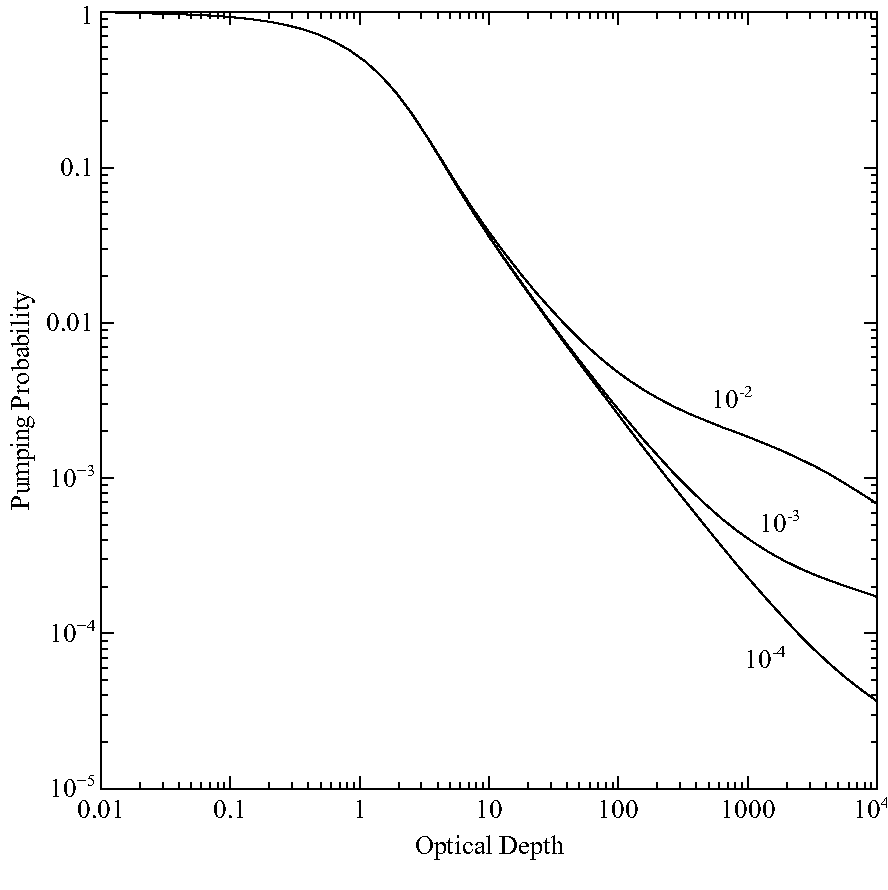
\includegraphics[scale=0.8]{pump_probability}
\caption[Fluorescent pumping probability]{\label{fig:pump_probability}This figure
shows the probability that a photon will penetrate
to the line center optical depth shown on the x-axis, and then be absorbed
by the line.  The curves are for various values of the damping constant
a (the ratio of damping width to Doppler width), as indicated on the
figure.}
\end{figure}

The code works in terms of the flux of photons per energy mesh point.
The transmitted continuum has a flux of photons $\varphi_\nu$
(photons cm$^{-2}$ s$^{-1}$ Ryd$^{-1}$).
The photon occupation number of the attenuated continuum is given by equation \ref{eqn:PhotonOccupationNumber} above, here written as
\begin{equation}
{\eta _\nu } = {\varphi _\nu }\;\frac{{{c^2}}}{{8\pi \;\nu _1^3\;\nu
_{Ryd}^2}}
\end{equation}
where $\nu_{Ryd}$ is the frequency in Rydbergs,
$\nu_1$ is the frequency of 1 Rydberg,
and the other symbols have their usual meaning.
Continuum pumping is
included among the general line excitation processes for all lines
considered by the code.

\section{Kirchhoff's Law}

Kirchhoff's law is the statement that, in thermodynamic equilibrium,
the energy emitted is equal to the energy absorbed.  If the emission and
absorption coefficients are $j_{\nu}$ and $\kappa_{\nu}$ then
\begin{equation}
j_{\nu} = \kappa_{\nu} B_{\nu}(T)
\end{equation}
where $B_{\nu}(T)$ is Planck's function.

\section{The line source function and mean intensity}

The source function for a line is defined as
\begin{equation}
{S_l}\left( {{T_{exc}}} \right) \equiv {B_l}\left( {{T_{exc}}} \right)
\equiv \frac{{{j_l}}}{{{\kappa _l}}} =
\frac{{{A_{u,l}}{n_u}}}{{{B_{l,u}}\left( {{n_l} - {n_u}{g_l}/{g_u}}
\right)}}
\quad
  [\mathrm{erg~Hz}^{-1}\; \mathrm{sr}^{-1}\; \mathrm{s}^{-1}].
\end{equation}
where $T_{exc}$ is the line excitation temperature
\begin{equation}
\frac{{{n_u}/{g_u}}}{{{n_l}/{g_l}}} = \exp \left[ { - h\nu /k{T_{exc}}}
\right]
\end{equation}
$B_l(T_{exc})$ is the Planck function at the line excitation
temperature and the
line emission and absorption coefficients $jl$ and $kl$
enter through Kirchhoff's law.
Combining with the definitions of the Einstein relations we find the
relation
\begin{equation}
{S_l}\left( {{T_{exc}}} \right) = \frac{{2h{\nu
^3}}}{{{c^2}}}\frac{{{n_u}/{g_u}}}{{\left( {{n_l}/{g_l} - {n_u}/{g_u}}
\right)}}
\quad  [\mathrm{erg~Hz}^{-1}\; \mathrm{sr}^{-1}\; \mathrm{s}^{-1}].
\end{equation}
The radiation field within the line is given by the mean intensity
$\bar J$.
$\bar J$  and $S_l$ are related by the net radiative bracket,
which we approximate as
the escape probability $P_{esc}$:
\begin{equation}
{P_{esc}} \equiv 1 - \bar J/{S_l}. %(40)
\end{equation}
The mean intensity is then give by
\begin{equation}
\bar J = {S_l}\left( {1 - {P_{esc}}} \right) .% (41)
\end{equation}
and the line center photon occupation number is
\begin{equation}
{\eta _l} = \frac{{{n_u}/{g_u}}}{{\left( {{n_l}/{g_l} - {n_u}/{g_u}}
\right)}}\left( {1 - {P_{esc}}} \right).
\end{equation}

\section{Level populations in radiative equilibrium limit}

For a two-level system where collisions can be neglected, in the optically
thin limit, the balance equation relating the populations of a two-level
system is given by
\begin{equation}
\frac{{d{n_u}}}{{dt}} = {n_l}{B_{lu}}J - {n_u}\left( {{A_{ul}} + {B_{ul}}J}
\right)
\quad  [\mathrm{cm}^{-3} \;\mathrm{s}^{-1}].
\end{equation}
In the time-steady limit, where the time derivative is zero, the balance
can be rewritten in terms of the transition probabilities as
\begin{equation}
{n_u}\left( {{A_{ul}} + {A_{ul}}\eta } \right) = {n_u}{A_{ul}}\left( {1
+ \eta } \right) = {n_l}{A_{ul}}\eta \frac{{{g_u}}}{{{g_l}}}
\quad  [\mathrm{cm}^{-3} \;\mathrm{s}^{-1}].
\end{equation}
In the limit where $\eta$ is small every photoexcitation is followed by
spontaneous decay, while in the limit where $\eta$ is large the level populations
are given by the ratio of statistical weights, i.e., $T_{exc}$ is infinite.



%proof 1
\chapter{LINE DETAILS }
% !TEX root = hazy2.tex

\section{Overview }

The effects of optical depths, continuum pumping, collisions, and
destruction by background opacity,
are computed for \emph{all} permitted and
intercombination lines.
The cooling is usually distributed among many lines
in high-density models, and these lines are usually optically thick.   This
section describes the methods and data structures used within the code to
accomplish this.

\section{Line Boltzmann factors }

The Boltzmann factor $h\nu/kT$ for a line with a known wavelength or
energy is given by Table \ref{tab:LineBoltzmann}.
The table lists the ratio $h\nu/k$ for various units of
the line energy.
Vacuum, not air, wavelengths, must be used for all
quantities involving wavelengths.

\begin{table}
\centering
\caption{\label{tab:LineBoltzmann}Line Boltzmann Factors }
\begin{tabular}{ll}
\hline
Line Energy Units& $h\nu/k$ (K)\\
\hline
 Angstroms& 1.43877(+8)/$\lambda$(\AA)\\
microns& 1.43877(+4)/$\lambda(\mu)$\\
 wavenumbers& 1.43877$\times \sigma$\\
 Rydbergs& 1.5788866(+5) $\times$E\\
\hline
\end{tabular}
\end{table}

\section{Air vs vacuum wavelengths }

The convention across physics and astronomy is to give line wavelengths
in vacuum for $\lambda\le 2000$~\AA\ and in air for $\lambda > 2000$~\AA.
There is no choice---if you observe visible light with
HST the wavelengths must be quoted in air.

Air wavelengths are smaller than vacuum wavelengths because the wavefronts
are crushed as then enter the denser medium with its higher index of
refraction.
The frequency is unchanged.

\section{The line escape probability functions }

\subsection{Escape probability formalism vs exact radiative transfer }

Radiative transport effects are approximated with the escape probability
formalism (EPF).  This includes line pumping by the incident continuum,
photon destruction by collisional deactivation or by continuous opacities,
and line overlap in special cases.  This section describes how the escape
probability is related to the net radiative bracket, the formally correct
term in the transfer equation.

The full balance equation for radiative losses and gains for the upper
level of a two level atom is given by
\begin{equation}
{n_u}{A_{ul}} + {n_u}{B_{ul}}\bar J - {n_l}{B_{lu}}\bar J \equiv
{n_u}{A_{ul}}{\rho _{ul}} \approx {n_u}{A_{ul}}{P_{ul}}% (1)
\end{equation}
where $A$ and $B$ are the Einstein coefficients, $\bar J$
is the mean intensity averaged over the line,
and $\rho_{\mathrm{ul}}$ is the net radiative bracket, defined as
\begin{equation}
{\rho _{ul}} \equiv 1 - \bar J/S% (2)
\end{equation}
where $S$ is the line source function.
The essence of the EPF is to replace
$\rho_{\mathrm{ul}}$ with the escape probability $P_{ul}$ on the argument that the difference
between $J$ and $S$ is due to photons leaking away from the region.  (\citealp{Elitzur1983}; Sec 2.6) shows that this is exact
if $S$ is constant across the
line-forming region.
In the code $\rho_{\mathrm{ul}}$ is replaced with $P_{ul}$.

\subsection{Redistribution functions }

At low densities, line scattering for a two-level atom is coherent in
the atom's reference frame and the line profile function is described by
the incomplete redistribution function.
At high densities the Stark effect
can broaden the line.
When the radiation density is high, scattering within
excited states can inhibit the broadening of resonance lines such as
L$\beta$ (line
interlocking), destroying the coherence of the scattering process.
In these
cases complete redistribution in a Doppler core more closely describes the
scattering process.

\Cloudy\ uses several escape probability functions to take these processes
into account.
Strong resonance lines are treated with partial redistribution
with a Voigt profile.
Subordinate lines are treated with complete
redistribution in a Doppler core.

\subsection{Incomplete redistribution }

Incomplete redistribution is assumed for resonance transitions such as
C~IV $\lambda$1549 and the \la\ transitions of hydrogen and helium.  Two studies of
line formation using this approximation are those of \citet{Bonihala1979}
and \citet{Hummer1980}.
Both studies suggest escape probabilities of the form
\begin{equation}
{P_l}(\tau ) = {\left\{ {1 + b\left( \tau  \right)\,\tau } \right\}^{
- 1}}% (3)
\end{equation}
but there is substantial disagreement in the form and value of the factor
$b(\tau)$, sometimes by more than a factor of 2.
(This is after due allowance
for the different definitions of line opacities in the two papers.)  \Cloudy\
uses the \citet{Hummer1980} results for \hi, \hei, and \heii\ \la\ and
strong resonance lines such as C~IV $\lambda$1549.
Their tabulated values were fitted
by interpolation.

\subsection{Damping constant }

The damping constant $a$ is given by
\begin{equation}
a = \frac{\Gamma }{{4\pi \;\Delta {\nu _D}}} = \frac{{{\lambda _{cm}}\sum
A }}{{4\pi \,{u_{Dop}}}} = \frac{{{\lambda _{cm}}7.958 \times {{10}^{ -
2}}\sum {A\,} }}{{{u_{Dop}}}} = \frac{{{\lambda _{\mu m}}7.958 \times {{10}^{
- 6}}\sum {A\,} }}{{{u_{Dop}}}}% (4)
\end{equation}
where $\Gamma$ is the inverse lifetime of the level
(the sum of the $A$'s from the
upper level), $\Delta {\nu _D}$
is the Doppler width in frequency units \citep{Mihalas1978},
$\lambda_{cm}$ and $\lambda_{\mu m}$ are
the wavelengths in cm and microns respectively,
and $u_{Dop}$ is the Doppler width in cm~s$^{-1}$.
The ratio $\Gamma \lambda /4\pi $
is stored in the line structures and the $a$'s are evaluated
using this ratio
and the current Doppler width.

\subsection{Background opacity and Destruction probability }

The ratio of continuous to total opacity is $X_c$ parameterized as
\begin{equation}
{X_c} = \frac{{\sum {{\kappa _c}\;{n_c}} }}{{{\kappa _l}{n_l} + \sum
{{\kappa _c}\;{n_c}} }}% (5)
\end{equation}
where the $\kappa_l$'s are the line center absorption opacities and the $n$'s the number
of absorbers.

\subsection{Complete redistribution }

Lines arising from excited states (hydrogen Balmer, Paschen, etc.) and
Lyman lines with $n_u > 2$ are treated assuming complete redistribution in
a Doppler core (i.e., the damping constant $a$ is assumed to be zero).  This
assumption can be changed with the \cdCommand{atom redistribution} command.  If the
total optical depth of the slab is $T$, then the escape probability at a
depth $\tau$
from the illuminated face is given by;
\begin{equation}
{P_{u,l}}(\tau ,\,T,\,{X_c}) = \left[ {1 - {X_c}F({X_c})}
\right]\frac{1}{2}\left[ {{K_2}(\tau ,\,{X_c}) + {K_2}(T - \tau ,\,{X_c})}
\right]\quad ,% (6)
\end{equation}
and the destruction probability is
\begin{equation}
{D_{u,l}}({X_c}) = {X_c}F({X_c}).% (7)
\end{equation}
The function is
\begin{equation}
F({X_c}) = \int_{ - \infty }^\infty  {\frac{{\varphi (x)}}{{{X_c} + \varphi
(x)}}\;dx},% (8)
\end{equation}
where in these expressions (and in this part of the code) the
\emph{mean opacity is used},
and $\varphi(x)\approx \pi^{1/2} \exp(-x^2)$ is the Voigt
function.
$F(X_c)$ is interpolated
from the tables presented by Hummer (1968).
The function
\begin{equation}
{K_2}(\tau ,\,{X_c}) \equiv \frac{1}{{1 - {X_c}F({X_c})}}\int_{ - \infty
}^\infty  {\frac{{{\varphi ^2}(x)}}{{{X_c} + \varphi (x)}}{E_2}\left[ {\left(
{{X_c} + \varphi (x)} \right)\tau } \right]\;d\tau }
\end{equation}
is evaluated numerically.

The complete redistribution escape probabilities are corrected for
finite damping parameters by including a separate wing escape
probability.  The resulting total escape probabilities have been
tested against numerical integrations of the exact formulae in
\cite{Avrett1966,Hummer1982b} -- note the different definitions of
$K_2$ in these papers -- verified by comparison by the tabulations and
fits in these papers.  The overall fit to the escape probability is in
error by at most 25\% in the range $a=10^{-3}\mbox{--}10^3$, with the
largest error at $\tau\simeq 1$, and correct asymptotic behaviour in
the low $\tau$ and high $\tau$ limits.  This level of accuracy is
thought to be sufficient, given the other approximations inherent in
the escape probability method.

\subsection{Masing lines }

A line mases when its optical depth is negative.
The escape probability is (\citealp{Elitzur1992}; p 32)
\begin{equation}
{P_{u,l}} = \frac{{1 - \exp \left( { - \tau } \right)}}{\tau }.% (10)
\end{equation}
The code will generate a comment if strong maser action occurs for any
transition.

\subsection{Stark broadening }

Distant collisions with charged particles broaden the upper levels of
lines, and in the limit of very high densities this will make the scattering
process completely non-coherent even for L$\alpha $ (i.e., complete redistribution
obtains).
Cloudy closely follows the treatment of \citet{Puetter1981} in treating
Stark broadening.

\subsection{Net escape probability }

A total escape probability $P_{l, tot}$, given by
\begin{equation}
{P_{u,l}} = \min \left( {{P_{inc}} + {P_{Stark}}\;,\;{P_{com}}} \right),% (11)
\end{equation}
is defined for transitions described by incomplete redistribution.  The
escape probabilities are those for incomplete, Stark, and complete
redistribution respectively.  The total effective escape probability is
not allowed to exceed the complete redistribution value for
$\tau > a^{-1}$.

If $\tau$ is the optical depth in the direction towards the source of ionizing
radiation and $T$ is the total optical depth computed in a previous iteration,
then the escape probability entering the balance equations is
\begin{equation}
{P_{u,l}}\left( {\tau ,T} \right) = \left\{ {{P_{u,l}}\left( \tau  \right)
+ {P_{u,l}}\left( {T - \tau } \right)} \right\}/2.
\end{equation}
In general the total optical depth $T$ is only known after the first iteration,
so more than one iteration must be performed when radiative transfer is
important.

\section{Optical depths and the geometry }

The terms open and closed geometry are defined in a section in Part I.
The treatment of transfer in these two limits is described here.

\subsection{Open geometry }

This is the default.  During the first iteration the line optical depth
is defined using only optical depths accumulated in the inward direction.
This optical depth is initialized to a very small number at the start of
the calculation.
At the end of the first iteration the total optical depth
is set to the optical depth accumulated in the inward direction.
At the
end of subsequent iterations the total optical depth is defined as a mean
of the new and old inward optical depths.

\subsection{Closed geometry overview }

Continuum photons are assumed to interact with gas fully covering the
continuum source.  At the end of the first iteration the total continuum
optical depths are set equal to twice the computed optical depths, and the
inner optical depths reset to the computed optical depths.
The same recipe
is followed on subsequent iterations, except that means of old and newly
computed optical depths are used.

\cdCommand{Closed expanding geometry}  This is the default if the
\cdCommand{sphere} command
is entered.  In this case it is assumed that line photons do not interact
with lines on the ``other'' side of the expanding spherical nebula.  The
treatment of line optical depths is entirely analogous to that described
for an open geometry, since the presence of the distant material has no
effect on line transfer.

\cdCommand{Closed static geometry}  This is assumed if the \cdCommand{sphere static} command
is entered.
In this case line photons from all parts of the spherical shell
do interact.
As a result the optical depth scale is poorly defined on the
first iteration, and more than one iteration is required.
On second and
later iterations the total line optical depth is set to twice the optical
depth of the computed structure, and the optical depth at the illuminated
face of the shell is set to half of this.
The optical depth scale is only
reliably defined after at least a second iteration.

\subsection{Wind }

The model is a large velocity gradient $(v\propto R$ Sobolev approximation) wind.
This is described further in Part 2 of this document.

\section{Collision strengths }

I have tried to follow the Opacity Project notation throughout this
document \citep{Lanzafame1993}.
The energy-specific collision strength
$\Omega_{lu}$ for a transition between upper and lower levels $u$ and $l$ is related to
the excitation cross section $Q_{lu}$~by
\begin{equation}
{Q_{lu}} = \frac{{\pi {\Omega _{lu}}}}{{glk_{lu}^2}}
\quad [\mathrm{cm}^2]
\end{equation}
where $k_{lu}^2$  is the wavenumber of the collision energy.
If the collisions are with
thermal electrons having a Maxwellian velocity distribution $f(u)$ and velocity
$u$ then the rate coefficient $q_{lu}$ is given by
\begin{equation}
{q_{lu}} = \int_0^\infty  {f\left( u \right)} u{Q_{lu}}\,du = \frac{{2{\pi
^{1/2}}{\hbar ^2}}}{{{g_l}{m_e}}}{a_o}\left( {\frac{{{R_\infty }}}{{kT}}}
\right){\Upsilon _{lu}}\exp \left( { - \frac{{{E_{lu}}}}{{kT}}} \right)\sqrt
{\frac{{2kT}}{{{m_e}}}}\quad
[\mathrm{cm}^3 \mathrm{s}^{-1}].
\end{equation}
$E_{ul}$ is the transition energy in Rydbergs, $a_o$ is the Bohr radius,
\begin{equation}
{a_o} = \frac{{{\hbar ^2}}}{{{m_e}q_e^2}} = 0.529177249 \times {10^{ -
8}}\;{\mathrm{cm}}
\end{equation}
and ${R_\infty }$ is the Rydberg energy.
Then the thermally-averaged collision strength is given by
\begin{equation}
{\Upsilon _{lu}} = \int_0^\infty  {{\Omega _{lu}}\exp \left( { -
\frac{\varepsilon }{{kT}}} \right)\;d\left( {\frac{\varepsilon }{{kT}}}
\right)}.
\end{equation}
The rate coefficient for collisional de-excitation is then given by
\begin{equation}
{q_{ul}} = \frac{\Upsilon }{{{g_u}\sqrt {{T_e}} }}{\left( {\frac{{2\pi
}}{k}} \right)^{1/2}}\frac{{{\hbar ^2}}}{{m_e^{3/2}}} = \frac{{\Upsilon
\,8.6291 \times {{10}^{ - 6}}}}{{{g_u}\sqrt {{T_e}} }}
\quad  [\mathrm{cm}^3 \mathrm{s}^{-1}].
\end{equation}
The rate coefficient for excitation follows from detailed balance:
\begin{equation}
{q_{lu}} = {q_{ul}}\frac{{{g_u}}}{{{g_l}}}\exp \left( { - \chi } \right)
= \frac{{\Upsilon \,8.6291 \times {{10}^{ - 6}}}}{{{g_l}\sqrt {{T_e}} }}\exp
\left( { - \chi } \right)\quad  [\mathrm{cm}^3 \mathrm{s}^{-1}].
\end{equation}

\section{Born approximation }

The Born approximation is valid for energies much larger than the
excitation energy of the transition.
The energy specific collision strength
is given by \citet{Bethe1930} as
\begin{equation}
{\Omega _{lu}} \approx \frac{{4{g_l}{f_{lu}}}}{{{E_{lu}}}}\ln \left(
{\frac{{4\varepsilon }}{{{E_{lu}}}}} \right)
\end{equation}
where $f_{l,u}$ is the absorption oscillator strength of the permitted transition.

\section{The g-bar approximation }

The g-bar or \citet{VanRegemorter1962} approximation relates the collision
strength to the transition probability $A_{ul}$ and wavelength $\lambda$ (in \micron).
Here, the collision strength for the downward transition
${\Upsilon _{ul}}$
is approximately given by
\begin{equation}
\begin{array}{ccl}
 {\Upsilon _{u,l}}& =& \frac{{2\pi }}{{\sqrt 3
}}\frac{{{m^2}{e^2}}}{{{h^3}}}\lambda _{\mu m}^3{10^{ -
12}}{g_u}{A_{u,l}}\bar g \\
& \approx& 2.388 \times {10^{ - 6}}\lambda _{\mu m}^3{g_u}{A_{u,l}}\bar g \\
& \approx& 159{\lambda _{\mu m}}{g_l}{f_{abs}}\bar g \\
 \end{array}
\end{equation}
where $g_u$ and $g_l$ are the statistical weights of the
upper and lower levels
and $f_{abs}$ is the absorption oscillator strength.
For energies of interest
in astrophysical plasmas, where $kT<h\nu$, $\bar g$
is approximately given by
\begin{equation}
\bar g \approx \left\{ {\begin{array}{*{20}{c}}
   \hfill {0.2;} & \hfill {{\mathrm{positive}}\;{\mathrm{ions}}} \\
   \hfill {\left( {{\mathrm{kT/h}}\nu } \right)/10;}\& \hfill {{\mathrm{neutrals}}}
\\
\end{array}} \right.
\end{equation}
(van Regemorter 1962).
These approximations are generally accurate to better
than 1 dex.
\citet{Gaetz1983} give improved forms of the approximation.

\section{The critical density }

The critical density is defined as the density at which the radiative
de-excitation rate $A_{ul}\, P_{ul}$ (where $A$ is the transition
probability and $P$
is the escape probability) equals the collisional de-excitation rate
$q_{ul}n_e$.
Setting
\begin{equation}
{A_{ul}}{P_{ul}} = {C_{ul}} = {q_{ul}}{n_e} = \Upsilon \frac{{8.629 \times
{{10}^{ - 6}}}}{{{g_u}\sqrt {{T_e}} }}{n_e}\quad
  [\mathrm{s}^{-1}]
\end{equation}
where $\Upsilon$ is the thermally averaged collision strength,
the critical density
is given by
\begin{equation}
{n_{crit}} \sim \frac{{{A_{ul}}{P_{ul}}{g_u}\sqrt {{T_e}} }}{{\Upsilon
\,8.629 \times {{10}^{ - 6}}}}\quad
  [\mathrm{cm}^{-3}].
\end{equation}
For an optically allowed transition, in which the g-bar approximation may
apply, this density is approximately given by
\begin{equation}
{n_{crit}} = \frac{{4.8 \times {{10}^{10}}\sqrt {{T_e}} }}{{\lambda _{\mu
m}^3\bar g}}\quad
[\mathrm{cm}^{-3}].
\end{equation}

\section{Line thermalization length }

Line radiative transfer will affect the thermal equilibrium of the gas
when the collision time scale approaches an effective lifetime $\tau\sim
A_{ul} /n_{scat} )^{-1}$, where $A_{ul}$ is the transition probability and
$n_{scat}$ is the number
of scatterings a line photon undergoes before escape.
For permitted metal
lines (which often have optical depths  $\sim10^4 - 10^6$) line thermalization
becomes important at densities $n_e >10^{15} / \tau 10^{10} \mathrm{cm}^{-3}$.  These effects are
important for hydrogen at considerably lower densities due to its greater
abundance.  Additionally, continuum transfer affects the ionization and
thermal equilibrium of the gas at all densities.

\section{Averaging levels into terms  }

\subsection{Collision strengths }

Often cases are encountered in which a multiplet consisting of many lines
can be treated as the equivalent two-level atom with a single transition.
In these cases it is necessary to define ``effective'' collision strengths
and transition probabilities.
If the collision strength from an individual
level $i$ is ${\Upsilon _i}$, and the statistical weights of the level and term are $g_i$ and $g_{tot}$
respectively, then the effective collision strength ${\Upsilon _{eff}}$
is related to ${\Upsilon _i}$  by a simple argument.
The collision rate
$q_i$ is proportional to the ratio
\begin{equation}
{n_i}\,{q_i} \propto {n_i}\frac{{{\Upsilon _i}}}{{{g_i}}}\quad
  [\mathrm{s}^{-1}]
\end{equation}
so that
\begin{equation}
{n_{tot}}\,{q_{tot}} = \sum\limits_i {{n_i}\,{q_i}}  \propto \sum\limits_i
{{n_i}\frac{{{\Upsilon _i}}}{{{g_i}}}}\quad
  [\mathrm{s}^{-1}].
\end{equation}
In many cases it is valid to assume that the levels within the term are
populated according to their statistical weight, viz.,
\begin{equation}
{n_i} = {n_{tot}}\frac{{{g_i}}}{{{g_{tot}}}}
\quad  [\mathrm{cm}^{-3}].
\end{equation}
Then, the effective collision strength ${\Upsilon _{tot}}$
is operationally defined by the relations
\begin{equation}
{n_{tot}}\frac{{{\Upsilon _{tot}}}}{{{g_{tot}}}} = \sum\limits_i
{{n_i}\frac{{{\Upsilon _i}}}{{{g_i}}} = \,} {n_{tot}}\sum\limits_i
{\frac{{{g_i}}}{{{g_{tot}}}}\frac{{{\Upsilon _i}}}{{{g_i}}}}  =
{n_{tot}}\,\frac{{\sum\limits_i {{\Upsilon _i}} }}{{{g_{tot}}}}.
\end{equation}
So, the effective collision strength of the entire multiplet is
\begin{equation}
{\Upsilon _{tot}} = \sum\limits_i {{\Upsilon _i}}.
\end{equation}

\subsection{Transition probabilities }

Under similar circumstances an effective transition probability
$A_{eff}$ may be defined as
\begin{equation}
{n_{tot}}{\kern 1pt} {A_{tot}} = \sum\limits_i {{n_i}{A_i}}  =
{n_{tot}}\sum\limits_i {\frac{{{g_i}}}{{{g_{tot}}}}{A_i}}
\end{equation}
so that the effective transition probability is
\begin{equation}
{A_{tot}} = \sum\limits_i {\frac{{{g_i}}}{{{g_{tot}}}}{A_i}}.
\end{equation}
So collision strengths are added, and transition probabilities averaged.

\section{Level populations with collisions }

Both escape and destruction probabilities enter in the calculation of
a level population and line emissivity.
The escape probability $P_{u,l}$ is
the probability that a line photon will escape in a single scattering
(\citealp{Elitzur1983}; \citealp{Elitzur1984}).
The destruction probability $D_{u,l}$ is
the probability that a line photon will be destroyed in a single scattering.

The line de-excitation rate is given by
\begin{equation}
{\left( {\frac{{d{n_u}}}{{dt}}} \right)_{rad}} = {n_u}{A_{u,l}}\left(
{{P_{u,l}} + {D_{u,l}}} \right) - {n_l}{A_{u,l}}\eta {\gamma _{u,l}} +
{n_u}{C_{ul}} - {n_l}{C_{lu}}\quad
 [\mathrm{cm}^{-3} \mathrm{s}^{-1}]
\end{equation}
where $\eta$ is the photon occupation number of the attenuated external radiation
field, $C$ is the collision rate (s$^{-1}$), and $\gamma _{u,l}$
is the fluorescence probability.

The net emission from a transition between the level $n$ to a lower level
$l$ and escaping to the surface is then
\begin{equation}
4\pi \,j(n,l) = {n_n}{A_{n,l}}\;h{\nu _{n,l}}\;{P_{u,l}}({\tau
_{n,l}})\;f(r)\quad
 [\mathrm{erg~cm}^{-3} \mathrm{s}^{-1}]
\end{equation}
where $f(r)$ is the filling factor.
The total emission from the gas is then
\begin{equation}
e(n,l) = \int_V {{n_n}{A_{n,l}}\;h{\nu _{n,l}}\;{P_{u,l}}({\tau
_{n,l}})\;f(r)} \,dV\quad
 [\mathrm{erg~cm}^{-2} \mathrm{s}^{-1} \mathrm{or\, erg\, s}^{-1}]
\end{equation}
depending on whether the intensity or luminosity case is chosen.
The local
cooling rate (erg cm$^{-3}$~s$^{-1}$) due to the line is related
to the level populations by
\begin{equation}
{\Lambda _{u,l}} = \left( {{n_l}{C_{l,u}} - {n_u}{C_{u,l}}}
\right)\;f(r)\;h\nu \quad
 [\mathrm{erg~cm}^{-3} \mathrm{s}^{-1}]
\end{equation}
and the local flux (cm$^{-2}$ s$^{-1}$) of ``on-the-spot'' (OTS)
photons caused by
line loss (used to compute heating or photoionization rates
for the sources of the background opacity) is
\begin{equation}
{\varphi _{OTS}} = \frac{{{n_u}{A_{u,l}}{D_{u,l}}({X_c})}}{{\sum {{\kappa
_c}\;n(c)} }}.
\end{equation}

The ratio of inward to total line intensity is then given by
\begin{equation}
\frac{{4\pi \,j(in)}}{{4\pi \,j(total)}} = \frac{{{P_{u,l}}\left( \tau
\right)}}{{\left[ {{P_{u,l}}\left( \tau  \right) + {P_{u,l}}\left( {T -
\tau } \right)} \right]}}.
\end{equation}
     %proof 1
\chapter{CLOUDY AS A STANDALONE PROGRAM}
% !TEX root = hazy2.tex

\Cloudy\ can be used to run a single model, to create large grids of
calculations, or to compute a number of simulations while
varying one or more parameters to match an observed spectrum.
This Chapter describes how to use \Cloudy\ as a self-contained
program to read in the parameters for
the simulation and compute the result.
The next Chapter discusses the case in which the code is called
as a subroutine of another larger code.

\section{Running a single model with a shell script}

The code reads from an input file and can create a large number of
output files.  The latter include both the main output (described in
Chapter~\ref{sec:output}, \cdSectionTitle{\refname{sec:output}}) and
the ancillary ``save'' files (described in the
Chapter~\ref{Hazy1-sec:ControllingOutput} of Hazy 1,
\cdSectionTitle{\refname{Hazy1-sec:ControllingOutput}}).

It is a good idea to follow a naming convention for these files.
The
convention I use is the style ``\cdFilename{basename.type}''
where \cdFilename{basename} explains
the astrophysical context (for instance, ``quasar'' or ``IGM'')
and \cdFilename{type}
gives the type of information in the file.
For instance, a model of a
planetary nebula may have the base name ``\cdFilename{pn\_halo}'',
the input script might be
\cdFilename{pn\_halo.in}, the output would be in
\cdFilename{pn\_halo.out}, and the file created
by the \cdCommand{save overview} command might be
\cdFilename{pn\_halo.ovr}.
Then all of these files
could be located with a simple ``\cdCommand{ls pn}.*''
and all overview files with a
``\cdCommand{ls *.ovr}'' on a Linux system.

The \cdFilename{pn.in} file contains the input commands
that tell the program what
to do.
A typical example might be the following:
\begin{verbatim}
// log of the hydrogen density (cm^-3)
hden 4
// log of the inner radius (cm)
radius 17
// black body temperature and total luminosity
black body 1e5 K, luminosity 38
save overview "pn.ovr"
\end{verbatim}
\Cloudy\ stops reading the input steam when it reaches
either an empty line or the end of file.
Nothing special is needed at the end of the input file.

I have a shell script named \cdFilename{run} which is in my
``\cdFilename{bin}'' directory, which
I include on my path.
The shell script \cdFilename{run} consists of the following on
Linux:
\begin{verbatim}
cloudy.exe < $1.in > $1.out
\end{verbatim}
Under Windows it would have the name \cdFilename{run.bat} and would contain the following
\begin{verbatim}
cloudy.exe < %1.in > %1.out
\end{verbatim}
If \cdFilename{run} is executed by typing
\begin{verbatim}
run pn
\end{verbatim}
it would read the input stream in \cdFilename{pn.in} and create
an output file called \cdFilename{pn.out}.

\section{Running a single model from the command line}
\label{sec:RunCommandLine}

The code also has two command-line options that will accomplish the same thing
as the shell script described in the previous section. If you create an
executable called \cdFilename{cloudy.exe}, then the command
\begin{verbatim}
cloudy.exe model.in
\end{verbatim}
will read input from \cdFilename{model.in}, write output to
\cdFilename{model.out}, and add the prefix \cdFilename{model} to all the save
files.  This can also be written
\begin{verbatim}
cloudy.exe -p model
\end{verbatim}
Alternatively, you can use the command
\begin{verbatim}
cloudy.exe -r model
\end{verbatim}
which does the same thing, except that it will {\em not} add the prefix
\cdFilename{model} to all the save files (mnemonic: \cdFilename{-p} will
Prefix Save file names, while \cdFilename{-r} will only Redirect input
and output).

By typing the command
\begin{verbatim}
cloudy.exe -h
\end{verbatim}
you can a list of all the command line flags that \Cloudy\ supports.
There are two additional flags, \cdCommand{-a} and \cdCommand{-g},
that are used for debugging the code and internally in grid runs.
They should never be used in normal situations.

\section{Running grids of simulations or optimizing a simulation}

The greatest insight is gained by creating grids of simulations
which vary one or more of the input parameters to show how
various predictions change, or to optimize the agreement between the
predicted and observed values.
One example, the predicted \civ\ $lambda 1549$ equivalent width as a
function of the flux of ionizing photons and cloud density,
is shown in Figure \ref{fig:CIV_EW}.
See \citet{BaldwinEtAl95} for more details.

Such grids of simulations can be made parallel on distributed memory
parallel machines because each point in the grid is independent of the
other points.

\subsection{Grids of simulations}

The \cdCommand{grid} command is described in
Chapter~\ref{Hazy1-sec:CommandGrid}
\cdSectionTitle{\refname{Hazy1-sec:CommandGrid}} of Hazy 1.

\subsection{Optimizing a simulation}

The \cdCommand{optimize} command is described in
Chapter~\ref{Hazy1-sec:CommandOptimize}
\cdSectionTitle{\refname{Hazy1-sec:CommandOptimize}} of Hazy 1.


\section{Parallel processing with MPI}
\label{sec:ParallelMPI}

Peter van Hoof created a wrapper for the 
\cdCommand{grid} and \cdCommand{optimize} commands.
\Cloudy\ will automatically run these commands using
all available processors if the code is compiled with 
an MPI aware compiler and run on an appropriate computer.
 %proof 1
\chapter{CLOUDY AS A SUBROUTINE}
% !TEX root = hazy2.tex

\section{Overview}

\Cloudy\ is designed to be used as a subroutine of other, much larger,
codes.  When used this way a series of subroutine calls, described next,
are used to initialize the code, specify the initial conditions, do the
simulation, and finally examine the predictions.

A common strategy is to call the code to compute line intensities for
a large matrix of parameters.
The results of one such calculation is shown
in Figure \ref{fig:CIV_EW} (\citealp{Baldwin1995};
\citealp{Ferland2003}).
Such grids can be computed
in a few dozen hours on modern workstations, and offer far greater insight
to physical effects of changing model parameters than does a single model.

\begin{figure}
\centering
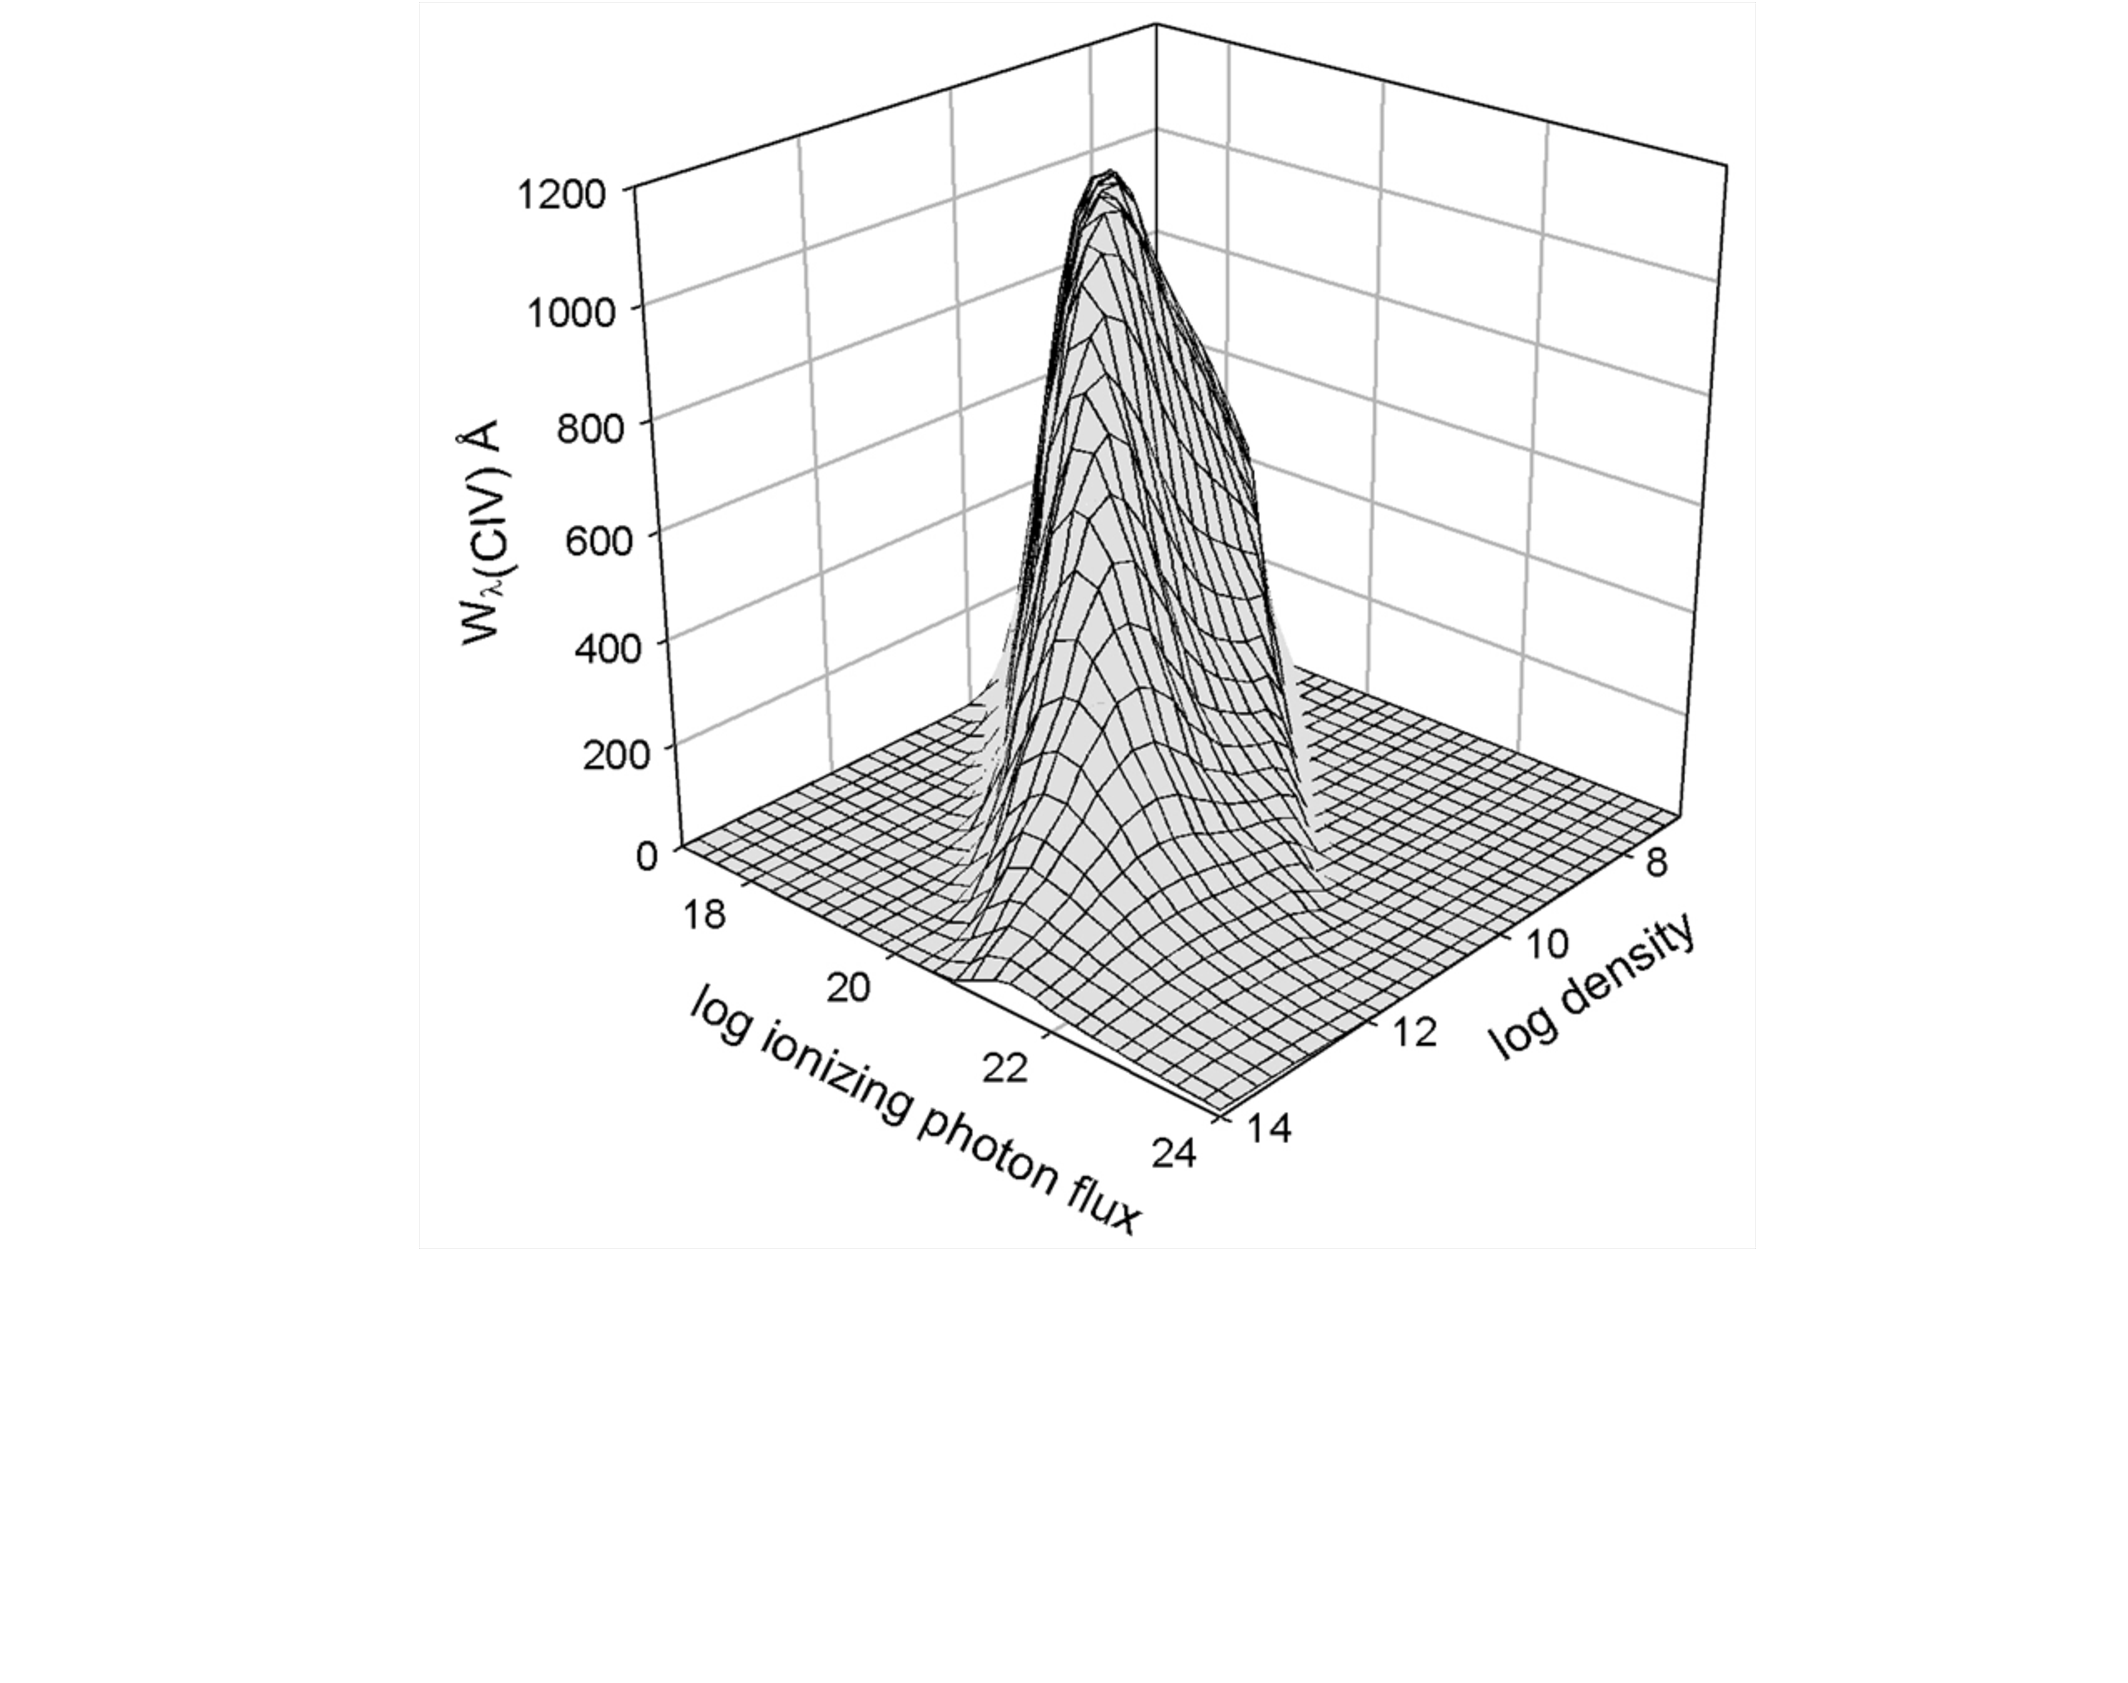
\includegraphics[scale=0.8]{CIV_EW}
\caption[C~IV equivalent width]{\label{fig:CIV_EW}The results of a large grid of quasar emission-line cloud
calculations are shown.  The $x$-$y$ plane shows the logs of the hydrogen density
(cm$^{3)}$ and flux of ionizing photons (cm$^{-2}$ s$^{-1}$).  The $z$ axis is the predicted
line equivalent width.}
\end{figure}

Much of this can be done without writing a program,
by using the \cdCommand{grid} command.
This command was introduced by Ryan Porter in C07.02, and makes
it possible to create large grids of models like those shown in
Figure \ref{fig:CIV_EW} with commands.
The \cdCommand{grid} command is described in Part 1 of this document.
There are several \cdCommand{save} output commands that are designed to save information
from grid calculations.

\begin{shaded}
\subsection{\experimental Host languages}

\Cloudy\ is written in C++, and it assumed for most of this section
that \Cloudy\ will be called from an external C or C++ program.

However, there is experimental support for a number of other
languages.

You can call a C++ program like \Cloudy\ from a Fortran program by
using the \cdTerm{cfortran.h} header file described at
\href{http://www-zeus.desy.de/~burow/cfortran/}{\tt
http://www-zeus.desy.de/$\sim{}$burow/cfortran/}.  I have never tried
this.  Good luck.

In the subdirectory \verb|sys_gcc_shared|, an additional set of
Makefile targets are set up to use the subroutine API described below
for Perl and Python scripts, using the SWIG interface generator.  In
this directory, there is also an experimental direct interface to the
Lua scripting language.
\end{shaded}

\subsection{Creating a new main program}

In C++ there must be exactly one main program
and it must be called \cdRoutine{main}.
This routine is within the file \cdFilename{maincl.cpp} in the source downloaded from
the web.
You need to replace the existing \Cloudy\ main program with one
that you write.
The file \cdFilename{maincl.cpp} that is included in the distribution
must be deleted so that the program you write will be loaded instead.
The
remaining routines are then compiled with a command like the following:
\begin{verbatim}
g++ -O3 -c *.cpp
\end{verbatim}
which will create a large number of object files.  The new main
program will then need to be linked with these object files with a
command something like
\begin{verbatim}
g++ -O3 -o mycloudy.exe newmain.cpp *.o -lm
\end{verbatim}

Alternatively, if you are using the Makefile build process and have
already built \Cloudy, you can use the library file \verb|libcloudy.a|
which contains all the object files with the command
\begin{verbatim}
g++ -O3 -o mycloudy.exe newmain.cpp -L. -lcloudy -lm
\end{verbatim}

The following subsections outline how to write code for this new main program.

\subsection{The cddefines.h and cddrive.h header files}

The file \cdFilename{cddrive.h} contains definitions of all public routines, the
routines that a user would call to drive \Cloudy.
That file is the definitive
reference for the material contained in this section and is more up to date
than this document.
Comments within that file explain all routines and
their parameters.

The header \cdFilename{cddefines.h} should come before \cdFilename{cddrive.h} since it includes
many definitions and includes the standard C++ header files that are needed
to drive the code.
The first two header files in the new main routine should
be the following:
\begin{verbatim}
#include "cddefines.h"
#include "cddrive.h"
\end{verbatim}

\subsection{The template for main programs }

C++ exceptions are used by \Cloudy.
The main program must catch these
exceptions.
If it does not then the code will crash with an unhandled
exception and output files will not be complete.
This requires that the
main program start with a C++ ``try'' block and that exception handlers
be included within the main program.
The adventurous user may enjoy creating
their own try block/exception handlers.

A sample template, in the file \cdFilename{template.cpp},
includes the needed code and can be
used to create your own programs.
It is included in the \cdFilename{programs} directory
below the \cdFilename{tsuite} directory in the program download.
That version includes
a simple call to run the code's smoke test.
You would replace the existing
code with your own.

\subsection{A note on return conditions}

Some of the routines return a value to indicate success or failure.
I try to follow the C and Unix conventions to indicate success with zero
(or \cdVariable{false}) and trouble with a non-zero return (or \cdVariable{true}).
This rule is not always followed (it
is not followed by the important routine \cdRoutine{cdLine}),
however, and \cdFilename{cddrive.h}
should be consulted to make sure the return conditions are understood.

\section{Initializing the code}

Many variables must be initialized at the beginning of the calculation.
Calling routine \cdRoutine{cdInit} does this.
\begin{verbatim}
cdInit();
\end{verbatim}
Routine \cdRoutine{cdInit} must be called every time
a new calculation is to be
performed, \emph{before} calling any of the following subroutines,
but after the
results of any previous calculations have been read.
(The results of any
previous calculations are lost when \cdRoutine{cdInit} is called.)

\section{Handling input and output}

\subsection{cdTalk---produce output?}

\Cloudy\ normally speaks what's on its mind.
This would generate too much
output in a large grid.
It does have a quiet mode in which nothing at all
is printed.
This quiet mode is set by the logical argument to subroutine
\cdRoutine{cdTalk}.
\begin{verbatim}
#include "cddefines.h"
#include "cddrive.h"
cdInit();
/*set no output at all*/
cdTalk( false )
/*have the code produce the normal printout*/
cdTalk( true )
\end{verbatim}

The default is for \Cloudy\ to produce output.
\cdRoutine{cdTalk} does not have to
be called if this is what you want.
It needs to be called with the logical
variable \cdRoutine{false} if the quiet mode is desired.

\subsection{cdOutput---sending output to a file}

\Cloudy\ normally writes its standard output on the system's
\cdFilename{stdout}. This can be changed to another file by calling the
routine \cdRoutine{cdOutput}, which has two arguments. The first is the name
of the file, and the second the mode with which the file should be opened
(this is identical to the second parameter of the fopen() routine). Both
parameters have default values. The default mode for opening the file is
``w'', while the default filename is the empty string. Supplying an empty
string as the file name means that the output will be directed back to
\cdFilename{stdout} again. The output file will be automatically closed on
exit of the program. If you call \cdRoutine{cdOutput} multiple times with
different file names, the file from the previous call will also be closed
automatically.
\begin{verbatim}
#include "cddefines.h"
#include "cddrive.h"

/* open the file output.txt for writing with mode "w" */
/* this will overwrite an existing file */
cdOutput("output.txt");

/* if you want to append to a file, use this instead */
cdOutput("output.txt","a");

/* this will close output.txt and open output2.txt with mode "w" */
cdOutput("output2.txt");

/* if you now want to redirect to stdout again, use this */
/* this will close output2.txt */
cdOutput();
\end{verbatim}

\subsection{cdInput---reading input from a file}

\Cloudy\ normally reads input from the system's \cdFilename{stdin}. This can
be changed to another file by calling the routine \cdRoutine{cdInput}, which
works the same way as the \cdRoutine{cdOutput} command described above with
the following two exceptions: the default open mode is ``r'', and supplying
an empty string as the file name redirects input back to \cdFilename{stdin}.

\subsection{cdRead---entering Commands}

Command lines are entered by successive calls to routine \cdRoutine{cdRead}.  The
argument of \cdRoutine{cdRead} is a null-terminated string containing valid commands.
These commands must obey all the rules outlined in Part~I.

In the examples below some commands are directly entered as strings (this
works when the string is a constant) while other strings are created by
writing variables through \cdRoutine{sprintf} (a standard C io function).  This is
necessary when the value of a variable needs to be placed into a string.
\begin{verbatim}
   char chLine[200];/* this string will hold the command lines we will generate*/

  /* this example sends the string straight to cdRead */
  nleft = cdRead("title a series of constant pressure models" );

  /* write variable to a string then sends the string to cdRead */
  hden = 5.4;
  sprintf( chLine , "hden %5.2f ", hden );
  nleft = cdRead(chLine );

  /* this example sends a string that contains double quotes,
  * and so must "escape" them with doubled backslashes */
  nleft = cdRead("save overview \"test.ovr\" " );

  sprintf( chLine , "coronal %5.2f ", temp );
  nleft = cdRead(chLine );

  nleft = cdRead("stop zone 1 " );
\end{verbatim}

\cdRoutine{cdRead} returns the number of commands that can still be entered before
exceeding the size of the storage arrays.
The return value was ignored
in the examples above.
So this routine is an exception to the general rule
that a zero return condition indicates success---here it indicates a
problem---no further commands can be entered.

It is not now possible to read in more than \NKRD\ command lines because
of limits to the size of the character arrays used to store them.  This
limit is stored as the variable \cdVariable{NKRD}.
If more than \NKRD\ lines are read
in by calling \cdRoutine{cdRead} then \cdRoutine{cdRead} will stop after explaining why.
It will
be necessary to increase \cdVariable{NKRD} if more than \NKRD\ command lines are needed.

\section{Executing the code}

\subsection{cdDrive---calling the Code}

The calculation is performed when routine \cdRoutine{cdDrive} is called.
\cdRoutine{cdDrive}
returns a bool indicating whether the calculation aborted.
The value
\cdVariable{false} indicates a successful calculation.
The following shows an example of
its use.
\begin{verbatim}
if( cdDrive() )
{
    printf("problems!\n");
    cdEXIT(EXIT_FAILURE);
}
\end{verbatim}

If problems occurred and the results cannot be trusted then the return
value is \cdVariable{true}.  This will only be set if the calculation suffered a
complete meltdown.  Routine \cdRoutine{cdNwcns} can be called to
find out about any problems.

\subsection{cdNoExec---checking without Computing}

If routine \cdRoutine{cdNoExec} is called after \cdRoutine{cdInit}
but before \cdRoutine{cdDrive} then only
the initial parts of a calculation will be performed when routine
\cdRoutine{cdDrive}
is called.
\begin{verbatim}
cdInit();

/*read in commands */
cdRead( . . .);

/*tell it not to execute */
cdNoExec();

/*call the code */
if( cdDrive() )
    cdEXIT(EXIT_FAILURE);
\end{verbatim}

When \cdRoutine{cdDrive} is called after \cdRoutine{cdNoExec} the code will generate the incident
continuum, set the initial density, and derive the chemical composition.
It will then stop just before the initial search for the physical conditions
in the first zone.  All of the initial printout, summarizing properties
of the composition and continuum, will be generated.  This provides a quick
way to check that a large grid of models will be specified correctly without
actually fully computing the grid.

\section{Ending the code}

The code must end by calling \cdRoutine{cdEXIT}.
This routine will close any open
output files and do other needed jobs before exiting.
The full output may
not be produced if this routine is not called.
Routine \cdRoutine{cdEXIT} takes a single
parameter, \cdRoutine{EXIT\_SUCCESS} or \cdRoutine{EXIT\_FAILURE},
standard macros that indicate how
the program ended.

The routine \cdRoutine{cdEXIT} is a pair with \cdRoutine{DEBUG\_ENTRY}.
Any routine that calls
\cdRoutine{cdEXIT} must also have a call to \cdRoutine{DEBUG\_ENTRY} statement at the start.  The
routine \cdRoutine{DEBUG\_ENTRY} has a single parameter, a string giving the name of
the routine (which should be ``main()'') in the case of the main program.

\section{Checking Predictions}

This section describes a series of routines that allow predicted
quantities to be obtained after the calculation is complete.

\subsection{cdB21cm---mean magnetic field}

The return value is the mean magnetic field weighted by
$n(\mathrm{H}^0) dr/T_{spin}$.
This is related to the field measured with 21 cm Zeeman
observations.
A tangled magnetic field is assumed.
A magnetic field is
not included by default but can be added with the
\cdCommand{magnetic field} command, described in Part 1 of this document.

\subsection{cdColm---the computed column densities }
\label{sec:SubroutineCdColm}

The predicted column densities of some species can be obtained by
calling routine \cdRoutine{cdColm}:
\begin{verbatim}
/* want N(C+2) */
if(cdColm("carb", 3 , &colum))
{
    printf(" could not find C+2\n");
}
else
{
    printf("The predicted C+2 column density is %e\n", column );
}
\end{verbatim}
The routine returns zero if it found the species, and 1 if it could not.
It returns the predicted column density [\pscm] as the third argument.  The
first argument \cdVariable{chLabel} is a four-character string that must agree with the
first four characters (upper or lower case) of the name used to indicate
the element in the printout.
The second (integer) variable \cdVariable{ion} is the
spectroscopic designation of the level of ionization, i.e., 1 indicates
the atom C$^0$, 3 indicates C$^{+2}$, etc.

The ion stage of 0 indicates a special case, a molecule or an excited
level of an atom or ion.  The label determines the species in this case.
Table \ref{tab:cdColm_labels} gives the levels and molecules that
are recognized.  Many of the
molecules have fewer than four characters.
The label must still contain
four characters and spaces are used to fill out the four.

\begin{table}
\centering
\caption{Special cases  cdColm Column Densities}
\label{tab:cdColm_labels}
\begin{tabular}{lcc}
\hline
\multicolumn{2}{c}{Excited
states}& molecules\\
\hline
Label& Level& Label\\
\hline
He1*& He$^0$ 2$^3$S& H2\\
CII*& C$^+ J = 3/2$& H-\\
C11*& C$^0
J = 0$& H2+\\
C12*& C$^0 J = 1$& H3+\\
C13*& C$^0 J = 2$& H2g\\
C30*& C$^{2+} J = 0$& H2*\\
C31*& C$^{2+}
J = 1$& HeH+\\
C32*& C$^{2+} J = 2$& CO\\
O11*& O$^0 J = 2$& OH\\
O12*& O$^0 J = 1$& H2O\\
O13*& O$^0
J = 0$& O2\\
Si2*& Si$^+ J=3/2$& SiO\\
&&H-\\
&&C2\\
&&C3\\
&&CN\\
&&CH\\
&&CH$^+$\\
H2vJ& \htwo\ any
$v,J$& H2\\
\hline
\end{tabular}
\end{table}

A large and complex model of the \htwo\ molecule is computed when the
\cdCommand{atom H2} command is included.
It is possible to obtain column densities in any
$v,J$ level of \htwo\ by calling routine \cdTerm{cdH2\_colden}.

\subsection{cdCooling\_last---last zone's cooling}

The return value is the total cooling rate (erg cm$^{-3}$ s$^{-1}$)
for the last computed zone.

\subsection{cdDepth\_depth---the depth structure of the cloud}

This routine returns a vector giving the zone depths (in cm) of the
previous iteration.
The code uses adaptive logic to control the radial
zoning of the model.
Neither the number of depth points nor their structure
is known in advance.
This routine is called with a double precision vector
with enough space to hold the structure.
The number of depth points is
determined by calling \cdRoutine{cdnZone} and space must be allocated by the calling
routine.
Each element of the vector is the depth from the illuminated face
to the center of zone~$n$.

\subsection{cdEDEN\_last---electron density of last zone}

This returns the electron density ($\pcc$) of the last zone.

\subsection{cdEmis---emissivity of lines}

\cdRoutine{cdEmis} has the same arguments as \cdRoutine{cdLine}
but returns the
local emissivity (erg cm$^{-3}$ s$^{-1}$ for unit filling factor) of the line for
the last computed zone.
The return value is the index of the line within
the line stack if it was found, and the negative of the number of lines
in the stack if the line could not be found.

\subsection{cdGetLineList---sets of emission lines}

The routine \cdRoutine{cdGetLineList} provides a way
to automatically access a list of emission lines.

First enter a list of emission lines into a file.
One emission line
occurs on each line of the file.  It starts with a line label like
``H~~1'' followed by the wavelength of the line.
A set of such files is included
in the data directory of the distribution files.  They have names
\cdFilename{LineList*.dat}.  You can use these as examples to create your own files.

The first argument to routine \cdRoutine{cdGetLineList} is the name of the file
containing the line list.  If a null string is passed (``'') then
\cdFilename{LineList\_BLR.dat} is used.  The code will first try to open the file in the
current directory, and if is not present, will try on the path.

\cdRoutine{cdInit} must be called before \cdRoutine{cdGetLineList} is called.
Next \cdRoutine{cdGetLineList}
is called, and finally, the actual grid of calculations begins.  The
predicted intensities of a set of lines are then extracted by calling
\cdRoutine{cdLine}.

The second and third parameters are a pair of vectors that are defined
by the calling program.
When the routine \cdRoutine{cdGetLineList} is called it uses these
vectors to store the labels and wavelengths.
Space for the lines is allocated by \cdRoutine{cdGetLineList} after it determines how
many lines are in the file.  These string and float vectors will then contain
the label and wavelength used to identify the lines.  The function returns
the number of lines in the list.  If problems occurred then $-1$ is returned.

The following shows an example of getting the lines from
\cdFilename{LineList\_NLR.dat},
executing the code, and then obtaining the predicted intensities of all
lines listed in \cdFilename{LineList\_NLR.dat}
by calling \cdRoutine{cdLine}.
\begin{verbatim}
/* define variables */
exit_type exit_status = EXIT_SUCCESS;
vector<char*> chLabel;
vector<float> wl;
/* initialize the code */
cdInit();
/* get list of lines from a line list included in the distribution */
if( (nLines=cdGetLineList("LineList_NLR.dat",chLabel,wl)) < 0 )
{
    /* this is the error exit - could not obtain the lines */
    cdEXIT(EXIT_FAILURE);
}
- - - - - - missing code
/* now do the calculation */
cdInit();
/* missing commands here, then call the code */
- - - - - - missing code
if( cdDrive() )
    exit_status = EXIT_FAILURE;
- - - - - - missing commands go here
/* now print the predicted emission line intensities */
for( long n=0; n < nLines; ++n )
{
    if( cdLine( chLabel[n], wl[n], &relative, &absolute ) < 0 )
    {
        fprintf(stderr,"did not find %4s%5li\n",chLabel[n],wl[n]);
    }
    print("%.3e\n", relative);
}
/* free the memory that was allocated in cdGetLineList */
for( size_t i=0; i < chLabel.size(); ++i )
    delete[] chLabel[i];
chLabel.clear();
cdEXIT(exit_status);
\end{verbatim}

\subsection{cdH2\_colden---state-specific column densities of \htwo}

This returns the column density of any level in the X ground
electronic state of \htwo.
This command only works when the large \htwo\ molecule
is included with the \cdCommand{atom H2} command.
It has two integer arguments, the
vibration and rotation quantum numbers of a level in X.
If both are zero
or greater the routine returns the column density in that level.
If the
vibration quantum number is negative then a summed column density is turned.
If $v<0$ and $J=0$ it returns the total \htwo\ column density, if $J=1$ it returns
the ortho column density, and if $J=2$ the para column density.
If the indices
do not make sense the routine prints a message and returns~$-1$.

Here are some examples:
\begin{verbatim}
/* total H2 column density */
total = cdH2_colden( -1 , 0 );
/* ortho column density */
ortho = cdH2_colden( -1 , 1 );
/* para column density */
para = cdH2_colden( -1 , 2 );
/* column density in 0, 0 */
total00 = cdH2_colden( 0 , 0 );
\end{verbatim}

\subsection{cdH2\_Line---an \htwo\ emission line intensity}

More than half a million \htwo\ lines are predicted and there will be
instances where two \htwo\ lines have nearly the same wavelength.  Identification
of a particular transition within the list of lines can be ambiguous.  This
command finds the intensity and luminosity of a transition by specifying
its upper and lower $n, v, J$ levels.
The first six arguments give the $n,
v, J$ indices of the upper and lower levels in that order.
The last two
variables are double pointers that return the intensity and luminosity of
the transition.
The function returns 1 if it finds the line and 0 if it
did not.
(This behavior follows that of \cdRoutine{cdLine} rather than the standard
C++ conventions on function return values.)
Currently this only works
for the ground electronic state.

Here is an example:
\begin{verbatim}
double xInten , xLumin;
/* the 1-0 S(1) at 2.121 microns */
if( cdH2_Lines( 0,1,3 , 0,0,1 , &xInten , &xLumin ) == 0 )
{
    printf("could not find line.\n");
}
\end{verbatim}

\subsection{cdHeating\_last---last zone's heating}

The total heating rate (erg cm$^{-3}$ s$^{-1}$)
for the last computed zone is returned.

\subsection{cdIonFrac---the computed ionization fractions}

The predicted ionization fractions,\footnote{Before version 96 the ionization fractions only included atoms and
ions.  They now also include molecules.  The sum of the atomic and ionic
fractions will not add up to unity if a significant fraction of the element
is in molecules.} averaged over radius, area, or volume,
can be accessed by calling the subroutine \cdRoutine{cdIonFrac}.
The average over radius is defined as
\begin{equation}
\left\langle {\frac{{n\left( {{S^{ + n}}} \right)}}{{n\left( {{S_{gas}}}
\right)}}} \right\rangle  = \frac{{\int_{}^{} {\,n({S^{ + n}})\;f(l)\,d{\kern
1pt} l} }}{{\int_{}^{} {n({S_{gas}})\;f(l)\,d{\kern 1pt} l} }}
\end{equation}
where $n(S_{gas})$ is the total gas phase density of the element.
The average
over area is defined as
\begin{equation}
\left\langle {\frac{{n\left( {{S^{ + n}}} \right)}}{{n\left( {{S_{gas}}}
\right)}}} \right\rangle  = \frac{{\int_{}^{} {n({S^{ + n}})\;f(r)\,r\,dr}
}}{{\int_{}^{} {n({S_{gas}})\;f(r)\,r\,dr} }}.
\end{equation}
The average
over volume  is defined as
\begin{equation}
\left\langle {\frac{{n\left( {{S^{ + n}}} \right)}}{{n\left( {{S_{gas}}}
\right)}}} \right\rangle  = \frac{{\int_{}^{} {n({S^{ + n}})\;f(r)\,r^2\,dr}
}}{{\int_{}^{} {n({S_{gas}})\;f(r)\,r^2\,dr} }}.
\end{equation}

Two sample calls to the routine follow:
\begin{verbatim}
/* false below means to not include electrons in the mean */
if( cdIonFrac("carb", 2, &frac, "radius", false) )
{
    cdEXIT(EXIT_FAILURE);
}
printf("The predicted ionization fraction over radius is %g\n", frac);
/* true below means to include electrons in the mean */
if( cdIonFrac("carb", 2, &frac, "radius", true) )
{
    cdEXIT(EXIT_FAILURE);
}
printf("Ionization fraction wrt radius end elec den is %g\n", frac);
\end{verbatim}
The first argument is a four-character identifier that must agree with the
first four characters (upper or lower case) used to indicate the element
in the printout.  The second integer argument is the spectroscopic
designation of the level of ionization, i.e., 1 indicates C$^0$,
3 indicates the second ion C$^{+2}$, etc.
The third argument returns the predicted ionization
fraction $S^{+n}/S_{gas}$.
The 4th argument is a six-character variable (plus end
of string sentinel) which must be either ``\cdVariable{radius}'', ``\cdVariable{area}'', or
``\cdVariable{volume}'' (either
upper or lower case).
This string determines whether the ionization fraction
returned is weighted with respect to radius, area, or volume.
These would be appropriate to compare to pencil beam observations,
integrated long slit observations, or observations of the whole nebula, respectively.
The last argument
determines whether (\cdVariable{true}) or not (\cdVariable{false})
the ionization fraction is also
weighted with respect to the electron density.
The function returns zero
if the ion was found and non-zero if an error occurred.

An ionization stage of zero will request the fraction of an element
within a molecule.
If the element name is ``H2~~`` (the letters H2 followed
by two spaces) then the fraction of hydrogen in \htwo,
$2n$(H$_2)/n(H_{tot})$, will
be returned.  Currently only \htwo\ is implemented.

\subsection{cdLine---emission-line intensities }

This finds the intensity or luminosity of any line.  The label and
wavelength of the line are specified and the routine returns the relative
intensity and the log of the absolute intensity or luminosity.
The following is an example.
\begin{verbatim}
#include "cddefines.h"
#include "cddrive.h"
double relint , absint;
long nType=0;

if( cdLine( "totl" , 4861 , &relint , &absint , nType ) < 0 )
    printf("did not find this line\n");
\end{verbatim}

The first argument in the call is the line label, the four-character
null-terminated string (upper or lower case) used by the code to identify
the line in the main emission-line printout.  The second variable gives
the wavelength of the line in Angstroms.  Both of these must exactly match
the label and wavelength used by \Cloudy\ to identify the line
(see the chapter \cdSectionTitle{Lines} for a full description).
The third variable (\cdVariable{relint} in the above
example) is a double-precision pointer to the relative intensity of the
line (relative to the normalization line, usually H$\beta$,
and reset with the
\cdCommand{normalize} command).
The log of the intensity (erg
cm$^{-2}$~s$^{-1}$) or luminosity
(erg s$^{-1}$) of the line is returned as the fourth double-precision pointer
(\cdVariable{absint} in the above example).
If the intensity of the line is zero or
the line was not found then this variable will be set to $-37$.

The last (optional) parameter indicates which type of line prediction to return.
The integer types are
 0 intrinsic, 
 1 emergent, 
 2 intrinsic cumulative, 
 3 emergent cumulative
 intensities.

The intensities returned by when the last parameter is missing
or it is zero are those printed with the
heading \emph{Intrinsic Intensities}.
This does not include the effects of possible
reflection off a background molecular cloud or of absorption from outside
the emission-line region.
If the last parameter is 1 then emergent
intensities are reported.
The values 2 and 3 are the equivalent quantities for the cumulative
intensities in a time dependent model.

If \cdRoutine{cdLine} finds the line it returns the index of the line within the
stack of emission lines.
So a positive return value indicates success.
It returns the negative of the total number of lines in the stack if the
line is not found.  This may occur if the line wavelength or label was
mistyped.  This is an exception to the C++ function return convention in
which a normal return is zero and an abnormal return is non-zero.  A positive
value indicates a successful return.

There is a special version, \cdRoutine{cdLine\_ip},  which takes the line index as
the first argument and return the relative and absolute intensities as the
second and their quantities.  The line index is not a constant for a given
version of the code.  It depends on the number of elements that are included,
the sizes of the iso-sequence model atoms, and whether other models like
\htwo\ are included.

\subsection{cdnZone---how many zones in the last iteration?}

The routine returns the number of zones in the previous iteration.

\subsection{cdPressure\_depth---pressure structure of the last iteration }

The pressure as a function of depth, for the last iteration, is obtained
by calling routine \cdRoutine{cdPressure\_depth}.  This routine has three arguments,
pointers to vectors giving the total pressure, the gas pressure, and the
line radiation pressure.  All are double precision vectors and the calling
routine must have allocated space for these before calling the routine.
The total number of elements needed for each vector is the number of zones
in the last iteration and is obtained by calling routine \cdRoutine{cdnZone}.

\subsection{cdPressure\_last---pressure of the last zone }

The pressure for the last zone is obtained by calling routine
\cdRoutine{cdPresure\_last}.
This routine has three arguments, pointers to the total
pressure, the gas pressure, and the line radiation pressure.
All are double
precision variables.
The total pressure includes all contributors to the
pressure and may include magnetic, radiation, and turbulent pressure in
addition to thermal pressure.

\subsection{cdSPEC---get predicted spectrum}

This routine provides an interface between \Cloudy\ and Keith Arnaud's
X-Ray spectral analysis program \cdRoutine{XSPEC}.
Depending on which option is used,
it will return the incident continuum, the attenuated incident continuum,
the reflected continuum, the diffuse continuous continuum, outward direction
diffuse continuous emission, reflected lines, or outward lines.
All are
$4\pi \nu J_\nu$ [erg cm$^{-2}$ s$^{-1}$] and assume full coverage of the continuum source.
Details are given in \cdFilename{cddrive.h}.

This is no longer being developed and will soon be removed.
Use the
\cdCommand{save FITS} command, described in Part 1, instead.

\subsection{cdTemp---the computed mean temperature}
\label{sec:SubroutineCdTemp}

Routine \cdRoutine{cdTemp} returns the mean electron temperature weighted with respect
to some species.
The first parameter is a four character null-terminated
string giving the first four letters (upper or lower case) of the name of
an element as spelled by the code.
The second parameter is the ionization
stage, with 1 for the atom, 2 the first ion, etc.
The third parameter will
be the computed mean temperature.
The last parameter is a six-character
null-terminated string, either ``radius'', ``area'', or ``volume'', that says whether
the temperature should be weighted with respect to radius, area, or volume.
These would be appropriate to compare to pencil beam observations,
integrated long slit observations, or observations of the whole nebula, respectively.
The mean temperature weighted by ion $+n$ of element $S$ over radius
is defined as
\begin{equation}
\left\langle {T\left( {{S^{ + n}}} \right)} \right\rangle  =
\frac{{\int_{}^{} {T\,n({S^{ + n}})\;f(l)\,d{\kern 1pt} l} }}{{\int_{}^{}
{n({S^{ + n}})\;f(l)\,d{\kern 1pt} l} }}\quad [\mathrm{K}],
\end{equation}
the average over area is
\begin{equation}
\left\langle {T\left( {{S^{ + n}}} \right)} \right\rangle  =
\frac{{\int_{}^{} {T\,n({S^{ + n}})\;f(r)\,r\,dr} }}{{\int_{}^{} {n({S^{ +
n}})\;f(r)\,r\,dr} }}
\quad [\mathrm{K}],
\end{equation}
and the average over volume  is
\begin{equation}
\left\langle {T\left( {{S^{ + n}}} \right)} \right\rangle  =
\frac{{\int_{}^{} {T\,n({S^{ + n}})\;f(r)\,r^2\,dr} }}{{\int_{}^{} {n({S^{ +
n}})\;f(r)\,r^2\,dr} }}
\quad [\mathrm{K}] .
\end{equation}
The routine returns 0 if it finds the species, and 1 if it could not find
the species.  The following is an example of a call:
\begin{verbatim}
if( cdTemp("carb", 2, &temp, "radius") )
{
    cdEXIT(EXIT_FAILURE);
}
printf("The mean C+2 temperature is %g\n", temp);
\end{verbatim}

An ionization stage of zero requests one of the following special
temperatures. All these can be weighted by radius, area, or volume.
\begin{description}
\item[21 cm-related temperatures:]  The routine will return one of three
temperatures related to 21 cm observations.
The label ``\cdTerm{21cm}'' will return
the mean of $n(\mathrm{H}^0)/T_{kin}$, the harmonic mean gas kinetic temperature weighted
with respect to the atomic hydrogen density.
The label ``\cdCommand{spin}'' will return the mean weighted by
$n(\mathrm{H}^0)/T_{spin}$, the harmonic mean of the 21 cm spin temperature weighted with
respect to the atomic hydrogen density.
Finally the label ``\cdCommand{opti}'' returns the
temperature derived from the ratio of L$\alpha $ to 21
cm optical depths (see AGN3 section 5.5).

\item[Molecular hydrogen:]  The label ``\cdCommand{H2\_\_}'' (notice that there were two spaces
after the 2) and an ionization stage of zero will return the mean temperature
weighted with respect to the \htwo\ density.

\item[Simple mean temperature:]  If the label consists of four spaces, as in
``~~~~``, and the ionization stage is zero, the routine will return the
mean temperature, but not weighted by any
species. If the label is ``\cdCommand{TeNe}'' then the routine will return
the mean temperature weighted by the electron density.
\end{description}

\subsection{cdTemp\_last---the temperature of the last zone}

The kinetic temperature of the last zone is obtained by calling the
function \cdRoutine{cdLastTemp}.
The function has no arguments and its return value
is the temperature.

\subsection{cdTimescales---several timescales.}

This routine has three arguments, pointers to doubles that return the
timescales [s] for several processes.
These are the thermal timescale,
the hydrogen recombination timescale, and the \htwo\ formation timescale.

\section{Other information}

\subsection{cdDate(cdString)}

The date when the current version of the code was released will be placed
as a null-terminated string.  The string is passed as an argument and the
calling program must have allocated enough room for the string.

\subsection{cdVersion(cdString)}

The code's version number will be placed as a null-terminated string
into the string passed as an argument.
The version number is a string rather
than a float since it can end with a letter of the alphabet.
The calling
program must allocate enough space for the string.

\subsection{double cdExecTime()}

This returns the time that has elapsed since the previous call
to \cdRoutine{cdInit}.

\section{Printing comments}

\Cloudy\ is designed to be autonomous and self aware.
It constantly
monitors itself to make sure that it is doing the physics correctly.  After
the calculation is complete, but before the emission lines are printed,
it generates a series of statements that indicate warnings, cautions,
comments, and surprises.
These should be examined to confirm that the
calculation is likely to be valid.
A series of routines allows the driving
code to determine whether these comments were generated, what type they
were, and to print then into an arbitrary open file.

\subsection{Were comments generated?}

Routine \cdRoutine{cdNwcns} will return the number of warnings, cautions, surprises,
notes, and temperature and pressure failures:
\begin{verbatim}
 cdNwcns( &lgAbort , &nw , &nc , &nn , &ns , &nte , &npe , &nione, &neden )
\end{verbatim}
where the first variable is a \cdVariable{bool} flag indicating whether the calculation
aborted, \cdVariable{nw} is the number of warnings generated (if this number is non-zero,
then the calculation has serious problems), \cdVariable{nc} is the number of cautions
generated (these are less severe than warnings, but are still a cause of
concern), and \cdVariable{nn} and \cdVariable{ns} are the number of notes and surprises.
The next
two arguments are the number of temperature and pressure failures.
The
last two are the number of ionization and electron density failures.  There
should not be any failures in a successful calculation.

If either of the first two variables are non-zero then the code ran into
serious problems.  An abort is far more serious than a warning since it
indicates catastrophic failure.  I would appreciate learning about these.
Please post details on the code's discussion board.

\subsection{Printing the comments.}

A series of comments normally appear after the last zone.  These may
be printed into any file by calling the series of subroutines described
here.  In all cases the routines take as an argument a file handle which
must point to a file that has already been opened for writing.
\begin{verbatim}
/* output the comments into a file
 * first define the file handle, then open the file for writing */
FILE *ioOUT;
if( (IoOUT = fopen( "comments.txt", "w") ) == NULL )
{
    printf("error creating comments.txt file\n");
    cdEXIT(EXIT_FAILURE);
}
--- missing code to do calculation  ---
/*print the reason the calculation stopped, and geometry*/
cdReasonGeo(ioOUT);
/*print the warnings*/
cdWarnings(ioOUT);
/*next print the cautions*/
cdCautions(ioOUT);
/*now print any surprising results*/
cdSurprises(ioOUT);
/*now print the notes*/
cdNotes(ioOUT);
fclose(ioOUT);
\end{verbatim}

\begin{description}
\item[cdReasonGeo(FILE *io)]  It is very important to understand why the calculation stopped.
The first two lines after the last zone results give the reason
the calculation stopped and the type of geometry.
This information will
be printed into the file whose handle is the argument.

\item[cdWarnings(FILE *io)]  All warnings (denoted by ``W-'') will be printed.

\item[cdCautions(FILE *io)]  All cautions (denoted by a ``C-'') will be printed.

\item[cdSurprises(FILE *io)]  All surprises (denoted by a ``!'') are printed.

\item[cdNotes(FILE *io)]  The notes concerning the calculation will be printed.
\end{description}

\subsection{cdErrors(FILE *io)---printing a summary of any problems}

Routine \cdRoutine{cdErrors(FILE *io)} will generate a summary
of any problems that happened during a calculation.
The argument is a pointer to the output
file where the summary will be placed.
The calling program must have already
opened the file for writing.
If problems occurred in the calculation, such
as temperature or pressure failures, warnings, or cautions,
will be printed
along with the calculation's title.

\subsection{cdPrintCommands(FILE *io)---print the command stack}

The entire series of input commands will be written into the file.  The
single argument is a file handle that points to a previously opened file.
The commands are preceded and followed by lines that begin with
``c~=====''
to easily identify their start and end.

\subsection{setbuf or the no buffering command}

Programs produce output by writing into a buffer.
They only place
information on the disk once the buffer is full.
If a C++ program
crashes before this buffer is ``flushed'' the information within the buffer
will be lost.
This poses a problem if the printout generated just before
the crash is needed for debugging.
The C++ io library provides a routine,
\cdRoutine{setbuf}, that can turn file buffering off.
The following sequence would
open a file and turn buffering off:
\begin{verbatim}
ioDATA = open_data("test.out","w",AS_LOCAL_ONLY);
/* turn off buffering so we see results as then happen */
setbuf( ioDATA , NULL );
\end{verbatim}

Note that the call to \cdRoutine{setbuf} {\em must} come immediately after the
call to \cdRoutine{open\_data} before any output is written.
The \cdCommand{no buffering} command, described in Part 1 of this document, will do the same thing.
Note that turning off buffering will make the code run far more slowly.

\section{Example Call as a Subroutine}

The file \cdFilename{template.cpp} shown below contains a skeleton program
showing how you can call Cloudy as a subroutine. You can find the program in
the directory \cdFilename{tsuite/programs}. Use this as a starting point to
write your own program. The area where you can insert your own code is clearly
indicated in the template.
{ \setverbatimfontsize{\tiny}
\verbatimtabinput{../../../tsuite/programs/template.cpp}
}

\section{Computing Grids of Calculations}

Today I usually use the code to compute results, extract information, and save
desired quantities. The following example illustrates producing a series of
models with increasing gas temperature and density. The program calculates the
line strength of various diagnostic [\oiii] lines normalized to [\oiii]
$\lambda $5007 and writes these to a file. This example is the program
\cdFilename{vary\_nete.cpp}, which you can find in the directory
\cdFilename{tsuite/programs/vary\_nete}.

This example only saves results for a few lines. Often a large number of
lines are needed. A call to \cdRoutine{cdLineList} provides an easy way to
obtain large numbers of lines whose labels are stored in a file.
{ \setverbatimfontsize{\tiny}
\verbatimtabinput{../../../tsuite/programs/vary_nete/vary_nete.cpp}
}
          %proof 1
\chapter{THE EMISSION LINES}
% !TEX root = hazy2.tex
\label{sec:EmissionLines}

\section{Overview}

The following sections outline the emission lines predicted by \Cloudy.
Before version 90 of the code all lines were listed in the sub-section
immediately following this section.  The code is being modified to bring
all lines into a common line class, as the code moves to C++ and objects.
This chapter will remain incomplete until this work is finished.

\section{The main emission-line printout }

The main emission line printout was briefly described
in the Chapter \cdSectionTitle{OUTPUT}.
This section
goes into more detail.

\cdCommand{Output organization}.  The printed list is sorted into four large groups
of columns, with each large column sub-divided into four smaller sub-columns.
The first sub-column is either the spectroscopic designation of the ion
producing the line or an indication of how the line is formed.  The second
sub-column is the line wavelength, with a 0 to indicate a continuum.  The
third sub-column is the log of the power in the line, in the units given
in the header (erg s$^{-1}$ into either $4\pi$ sr or cm$^{-2}$).  The last sub-column is
the intensity of the line relative to the reference line,
usually H$\beta$ , unless
this is reset with the \cdCommand{normalize} command.

These lines can be printed as a single large column, and can be sorted
by wavelength or intensity.  These options are controlled by the
\cdCommand{print line}
command described in Part I of this document.

\subsection{Intrinsic and emergent line intensities}

The computed emission-line spectrum is divided into two groups.  The
first group of lines, called ``Intrinsic line intensities'', gives the
intrinsic intensity of the lines, and does not include the reddening effects
of internal grains due to the photon's passage out of the nebula.  The second
group includes the effects of grain scattering and absorption and has the
header ``Emergent Line Intensities''.  The intensities are the total
intensities observed from the illuminated face, including both absorption
and scattering by grains.

\subsection{Line identification}

\cdCommand{Line wavelengths}.  These are given in various units.
Numbers ending
in ``A'' are wavelengths in Angstroms (\AA ).
For instance, H$\beta$ is given by ``H~~1  4861A''.
Wavelengths in microns are indicated by ``m'', an example,
the strong [O~III] IR line, is ``O~~3 51.80m''.

The code follows the convention that wavelengths longward of 2000\AA\
are given in air and shorter wavelengths in vacuum.
Continua are usually
indicated by a wavelength of zero.

\subsection{Blocks of lines\dots}

Lines are organized by common origin with a comment, ending in a series
of periods ``\dots'', beginning the section.
As an example, the first
commented block of lines begins with ``general properties\dots''.
The
following subsections give overviews of the lines.

\subsection{General properties\dots}

This mainly summarizes heating and cooling agents for the model.
\begin{description}
\item[TOTL 4861 and TOTL 1216,] are the total intensities of H$\beta$
and L$\alpha $, as
predicted by the multi-level H atom.
These intensities are the results
of calculations that include all collisional, radiative, and optical
depth effects.

\item[Inci]  The total energy in the incident continuum.
This entry will not be included if the \cdCommand{aperture} command is in effect.

\item[TotH and TotC] give the total heating and cooling.  These will be nearly
equal in equilibrium.

\item[BFH1 and BFHx] are the heating due to photoionization of ground state
and excited state hydrogen respectively.

\item[He1i, 3He1], heating due to ground state He and the triplets.

\item[BFHe and TotM] are the heating due to helium and metal photoionization.

\item[Pair] heating due to pair production.

\item[ComH , ComC],  Compton heating, cooling.

\item[CT H    CT C] charge transfer heating and cooling.

\item[extH   extC]    ``extra'' heating or cooling added to model.

\item[e-e+  511]  The positron line.

\item[Expn], expansion, or adiabatic, cooling

\item[H FB], H radiative recombination cooling

\item[HFBc, HFBc], hydrogen net free-bound cooling and heating

\item[Iind], cooling due to induced recombination of hydrogen

\item[3He2], cooling due to induced recombination of fully ionized helium

\item[Cycn], cyclotron cooling
\end{description}

\subsection{Continua\dots}

These give intensities of various continua.  These are either the total
integrated continuum or the product $\nu F_\nu$ at certain energies.

\subsubsection{Continuum bands}
The file \cdFilename{continuum\_bands.ini} in the data directory
specifies a set of wavelength bands.
The code will integrate over these bands to find the
total radiated luminosity and enter this into the main emission-line stack.
Currently this is a simple sum of the energy emitted between the upper and
lower bounds of the band, and does not take into account the transmission function
of particular instruments.
The \cdFilename{continuum\_bands.ini} file can be edited to change 
the number of bands or their detailed properties.
Table \ref{tab:continuum_bands} lists the bands in the file at the
time of this writing.
The first and second columns give
the label and wavelength as they appear in the printout.
The last column
gives the wavelength range for the integration.
These entries will not be included if the \cdCommand{aperture} command is in effect.
Please consult the file to see its current contents
and feel free to add your own bands.

%copied from ini file 2012 July 20
% commented out code to print this is in cont_createpointers.cpp
% search for string *hazy table*
\begin{table}
\centering
\caption{\label{tab:continuum_bands}Default continuum bands}
\begin{tabular}{lll}
\hline
Label& Wavelength&Wavelength Range\\
\hline
 FIR  & 83.00m & 40.00m -- 500.0m\\ 
 TIR  &  1800m & 500.0m --  3100m\\ 
 NIRa & 2.850m &  7000A -- 40.00m\\ 
 NIRb & 3.000m & 10000A -- 5.000m\\ 
 MIRa & 15.00m & 5.000m -- 25.00m\\ 
 MIRb & 22.50m & 5.000m -- 40.00m\\ 
 NMIR & 21.75m &  7000A -- 40.00m\\ 
 TFIR & 611.2m & 122.5m --  1100m\\ 
 TALL & 10000A & 0.010A -- 10000m\\ 
 F12  & 12.00m & 8.500m -- 15.00m\\ 
 F25  & 25.00m & 19.00m -- 30.00m\\ 
 F60  & 60.00m & 40.00m -- 80.00m\\ 
 F100 & 100.0m & 83.00m -- 120.0m\\ 
 MIPS & 24.00m & 20.80m -- 26.10m\\ 
 MIPS & 70.00m & 61.00m -- 80.00m\\ 
 MIPS & 160.0m & 140.0m -- 174.0m\\ 
 IRAC & 3.600m & 3.160m -- 3.920m\\ 
 IRAC & 4.500m & 4.000m -- 5.020m\\ 
 IRAC & 5.800m & 5.000m -- 6.400m\\ 
 IRAC & 8.000m & 6.500m -- 9.300m\\ 
 SPR1 & 250.0m & 212.0m -- 288.0m\\ 
 SPR2 & 350.0m & 297.0m -- 405.0m\\ 
 SPR3 & 500.0m & 414.0m -- 600.0m\\ 
 PAC1 & 70.00m & 60.00m -- 82.00m\\ 
 PAC2 & 100.0m & 84.00m -- 122.0m\\ 
 PAC3 & 160.0m & 130.0m -- 198.0m\\ 
 PAH  & 3.300m & 3.250m -- 3.350m\\ 
 PAHC & 3.230m & 3.200m -- 3.250m\\ 
 PAHC & 3.370m & 3.350m -- 3.400m\\ 
 PAH  & 6.200m & 5.900m -- 6.400m\\ 
 PAHC & 5.650m & 5.400m -- 5.900m\\ 
 PAH  & 7.900m & 7.400m -- 8.400m\\ 
 PAHC & 6.900m & 6.400m -- 7.400m\\ 
 PAH  & 11.30m & 11.10m -- 11.50m\\ 
 PAHC & 10.90m & 10.70m -- 11.10m\\ 
 PAH  & 11.80m & 11.60m -- 12.30m\\ 
 PAHC & 12.65m & 12.30m -- 13.00m\\ 
 PAH  & 13.30m & 12.90m -- 13.70m\\ 
 PAHC & 14.10m & 13.70m -- 14.50m\\ 
 Bcon &  3640A & 911.6A --  3646A\\ 
 Pcon &  5000A &  3646A --  8204A\\ 
\hline
\end{tabular}
\end{table}

\subsubsection{Other continua}

\begin{description}
\item[Bac  3646]  residual flux at head of Balmer
continuum, $\nu F_\nu$. This entry will not be included if the \cdCommand{aperture}
command is in effect.

\item[cout 3646 cref 3646], outward, reflected continuum at peak of Balmer Jump.
These entries will not be included if the \cdCommand{aperture} command is in effect.

\item[thin 3646], residual flux at head of Balmer continuum, optically thin limit.
This entry will not be included if the \cdCommand{aperture} command is in effect.

\item[Inci 4860, Inci 1215], incident continua near \ha\ and \la.
These entries will not be included if the \cdCommand{aperture} command is in effect.

\item[Ba C    0], integrated Balmer continuum

\item[PA C    0], integrated Paschen continuum

\item[HeFF    0], He brems emission

\item[HeFB    0], He recombination cooling

\item[MeFB    0], heavy element recombination cooling

\item[MeFF    0], metal brems emission

\item[ToFF    0], total brems emission

\item[FF x], part of H brems, in x-ray beyond 0.5KeV

\item[eeff], electron - electron brems
\end{description}

\cdTerm{nFnu  122m},
\cdTerm{nInu  122m},
\cdTerm{InwT  122m},
\cdTerm{InwC  122m},
a large list of continua
at selected wavelengths will be printed if the
\cdCommand{print continuum}
command is entered.
These entries will not be included if the \cdCommand{aperture} command is in effect.
The first is the sum of various continua at the wavelength,
given as $\nu F_\nu$ (see the \cdCommand{print continuum} and \cdCommand{set nFnu} commands
in Part~1 for a discussion of what is included in the \cdTerm{nFnu} entry).
\cdTerm{nInu} is the transmitted and reflected incident continuum.
\cdTerm{InwT} is the total reflected continuum.
\cdTerm{InwC} is the reflected incident
continuum.

\subsection{Molecules\dots}

\begin{description}

\item[H2dC], is the cooling due to collisional dissociation of \htwo.

\item[H2dH], heating by \htwo\ dissociation by Lyman continuum

\item[H2vH], heating by coll deexcit of vib-excited \htwo\

\item[H2vC], cooling by coll deexcit of vib-excited \htwo\

\item[H2 v], line emission by vib-excited \htwo\

\item[H-FB and H-FF] are the free-bound and free-free continua of the H- ion.

\item[H-CT 6563], H-alpha produce by H- mutual neutralization

\item[H- H]    0, H- heating

\item[H-Hc]    0, H- heating

\item[H2+] and HEH+ are the cooling due to formation of H$_2^+$ and HeH$^+$.

\item[Codh], carbon monoxide photodissociation heating

\item[CO C   12], C12O16 cooling

\item[CO C   13], C13O16 cooling

\end{description}

\subsection{Grains\dots}

Information in this block concerns emission, absorption, heating, and
cooling by any grains included in the calculation.

\begin{description}
\item[GrGH], gas heating by grain photoionization

\item[GrTH], gas heating by thermionic emissions of grains

\item[GrGC], gas cooling by collisions with grains

\item[GraT], This is the total grain heating by all sources, lines, collisions,
incident continuum.  If the grain emission is optically thin limit then
this is equal to the total intensity in grain emission.

\item[GraI], grain heating by incident continuum

\item[GraL 1216], grain heating due to destruction of L$\alpha $

\item[GraC], grain heating due to collisions with gas

\item[GraD], grain heating due to diffuse fields, may also have grain emission
\end{description}

Grain emission is included in the predicted total emitted continuum.
A machine readable form of the continuum can be produced with the \cdCommand{save continuum} command,
also described in Part I of this document.

\subsection{H-like iso-seq\ldots}

This block includes all hydrogen-like isoelectronic species.
The \cdCommand{atom H-like} command,
described in Part 1 of this document, adjusts properties
of this sequence.

\begin{description}
\item[HFFc    0], net free-free cooling, nearly cancels with cooling in lte

\item[HFFh   0], net free-free heating, nearly cancels with cooling in lte

\item[H FF   0], H brems (free-free) cooling

\item[FF H    0], total free-free heating

\item[Clin  912], total collisional cooling due to all hydrogen lines

\item[Hlin  912], total collisional heating due to all hydrogen lines

\item[Cool 1216], collisionally excited La cooling

\item[Heat 1216], collisionally de-excited La heating

\item[Crst  960], cooling due to n>2 Lyman lines

\item[Hrst  960], heating due to n>2 Lyman lines

\item[Crst 4861], cooling due to n>3 Balmer lines

\item[Hrst 4861], heating due to n>3 Balmer lines

\item[Crst    0], cooling due to higher Paschen lines

\item[Hrst    0], heating due to higher Paschen lines

\item[LA X 1216], L$\alpha $ contribution from suprathermal secondaries from ground

\item[Ind2 1216], L$\alpha $ produced by induced two photon

\item[Pump 4861], H$\beta$ produced by continuum pumping in optically thin ld limit

\item[CION    0], net col ionz-3 body heat collision ionization cooling of
hydrogen

\item[3bHt    0], heating due to 3-body recombination

\item[Strk 1216], Stark broadening component of line

\item[Dest 1216], part of line destroyed by background opacities

\item[Fe 2 1216], part of L$\alpha $ absorbed by Fe II

\item[Q(H) 4861] is the intensity of H$\beta$ predicted from the total number of
ionizing photons, Q(H$^0$), assuming that each hydrogen-ionizing photon produces
one hydrogen atom recombination. This entry will not be included if the \cdCommand{aperture}
command is in effect.

\item[Q(H) 1216] indicates the L$\alpha $ intensity produced if each hydrogen ionizing
photon results in one \la\  photon in the high density limit (i.e., no
two-photon emission). This entry will not be included if the \cdCommand{aperture}
command is in effect.

\item[CaBo 4861] These are the ``old'' case B predictions, as printed in versions
90 and before of the code.
\end{description}

\cdTerm{Ca B 6563A} The entries starting with ``Ca~~B''
are the Case B intensities
computed from the actual model ionization and temperature structure, but
assuming that H$\beta$ emits with its Case~B emissivity.

Next the predicted intensities of all lines of the hydrogenic
iso-electronic sequence are given.
The lines have labels that identify
the species and stage of ionization,
such as ``H~~1'', ``He~2'', ``Li~3'', ``C~~6'', etc.
The entries with a wavelength of zero are the total intensities
of the $2s-1s$ two-photon emission.

\subsection{He iso-sequence\dots }

Atoms and ions of the helium-like iso-electronic sequence are treated
as multi-level atoms.  All species and stages of ionization are specified
by labels like ``He~1'', ``Li~2'', ``C~~5'', etc.
A wavelength of zero indicates the
two-photon continuum.
The $2\;^3P$ term is resolved into three levels.
Emission of
each line of the $2\;^3S - 2\;^3P$ and $1\;^1S - 2\;^3P$ multiplets
is predicted along with the sum of
the multiplets with label ``TOTL''.
The \cdCommand{atom He-like} command, described in Part 1 of
this document, adjusts properties of this sequence.
Further details are
given in \citet{Bauman2005}, \citet{Porter2005}, and \citet{PorterFerland2007}.

\subsection{level 1 lines\ldots}

In the current version of the code, the lines printed under this title
include both the lines that have been moved to the
\cdVariable{EmLine} class,
but also older lines that are still scalar quantities.
This part of the
code is still in a state of flux, and this is reflected in the current
documentation.
The remaining part of this subsection outlines the methods
used for most of the heavy element atoms.
The method for producing a list
of transferred lines,
those that have been moved to the \cdFilename{EmLine} class, is
described in the section beginning on
page \pageref{sec:TransferredLines} below.

These lines have accurate collision strengths and wavelengths.
Many
are two-level atoms, but some are the result of multi-level atoms.
The
following is a summary of the general approach.

\cdCommand{Li-sequence}.  Examples include C~IV $\lambda $1549,
O~VI $\lambda $1034, and Mg~II $\lambda $2798.
A three-level atom, with full treatment of optical depths and collisional
excitation, is used.  The ``TOTL'' intensity is the sum of both lines in
the doublet, and is followed by the individual intensities of each member.

\cdCommand{Be-sequence}.  Examples include C~III] $\lambda$ 1909,
O~V] $\lambda $1215, and Si~III] 1895.
A four-level atom, solving for populations of the
individual $^3P_j$ states, is used.
The first printed intensity is the total intensity of the multiplet
(both $j=0$,1 decays) and this is followed by the intensities of
individual lines.
The intensity of the permitted $^1P_o - ^1S$ transition is also
calculated.  Optical depth and collisional effects on both the permitted
and intercombination lines are included.

\cdCommand{B-sequence}.  Examples include C~II and O~IV.
The ground term is treated
as a two level atom, with optical depth and collisional effects included,
when the gas is too cool to excite the UV lines.
The $^4P -^2P_o$ lines are
also predicted with a full multi-level atom that resolves fine structure.
The ``TOTL'' intensity printed is the total intensity
of the multiplet and is
followed by individual lines.
Pumping by all level-two lines of the same
ion is included as an excitation process.

\cdCommand{$^3$P- ground term}. Examples include such spectra as [O~III] and [O~I].
The infrared fine structure lines are computed with full treatment of
collisional and optical depth effects.
A comment is printed at the end
of the model if these lines mase or become optically thick.
The populations
of $^1D$ and $^1S$ are computed with a three-level atom.
The intensity of the
$^1D - ^3P$ transition is only that of the individual line
(i.e. 5007), not the doublet.

\cdCommand{$^4$S$^0$ - ground term}.  Examples include [O~II] and [S~II].  They are treated as a five-level atom.
Intensities of all individual lines, as well as
co-added multiplets, are given.

\subsection{Recombination\dots}

These are a set of heavy-element recombination lines that are predicted
in the low-density limit assuming that the transitions are optically thin.
This consists of all recombination lines of C, N., and O, with coefficients
taken from \citet{Nussbaumer1984} and \citet{Pequignot1991}.

These predictions are for optically thin pure recombination.
These should
be accurate for planetary nebulae and H II regions.
They will not be
accurate for dense environments where optical depths and collisional effects
come into play.
These are only included in the output if the electron
density is less than $10^8 \pcc$,
a rough upper limit to the range of validity
in the original calculations of the coefficients.

There are several instances where more than one line of an ion will have
the same wavelength due to the integer Angstrom format used for wavelengths.
The worst case is O~V 4953,
where three lines of the same multiplet have
the same wavelength.

\subsection{Level 2 lines\dots }

These are resonance lines that use Opacity Project wavelengths, which
are generally accurate to about 10\%.
These lines have g-bar collision
strengths, which are not very accurate at all.

\section{The transferred lines}
\label{sec:TransferredLines}

\subsection{Save line data output}

The group of ``transferred lines'' includes all those that have been
moved to the \cdFilename{EmLine} class.

In older versions of this document a large list of emission lines
appeared here.
This list is now far too large to include here.
Rather,
the list can be generated by executing the code with the command \cdCommand{save line data ``filename.txt''} included.
This will create a file that includes the
full set of lines that are predicted.
Note that the lines that are output
are only those that exist when the code is run.
It is possible to make
many of the model atoms and molecules as large or small as you like,
and
the actual lines that exist when the \cdCommand{save} command
is entered will be output.
The test case \cdFilename{func\_lines.in} in the test suite
includes this save command and generates a list of all transferred
lines in the file \cdFilename{func\_lines.lis}.

To generate a line list, set up a calculation with the atoms set to
whatever size is desired (see the \cdCommand{atom} command in Part I).  Then execute
this script with the \cdCommand{save line data} command included (described in Part I).
The save output will include the line list.
This will include the
level 1 ,level 2, \htwo, \feii, CO, and recombination lines,
but not the scalar forbidden lines.
These are described in a list following this subsection.

This contains several groups of lines.
All quantities were evaluated at $10^4 \K$.
The description of the command in Part I of this document explains
how to evaluate the quantities at other temperatures.

The ion is the first column of the table.
This is in a uniform format,
beginning with the two character element symbol and followed by an integer
indicating the level of ionization.
``C~~2'' is C$^+$ or C~II.
This is
followed by the integer wavelength label used to identify the line in the
printout.
The third column, with the label ``WL'', is the correct wavelength
of the line, with units of microns (``m''), Angstroms (``A''),
or cm (``c'').
The remaining columns give the statistical weights of the lower and upper
levels, the product of the statistical weight and the oscillator strength,
and then the transition probability.

The last column is the electron collision strength.
Usually these collision strengths
are for only the indicated transition, although in some cases (the Be
sequence) the value is for the entire multiplet.

\subsection{Output produced for the transferred lines}

Because the lines have a common format within their storage vectors,
the output has a common format too.
Generally only the total intensity
of the transition, the result of the solution of a multi-level atom with
all processes included, is printed.
The approach used to compute the level
populations is described in Part II of \Hazy,
and includes continuum pumping,
destruction by background opacities, and trapping.

The total intensity of the transition is printed in a form like ``C~~2 1335'', with the spectroscopic identification given by the first part,
as found in the first column of the table, and the wavelength as indicated
by the number in the second column of the table.

In a few cases (for instance, the C~IV $\lambda \lambda $1548, 1551 doublet), a total
intensity is also derived.
In these cases the label ``TOTL'' will appear
together with an average wavelength (1549 in this case).
These lines are
all explicitly shown in a following section.

It is possible to break out various contributors to the lines with options
on the \cdCommand{print line} command, described in Part I of this document and in the
following.
These contributors are printed following the total intensity.

\cdCommand{print line heating}  An emission line will heat
rather than cool the gas
if it is radiatively excited but collisionally de-excited.
The print out
will include this agent, with the label ``Heat'',
when this command is given.

\cdCommand{print line collisions}  The collisional contribution
to the lines will
be printed, with the label ``Coll''.

\cdCommand{print line pump}  The contribution to the total line, produced by continuum
pumping, is printed with the label ``Pump''.   What is observed?  Whether
or not this is a net emission process contributing to the observed line
intensity depends on the geometry, mainly whether or not continuum source
is in the beam. At some velocities within the line profile this can be a
net emission process, due to absorption at other velocities.   If the
continuum source is in the beam and gas covers it, this is not a net emission
process, since photons are conserved.

\cdCommand{print line inward}  The inwardly directed part of the total emission is
printed with the label ``Inwd''.  This can be greater than half of the line
intensity if the line is optically thick since these lines tend to be
radiated from the hotter illuminated face of the cloud.

\cdCommand{print line optical depths}  At the end of the calculation the optical
depths for all optically thick lines will be printed.
This is not done
by default since it can be quite long.

\section{Line identifications}

The file \cdFilename{line\_labels.txt} in the docs directory of the distribution lists
line identifications and a brief description of its origin.

\section{Hydrogen recombination lines}

Table \ref{tab:HydrogenEmissionLines} gives the strongest lines
of the lowest series.
All lines have the label ``H~~1''.
The wavelength column gives
the string as it appears in the printout.  ``m'' indicates a wavelength
in $\mu$m and A in Angstroms.
The Case B intensity is taken from the
\cdFilename{limit\_caseb\_h\_hs87} test case.

Some IR lines may have the same wavelength if the default line precision is used.
The \cdCommand{set line precision} command can be used 
to increase the number of significant figures in the
line wavelength, which should make identification easier.

\begin{table}
\centering
\caption{\label{tab:HydrogenEmissionLines}Hydrogen emission lines}
\begin{tabular}{llll}
\hline
Series& $n'\to n$& Wavelength& $I$(Case B)\\
\hline
Lyman& 2--1& 1216A& - \\
Balmer H$\alpha$& 3--2& 6563A     &2.8463\\
H$\beta$& 4--2& 4861A     &1.0000\\
H$\gamma$& 5--2& 4340A     &0.4692\\
H$\delta$& 6--2& 4102A     &0.2596\\
Paschen P$\alpha$& 4--3& 1.875m   & 0.3319\\
P$\beta$& 5--3& 1.282m    &0.1617\\
P$\gamma$& 6--3& 1.094m    &0.0899\\
P$\delta$& 7--3& 1.005m    &0.0553\\
Brackett Br$\alpha$& 5--4& 4.051m &    0.0778\\
Br$\beta$& 6--4& 2.625m&     0.0445\\
Br$\gamma$& 6--4& 2.166m&     0.0274\\
Br$\delta$& 6--4& 1.945m&     0.0180\\
Pfund& 6--5& 7.458m& 0.0246\\
Humphreys& 7--6& 12.37m& 0.0098\\
& 8--7& 19.06m& 0.0042\\
& 9--8& 27.80m& 0.0020\\
\hline
\end{tabular}
\end{table}

\section{Molecular hydrogen lines}

Table \ref{tab:MolecularHydrogenLines} gives some of the stronger
or more frequently observed \htwo\ lines.
These are only predicted when the large model \htwo\ molecule is
included with the \cdCommand{atom H2} command.
The wavelength column gives the string
as it appears in the printout.  ``m'' indicated a wavelength in $\mu$m.
All lines have the label ``H2~~''.

Many lines will have the same wavelength if the default line precision is used.
The \cdCommand{set line precision} command can be used 
to increase the number of significant figures in the
line wavelength, which should make identification easier.

\begin{table}
\centering
\caption{\label{tab:MolecularHydrogenLines}Molecular hydrogen emission lines}
\begin{tabular}{lllll}
\hline
Transition& $v_{hi},J_{hi}$& $v_{lo},J_{lo}$& $\lambda$(label)& $\chi$(hi,
K)\\
\hline
0-0 S(0)& 0,2& 0,0& 28.21m& 509.8\\
0-0 S(1)& 0,3& 0,1& 17.03m& 1015.1\\
0-0 S(2)& 0,4& 0,2& 12.28m& 1681.6\\
0-0 S(3)& 0,5& 0,3& 9.662m& 2503.8\\
0-0 S(4)& 0,6& 0,4& 8.024m& 3474.3\\
0-0 S(5)& 0,7& 0,5& 6.907m& 4586.2\\
0-0 S(6)& 0,8& 0,6& 6.107m& 5829.5\\
1-0 O(2)& 1,0& 0,2& 2.626m& 5986.9\\
1-0 Q(1)& 1,1& 0,1& 2.406m& 6149.0\\
1-0 O(3)& 1,1& 0,3& 2.802m& 6149.0\\
1-0 S(0)& 1,2& 0,0& 2.223m& 6471.4\\
1-0 Q(2)& 1,2& 0,2& 2.413m& 6471.4\\
1-0 O(4)& 1,2& 0,4& 3.003m& 6471.4\\
1-0 S(1)& 1,3& 0,1& 2.121m& 6951.3\\
1-0 Q(3)& 1,3& 0,3& 2.423m& 6951.3\\
1-0 O(5)& 1,3& 0,5& 3.234m& 6951.3\\
0-0 S(7)& 0,9& 0,7& 5.510m& 7196.7\\
1-0 S(2)& 1,4& 0,2& 2.033m& 7584.3\\
1-0 Q(4)& 1,4& 0,4& 2.437m& 7584.3\\
1-0 O(6)& 1,4& 0,6& 3.500m& 7584.3\\
1-0 S(3)& 1,5& 0,3& 1.957m& 8365.0\\
1-0 Q(5)& 1,5& 0,5& 2.454m& 8365.0\\
1-0 O(7)& 1,5& 0,7& 3.806m& 8365.0\\
0-0 S(8)& 0,10& 0,8& 5.051m& 8677.0\\
1-0 S(4)& 1,6& 0,4& 1.891m& 9286.3\\
1-0 Q(6)& 1,6& 0,6& 2.475m& 9286.3\\
0-0 S(9)& 0,11& 0,9& 4.693m& 10261\\
1-0 S(5)& 1,7& 0,5& 1.835m& 10341\\
1-0 S(6)& 1,8& 0,6& 1.787m& 11521\\
1-0 S(7)& 1,9& 0,7& 1. 748m& 12817\\
\hline
\end{tabular}
\end{table}

The following is an example which predicts the emissivity of the \htwo\ 2.121 1-0 S(1) \micron\ line.
\begin{verbatim}
save line emissivity ``lines.ems''
H2   2.121m
end of lines
\end{verbatim}

A list of all H2 lines with their labels and excitation energies can
be generated with the command \cdCommand{save H2 lines}.
\href{http://jach.hawaii.edu/UKIRT/astronomy/calib/spec\_cal/h2\_s.html}{The Joint Astronomy Centre} in Hawaii give a
summary of \htwo\ lines.

\section{CO lines}

Rotation transitions within the ground vibration level are included.  
These are listed in Table \ref{tab:COLines} which gives the symbol
``m'' to indicate $\micron$.

\begin{table}
\centering
\caption{\label{tab:COLines}CO emission lines}
\begin{tabular}{ll}
\hline
Label & wavelength \\
\hline
CO   & 2600m \\
CO   & 1300m \\
CO   & 866.7m \\
CO  	& 650.1m \\
CO  	& 520.1m \\
CO  	& 433.4m \\
CO  	& 371.5m \\
CO  	& 325.1m \\
CO  	& 289.0m \\
CO  	& 260.2m \\
CO  	& 236.5m \\
CO  	& 216.9m \\
CO  	& 200.2m \\
CO  	& 185.9m \\
CO  	& 173.6m \\
CO  	& 162.8m \\
CO  	& 153.2m \\
CO  	& 144.7m \\
CO  	& 137.2m \\
CO  	& 130.3m \\
CO  	& 124.2m \\
CO  	& 118.5m \\
CO  	& 113.4m \\
CO  	& 108.7m \\
CO  	& 104.4m \\
CO  	& 100.4m \\
CO  	& 96.75m \\
CO  	& 93.32m \\
CO  	& 90.14m \\
CO  	& 87.17m \\
CO  	& 84.39m \\
CO  	& 81.78m \\
CO  	& 79.34m \\
CO  	& 77.04m \\
CO  	& 74.87m \\
CO  	& 72.82m \\
CO  	& 70.89m \\
CO  	& 69.06m \\
CO  	& 67.32m \\
CO  	& 65.67m \\
\hline
\end{tabular}
\end{table}

        %proof 1
\chapter{PROBLEMS}
% !TEX root = hazy2.tex

\section{Introduction}

The code is designed to be autonomous and self-aware.
Nonetheless, if can run into problems.
This section describes some of the errors that can cause
\Cloudy\ to stop.
Floating point errors should never occur.
Several other internal errors, which the code is designed to trap
and then complain about, could occur.
Finally, it is possible that the code will stop because of
convergence problems.

The most important single thing to understand about any calculation is
why it stopped and whether this affects the predictions.
This is discussed
further in the section \cdSectionTitle{Stopping Criteria}

If the calculation aborts it will conclude with a request to post the
information on the web site's discussion board---please do---we can't fix
it if we don't know it's broken.

Please post any problems on the discussion board on the code's
\href{http://tech.groups.yahoo.com/group/cloudy_simulations}{discussion board}.

\section{Thermal stability and temperature convergence}
\label{sec:ThermalStabilityProblems}

This section describes thermal stability problems, how to identify them,
and what to do about them.

\subsection{Types of thermal maps}

Three types of thermal maps, showing the heating or cooling of gas as
a function of temperature, can be produced by \Cloudy.  Each is the answer
to a different question.

Figure \ref{fig:cooling_heating} shows the heating and cooling
rates as a function of temperature
for a photoionized gas in which the gas kinetic temperature was varied.
This figure was produced with the test case \cdFilename{func\_map.in},
one of the standard
test cases included in the code distribution.
Both the gas density and
the flux of ionizing photons were held constant and the kinetic temperature
was varied.
Only one temperature, the point where the two curves cross,
occurs in equilibrium.
The \cdFilename{func\_map.in} file uses the
\cdCommand{save map} command
to determine heating and cooling rates at a variety of temperatures.
This
is exactly what the code does to determine the equilibrium temperature,
so this plot can be useful to find out why the code ran into temperature
convergence problems.
This is why the command was introduced.

\begin{figure}
\centering
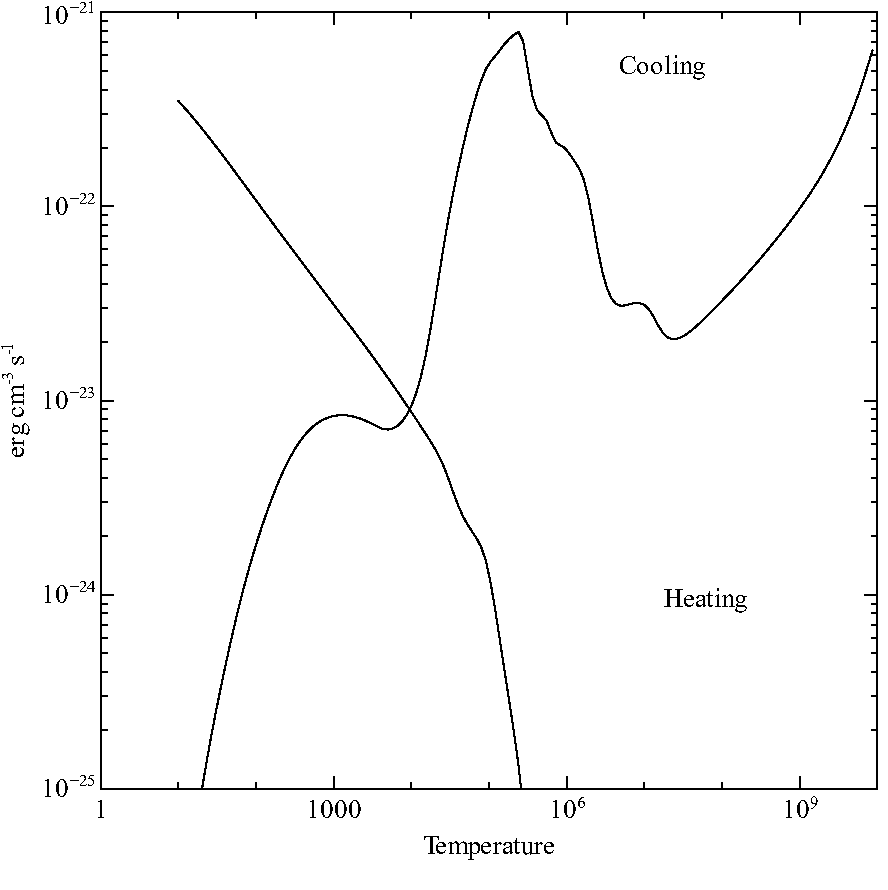
\includegraphics[scale=0.8]{cooling_heating}
\caption[Cooling and heating in a photoionized gas]{\label{fig:cooling_heating}A typical heating---cooling function for low density photoionized
gas. The cooling and heating rates (erg cm$^{-3}$ s$^{-1}$) are shown.  }
\end{figure}

Collisionally-ionized gas has a well-defined cooling rate that is only
a function of temperature.
The sample program
\cdFilename{hazy\_coolingcurve.cpp}
(included in the \cdFilename{programs} directory in the code's
distribution)  does such a
calculation, and Figure \ref{fig:coolcurve} shows the results.
Here the kinetic temperature
is set by some physics external to the calculation.
The entire ionization
solution is valid for each temperature under this assumption.
The
unspecified heat source would have to provide a local heating rate that
is equal to the calculated cooling rate for the solution to be time steady.

\begin{figure}
\centering
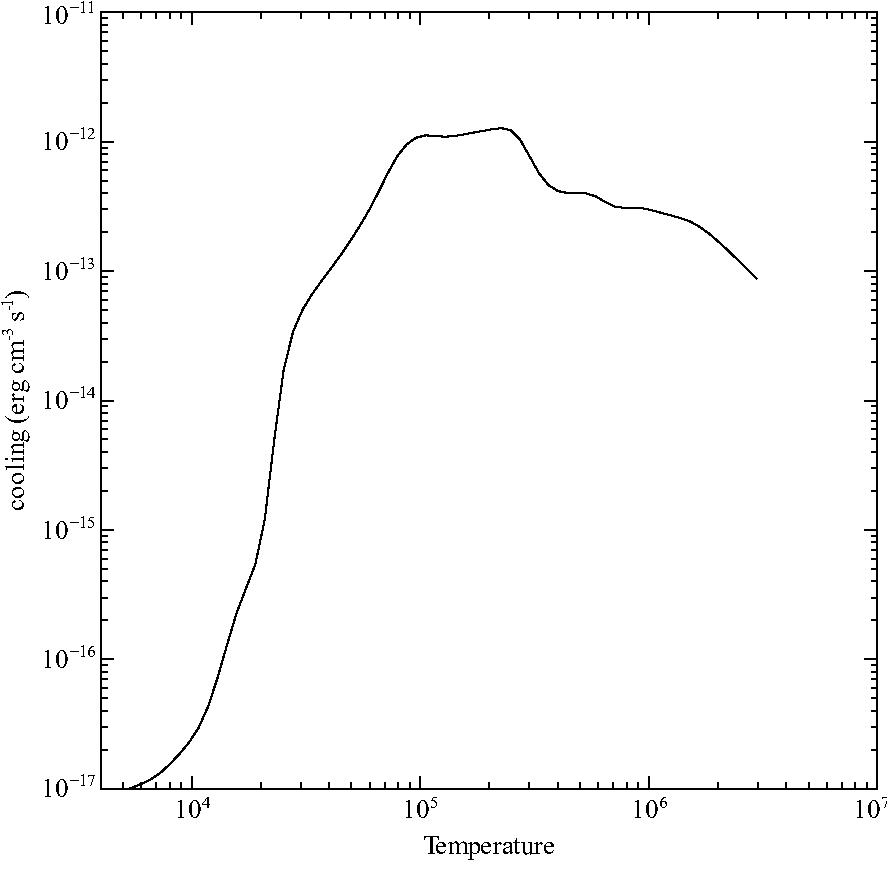
\includegraphics[scale=0.8]{coolcurve}
\caption[Cooling function for collisionally ionized gas]{\label{fig:coolcurve}A typical cooling function for low
density collisionally ionized gas.}
\end{figure}

The third map is the type of thermal stability map shown by \citet{Krolik1981} and plotted in Figure \ref{fig:hazy_kmt}.
The program that generated these
results is given in the file \cdFilename{hazy\_kmt.cpp}.
Here the equilibrium temperature
is determined self-consistently for gas over a wide range of densities,
but for a single flux of ionizing photons (or equivalently, distance from
the central object).

\begin{figure}
\centering
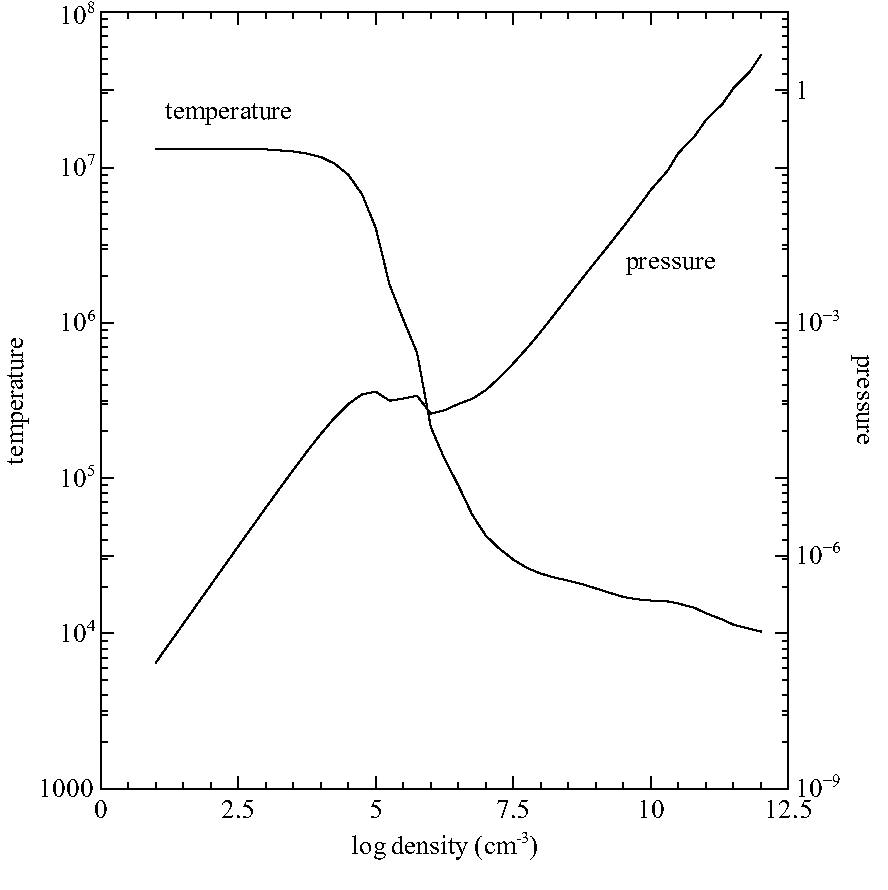
\includegraphics[scale=0.8]{hazy_kmt}
\caption[Temperature vs density in photoionization equilibrium]{\label{fig:hazy_kmt}Equilibrium temperature as a function of density.}
\end{figure}

\subsection{No Temperature Convergence}

A temperature failure occurs when the heating-cooling balance is not
within a certain tolerance,
set by the \cdCommand{set temperature error} command,
after 20 tries.
Normally \Cloudy\ will punt after an excessive number of temperature
failures occur.
The limit to the number of failures is reset with the
\cdCommand{failures} command.
If the \cdCommand{failures map} command is entered then the code
will first produce a map of heating-cooling space to give an indication
of where the equilibrium temperature should have been when excessive
failures occur.

Temperature failures most often occur for temperatures
in the range $10^2 \K$
to $4\times 10^3 \K$, and $10^5 \K$ to $10^6 \K$.
These are where the cooling function permits
more that one thermal solution (see, for example, \citealp{Williams1967}; \citealp{Dalgarno1972}).

Figure \ref{fig:cooling_heating} shows a typical cooling function for
gas in photoionization equilibrium.
A peak is reached at a temperature near $10^3 \K$.
This occurs
when the fine-structure lines are major coolants.
At lower temperatures
their cooling rate increases exponentially (as expected),
until roughly
$10^3 \K$, when their Boltzmann factors are near unity.
Above this temperature
their cooling rate is nearly proportional to the Coulomb focusing factor
$T^{-1/2}$, and the cooling \emph{decreases} until the temperature
is high enough for
optical forbidden lines to become important (at roughly $4000 \K$).
A similar
phenomenon occurs near the $\sim 10^5 \K$ to $10^6 \K$ peak in
the cooling function.

When failures occur because more than one temperature solution is
possible,  the reported failures are a physical (not numerical) problem.
\Cloudy\ will try to deal with this by forcing the temperature to
values below the peak in the cooling function.
Increasing the number of allowed failures
(with the \cdCommand{failures} command) to prevent the code from
stopping prematurely
is permissible as long as the global energy balance is preserved.
A warning
will be issued at the end of the calculation if the heating-cooling balance
is not preserved.

\subsection{Thermal Stability}

The thermal solution may be unstable when the temperature derivative
of the net cooling function (cooling minus heating) is negative (\citealp{Field1965}).
Possibly unstable solutions are indicated by a ``u'' just before the
equilibrium temperature in the zone printout.  The temperature derivative
is for isochoric (constant density), not isobaric (constant pressure),
conditions.  Comments are printed at the end of the calculation if possibly
unstable thermal solutions are present in the calculation.

\subsection{Thermal fronts}

Just as an ionization front is a region where the level of ionization
changes dramatically over a small scale, a thermal front occurs where the
temperature changes dramatically over a small scale.  This can be caused
by a real physical change of state of the gas such as those that occur near
the peaks in the cooling curve.
An example of a thermal front, taken from
\citet{FerlandFabian2002}, is shown in Figure \ref{fig:thermal_front}.
This type of jump is physical.
The gas changes phase and moves to different branches
of the cooling curve.
The code will generate a caution or comment if the
electron temperature changes discontinuously from one zone to the next.

\begin{figure}
\centering
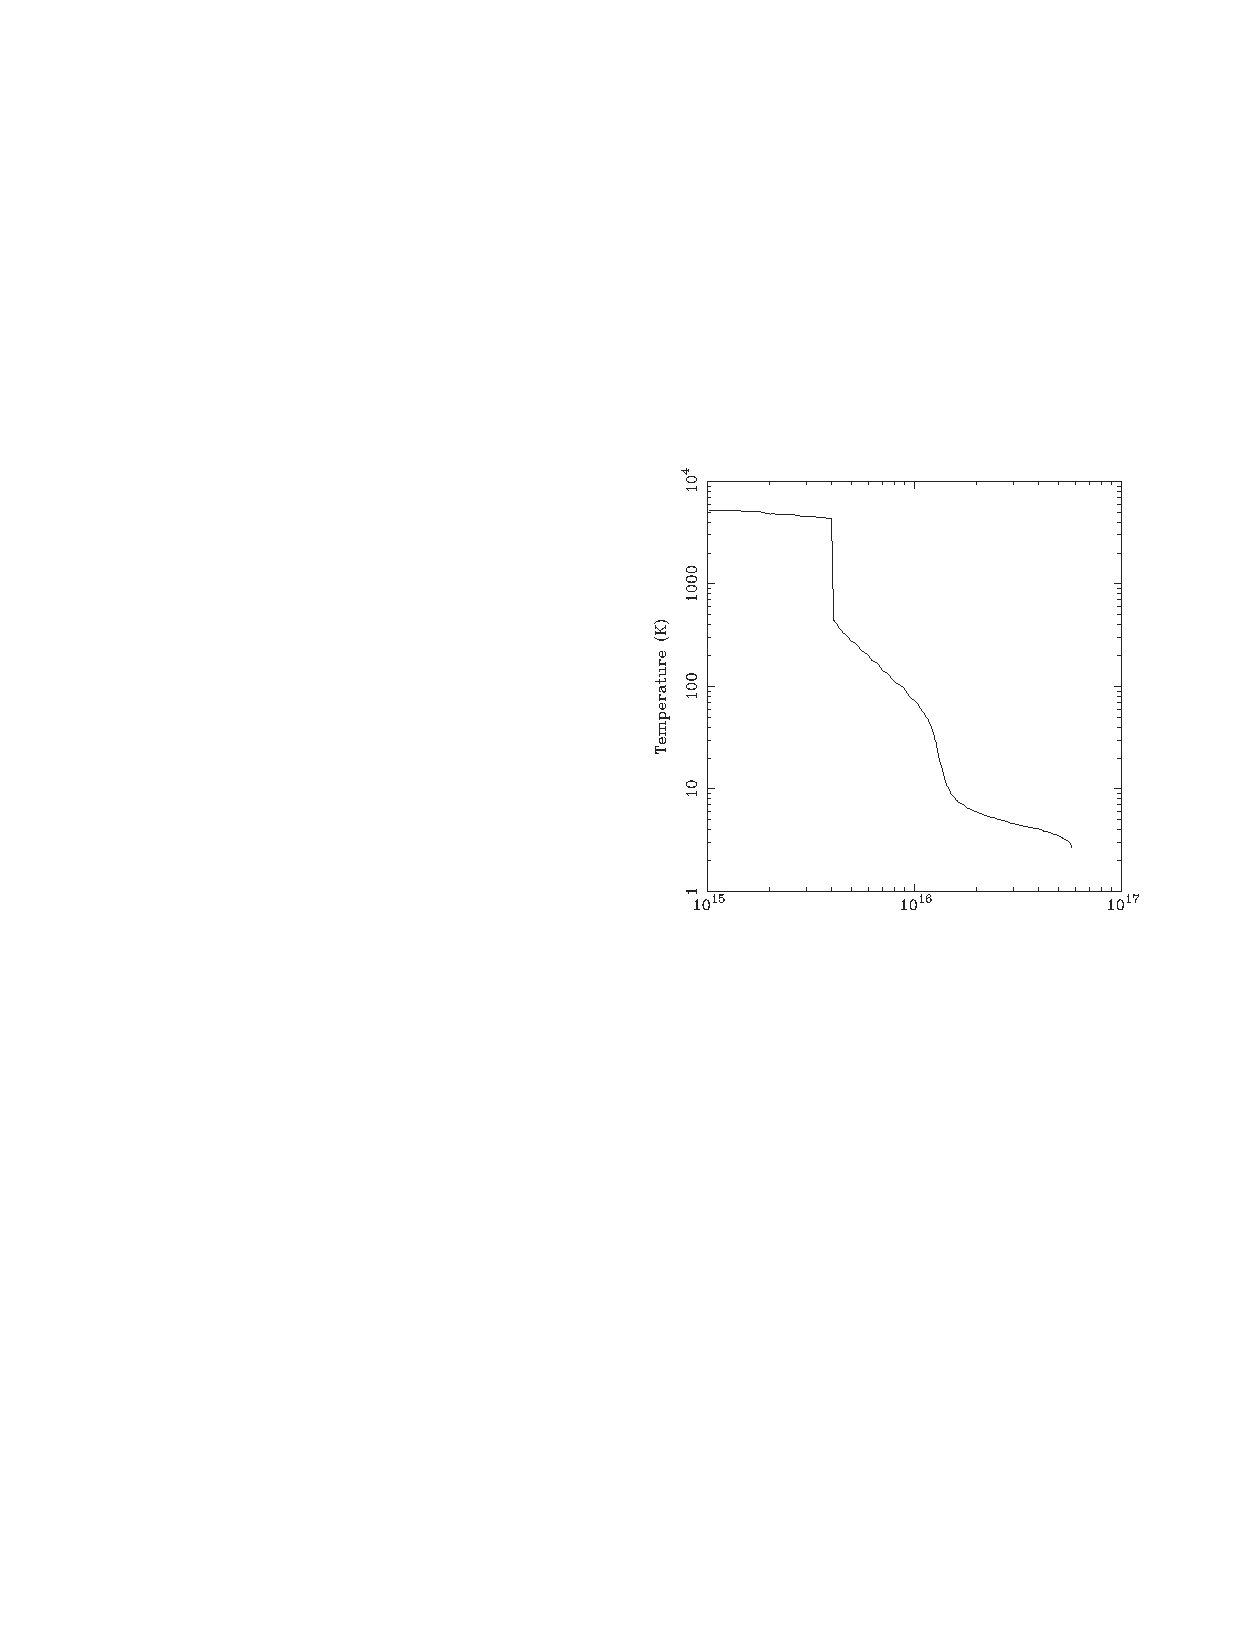
\includegraphics[scale=1.2]{thermal_front}
\caption[Thermal front example]{\label{fig:thermal_front}An example of a thermal front
in a cooling flow cloud
(\citealp{FerlandFabian2002}). The x-axis is the depth into the cloud (cm).
The thermal front at $\sim 4\times 10^{15}$~cm is unresolved.}
\end{figure}

A thermal front can lead to pressure convergence failures when the
solution jumps between the high and low temperature branches.
Figure \ref{fig:pressure_density}
shows an example case, taken from \cdFilename{orion\_hii\_pdr\_pp.in}
in the test suite.
This shows the pressure history (output with the
\cdCommand{save pressure history} command).
The solver adjusts the density trying to make the resulting
pressure agree with the desired pressure.
The pressure changes continuously
with density up to the point where the temperature jumps over the peak in
the cooling curve.
No solution is possible, and the code announces a
pressure failure.
In nature the presence of a magnetic field (added with
the \cdCommand{magnetic field} command) will cushion the front
from large changes in density.

\begin{figure}
\centering
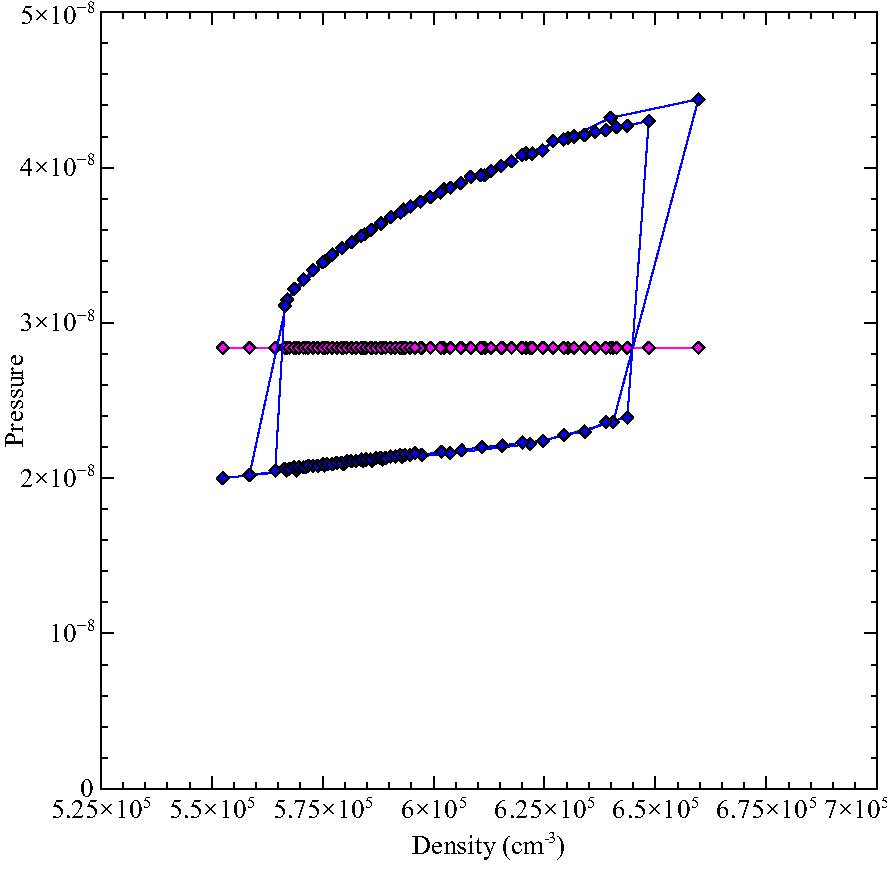
\includegraphics[scale=0.5]{pressure_density}
\caption[Thermal front]{\label{fig:pressure_density}A thermal front in a
constant pressure simulation.  The x-axis
gives the density [cm$^{-3}$] and the y-axis is the pressure
[dynes cm$^{-2}$].
The
points forming the large box are the resulting total gas pressure and the
horizontal line is the correct pressure.
The solution jumps above and below
the equilibrium value as the temperature jumps above and below the thermal
front.}
\end{figure}

A serious of pressure failures occur in this simulation when the gas
falls to a temperature of $\sim 300 \K$,
as shown in Figure \ref{fig:temperature_depth}.
The code simply
presses on with the goal of reaching the cold side of the front.

\begin{figure}
\centering
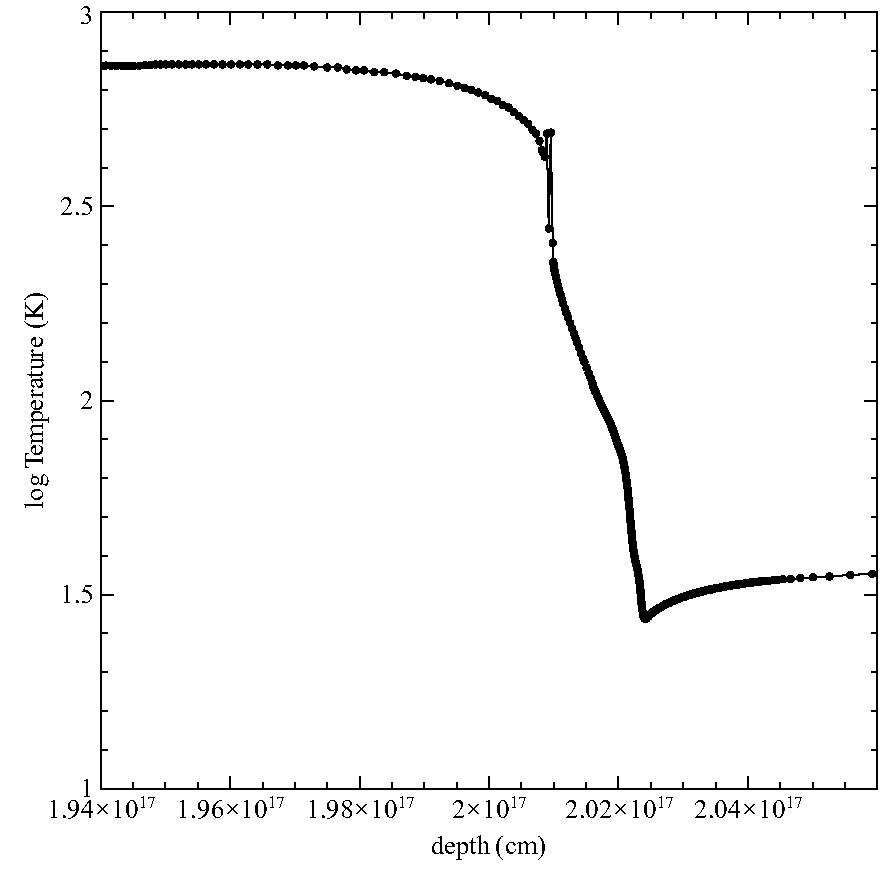
\includegraphics[scale=0.5]{temperature_depth}
\caption[Constant pressure thermal front]{\label{fig:temperature_depth}A constant-pressure thermal front
in a temperature - radius plot.
The x-axis gives the radius (cm).  The y-axis gives the log of the
temperature (K).
The solution jumps above and below the equilibrium value,
leading to a series of pressure failures, near a depth of
$2\times 10^{17}$~cm, as
it soldiers on through the thermal front.}
\end{figure}

\subsection{Map Output}

The program stops if an excessive number of temperature failures occur.
The default limit is 20.
It will produce a map of the heating and cooling
as a function of temperature for the last computed zone if the \cdCommand{map} option
on the \cdCommand{failures} command is given.
The map is described here.
The start
of the output from the test case \cdFilename{func\_map.in} is shown below.

\tiny
\begin{verbatim}
90.02x map of heating vs cooling
 te, heating, cooling.
 Cloudy punts, Te= 9.254E+03 HTOT= 9.123E-24 CTOT= 9.118E-24 nzone=   1
 COOLNG array is
     O  4    25  0.340 O  3  5007  0.182 O  3    88  0.075 H FB     0  0.057 S  4    10  0.048 O  3    51  0.042 S  3  9532 0.035
     H ff     0  0.022 S  3    33  0.020 Ne 3    15  0.019 Hefb     0  0.015 N  3    57  0.015 Ne 3  3869  0.013 S  3    18 0.013
     Ne 5    24  0.010 Ne 5    14  0.009 C  3  1910  0.008 Heff     0  0.007 Si 2    34  0.006 Fe 5  3892  0.006 O  2  3727 0.005
 Line heating array follows
    Te     Heat-------------------> Cool---------------------->    dH/dT    dC/DT       Ne         NH      HII       Helium
1.0000E+01 3.4774E-22   1   1 0.636 4.6095E-26 H FB    0A 0.723 -8.19E-24  1.56E-27 9.1178E-01 1.0000E+00 -0.07 -0.40 -0.24 -1.75
1.0209E+01 3.4490E-22   1   1 0.635 4.6814E-26 H FB    0A 0.720 -7.98E-24  1.65E-27 9.1353E-01 1.0000E+00 -0.07 -0.40 -0.23 -1.73
1.0423E+01 3.4233E-22   1   1 0.635 4.7510E-26 H FB    0A 0.717 -7.74E-24  1.74E-27 9.1491E-01 1.0000E+00 -0.07 -0.41 -0.23 -1.73
\end{verbatim}
\normalsize

The output begins with a listing of the strongest coolants for the last
zone.
Then the program steps through increasing temperatures and prints
the heating, cooling, and ionization of the gas.
From this information
it should be possible to determine the temperature where the equilibrium
thermal solution should have been.
Each solution is completely
self-consistent, except that heating and cooling do not balance.
Both the
local attenuated radiation field and collisional ionization contribute to
the ionization balance at each temperature.
All processes contribute to
the thermal balance, including collisional ionization.
The map is at
constant density.

The first column gives the temperature.
Columns 2 and 6 give the volume
heating and cooling.
Both have units erg s$^{-1}$ cm$^{-3}$.
Columns 3 and 4
constitute an indication of the main heating source.
Columns 7 and 8 give
the label and wavelength of the strongest coolant.
Columns 5 and 9 give
the fraction of the total heating or cooling due to these agents.
Columns
10 and 11 give the heating and cooling derivatives.
Columns 12 and 13 give
the electron and hydrogen densities (cm$^{-3}$) and the remaining columns give
the logs of the hydrogen and helium ionization fractions.
The location
of the probable thermal solution is indicated by a comment surrounded by
dashed lines.

\section{Convergence problems with dust-free static sphere}

Ionization convergence problems can occur with a dust-free static
spherical geometry.
The default geometry when the \cdCommand{sphere} command is entered
is for lines to freely escape after crossing the central hole due to some
level of expansion.
In a static spherical geometry (set with the
\cdCommand{sphere static} command) the total \la\ optical depth
at the illuminated face of the
shell will be very large since the line is scattered by the matter that
lies across the entire shell.
The line is destroyed when dust is present.
If dust is not present the \la\ intensity $J$ will become very large.  If the
total optical depth in \la\ is also large then the dominant escape /
destruction process for the line will be absorption by atoms of third-row
elements or the $n=2$ level of hydrogen.  This can lead to ionization
convergence problems due to the extremely large \la\ intensity $J$.

The first question to ask is whether this geometry is appropriate.  Dust
is nearly always present in the ISM.  In dense stellar environments it is
unlikely that a spherical geometry will be static.  Include dust, use the
default expanding spherical geometry, or a wind, and the problem will go
away.  To the best of my knowledge this geometry does not occur in nature.

\section{Optical depth convergence problems}

The code generally will not converge if it has not done so within ten
or so iterations.  Convergence problems most commonly occur when the
specified column density or thickness is very near a prominent ionization
front.  In this case very small changes in the physical conditions result
in large changes in the optical depths.
The code will not have convergence
problems if an optical depth is used as a stopping criterion instead.

\section{Negative populations}

It is possible that the code will stop because negative level populations
were predicted for atoms, ions, or molecules.
This is not supposed to occur,
but sometimes happens because of numerical instabilities in the matrix
inversion routine.
Please post the input stream and version of \Cloudy\ on
the code's discussion board.

\section{Floating Point Errors}

The code should be compiled and linked with options enabled so that the
code will crash on overflow or division by zero, but ignore underflow.
The \cdCommand{crash} command described in Part 1 tests this.  \emph{Floating point errors should never occur.}
The logic within the code is designed to identify
problems, and complain, but not fail.
The logic is only as good as the
tests they were designed to pass.
It is inevitable that circumstances will
occur for which the logic now in the code is not sufficient.
It is possible
that the code will fail when these circumstances occur.
I would be grateful
for reports of any such failures, since they inevitably identify shortcomings
in the code, and lead to its improvement.
Please post comments on the
discussion board on the code's web site.

\section{We can't fix it if we don't know it's broken}

Machines are growing faster far more rapidly than people are getting
smarter.
Reliability in the face of complexity is the major challenge to
the development of any large-scale computer code (\citealp{Ferland2001b}).  There
can be little doubt that \Cloudy\ contains bugs.

If problems arise or the code crashes then it is likely that you found
a problem.  We would appreciate learning about such problems since they
identify shortcomings which usually lead to improvements in the code (or
the documentation).  Please post queries and bug reports on the discussion
board on the code's discussion board.
     %proof 1
\chapter{HISTORY AND ACKNOWLEDGEMENTS}
% !TEX root = hazy2.tex

\section{History}

\Cloudy\ was born at the Institute of Astronomy, Cambridge, in August of
1978, in the computing environment described in the web document
\href{http://www.nublado.org/gary/computing1970s.htm}{http://www.nublado.org/gary/computing1970s.htm}.  Its development has been
continued at The University of Kentucky, The Ohio State University, and
during extended visits to the Joint Institute for Laboratory Astrophysics,
the Royal Greenwich Observatory, IOA Cambridge, Cerro Tololo Interamerican
Observatory, and the Canadian Institute for Theoretical Astrophysics.

The code has been through three computer languages.  It was originally
written in FORTRAN IV and advanced through several dialects,
reaching FORTRAN
77  in 1994 (version 84). Version 90 was written in a mix of FORTRAN 77
and MILSPEC extensions.  This was the most advanced Fortran that could be
used with open source compilers.  It moved to ANSI 89 C in 1999 (version
96) and to C++ with the release of 07.02 in 2007.

Moore's Law is due to Gordon Moore, one of the founders of Intel
Corporation.  He observed that modern CPU's become about twice as powerful
every 18 months.  This trend has held true for the past twenty years, shows
no sign of failing, and seems to be associated with our ability to control
complexity.  By this standard the growth of \Cloudy\ has been conservative,
in that it is growing slower and complex on the Moore's-law timescale.
Figure \ref{fig:size} shows the evolution of the code,
as indicated by its size as a
function of time.\footnote{Before mid-1995 the size was the total number of lines in the
distributed source.  After 1995 the size only includes the number of lines
excluding block data.  When the code was converted to C the block data
were converted to external data files.  These external files are now far
larger than the code itself.}
As another example, the Meudon 1985 Meeting planetary
nebula test (\cdCommand{pn\_paris.in} in the test cases)
has always taken about one minute to compute.

\begin{figure}
\centering
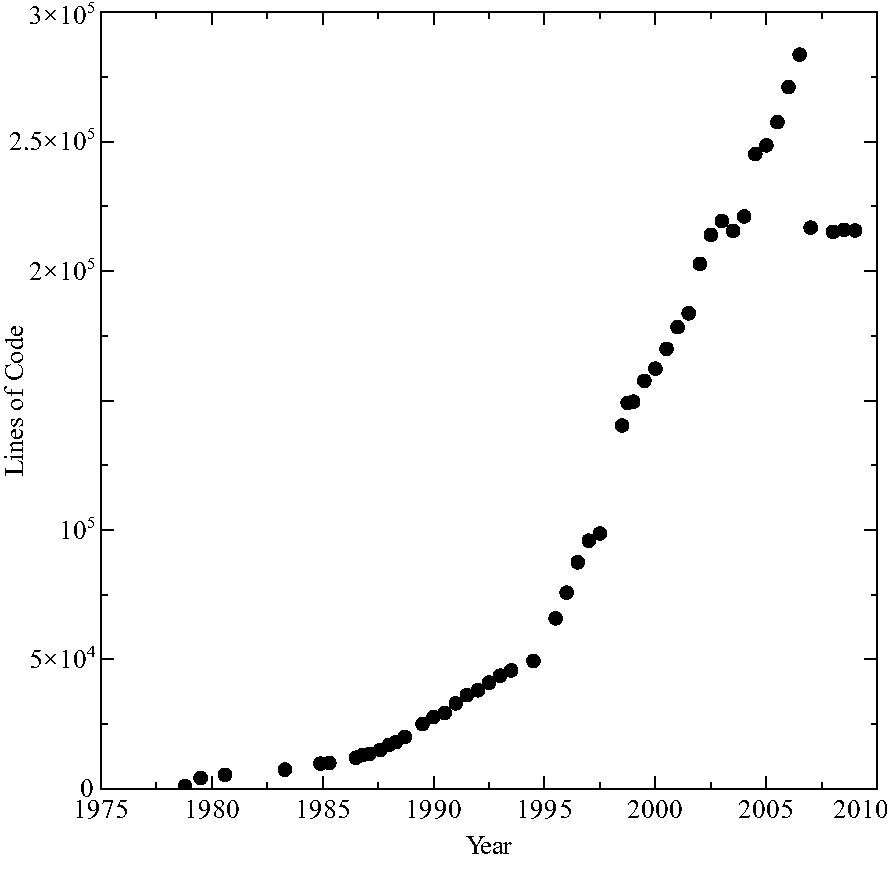
\includegraphics{size}
\caption[\Cloudy's size vs time]{\label{fig:size}The size of the code as a function of time. The code grows roughly
7\% larger per year, with growth spurts and slowdowns at times. There are
several changes in slope evident - the year and cause are: 1985 - mainframe
to Unix; 1993 - Unix to windows; the jump at 1999 - the Fortran to C
conversion and the Williams / van Hoof drop in 2006, due to the use of
object-like structures and moving converted fortran block data into separate
files.}
\end{figure}

\section{Acknowledgments}

Comments or suggestions which led to the improvement of \Cloudy\ were made
by the many individuals acknowledged on the web site
\href{http://www.nublado.org}{http://www.nublado.org}.

Peter G. Martin and Hagai Netzer had special roles during the early
development of the code.  Peter added several of the commands that deal
with ordering of supplemental line lists and the luminosity options on the
\cdCommand{blackbody} command, insisted that \Cloudy\ run on a VAX, provided access to
the University of Toronto VAX 11/780 during the 1980's, and more recently
hosted the group at CITA during a sabbatical.  Hagai and I have spent
countless hours arguing over methods, assumptions, and just whose code had
the bug.  These comparisons are the only way to debug codes as large as
\Cloudy\ or ION.

Peter van Hoof has gone over the code very carefully, finding many
problems, and expanding its capabilities.  The current version of the grain
physics was developed by Peter together with Peter Martin, and Joe
Weingartner.  PvH developed the stellar library implementation in the current
version.  He is the maintainer for both the grains and stellar atmospheres
codes.

The move to make the solvers far more rigorous and include dynamics and
advection has been led by Robin Williams and Will Henney.  Robin has
rewritten the chemistry solvers to take advantage of the structures present
in the C language and make them more robust.

The initial implementation of the hydrogen iso-electronic sequence was
done by Jason Ferguson as part of his thesis. Ryan Porter developed the
He-like isoelectronic sequence in his thesis. The expansion of the
simulations into the PDR was done by Nick Abel and Gargi Shaw as part of
their theses.

Sections of the code are taken from public domain software, as
acknowledged in this document and in the source.
Portions of the code were written by those listed in the
\cdFilename{others.txt} file in the distributed files.

The preparation of the bibliographic references in this document made
use of data from the NASA's Astrophysics Data System Bibliographic
Services.

The development of \Cloudy\ would not have been possible without
twenty nine years of continuous support by The National Science
Foundation.  This began with AST 80-2522, and has been continued with
grants 83-05094, 85-12414, 87-19607, 90-19692, 93-19034, 96-17083,
00-71180, 03-0772, and most recently AST 06-07028.  NASA has supported
\Cloudy\ through ATP program awards NAG5-12020 and NNG05GD81G.
Support from the University of Kentucky Center for Computational
Sciences is also gratefully acknowledged.

      %proof 1
\appendix
\chapter{ATOMIC DATA SOURCES}
% !TEX root = hazy2.tex

Codes like \Cloudy\ can only exist because of the large body of work 
done by the atomic and molecular physics community.
This work will only continue
to be supported if it is cited in the literature whenever it is used.
The
following is a partial list of citations for the atomic data used within
the code.

This table is generated by the perl script \cdFilename{doc\_atomic\_data.pl}.
This generates the file \cdFilename{doc\_atomic\_data\_refer.txt}
which is pasted below.

      %proof 1
\chapter{GLOSSARY OF SYMBOLS}
% !TEX root = hazy2.tex

As far as possible, the notation used by \Hazy\ follows
standard texts (AGN3; \citealp{Mihalas1978}).
This is a summary of some of the symbols used.

The fundamental constants used by the code are from the
\href{http://physics.nist.gov/cuu/Constants/index.html}{
CODATA recommended values}.
Constants are contained in the header \cdFilename{physconst.h}.

\begin{tabbing}
  \textbf{Symbol}\quad \= \textbf{Description}\hspace{10em} \= \textbf{Units}\hspace{8em} \=
  \textbf{Notes}\quad\quad \\
  $a$ \>  Stefan radiation density \>   erg cm$^{-3}$ K$^{-4}$ \>
$7.56464\times 10^{-15}$\\
$a$ \>  damping constant \>   ---\\
$a_o$ \>  Bohr radius \>  $\hbar
/{m_e}{c^2}$ cm \>  $0.5291775\times 10^{-8}/Z$\\
$A_{rad}$ \>   radiative acceleration \>  cm s$^{-2}$\\
$A_{ul}$ \>  radiative rate from level $u$ to $l$ \>  s$^{-1}$\\
 $b_n$ \>  departure coefficient \> ---\\
$B$ \>  magnetic field \>  esu \>  \\
$B_\nu$ \>  Planck function \>  erg cm$^{-2}$ s$^{-1}$ Hz$^{-1}$ sr$^{-1}$\\
$c$ \>   speed of
light \>  cm s$^{-1}$ \>   $2.997925\times 10^{10}$\\
$C$ \>  collisional rate \>  s$^{-1}$\\
$C_{ul}$ \>  line collision rate \>  s$^{-1}$\\
$D_{ul}$ \>  line destruction probability \> ---\\
$f$ \>  oscillator strength\> ---\\
$f(r)$ \>  filling factor \> --- \> \\
$f_\nu$ \>  flux density \>  erg cm$^{-2}$ s$^{-1}$ Hz$^{-1}$\\
$F_\nu$ \>  flux density \>  erg s$^{-1}$
Hz$^{-1}$\\
$g$ \>  grain asymmetry factor \> ---\\
$g_i$ \>  statistical weight \> ---\\
$g_{III}$ \>  T
aver free-free gaunt factor \> ---\\
$g_/$ \>  Solar surface gravity \>  cm
s$^{-2}$ \>  $2.74\times 10^4$\\
$G$ \> gravitational constant \>  dyne cm$^2$ g$^{-2}$ \>  $6.673\times 10^{-8}$\\
$G$ \>  energy gains,
heating \>  erg cm$^{-3}$ s$^{-1}$\\
$h$ \>  Planck's constant \>  erg s \>  $6.6262\times 10^{-27}$\\
$\hbar $ \>  Planck's constant \>  erg s \>   $1.0546\times 10^{-27}$\\
$I$ \>  integrated intensity \>  erg s$^{-1}$ sr$^{-1}$ Hz$^{-1}$\\
$I_n$ \>  ionization potential of level n \>   erg Ryd\\
$I_\nu$ \>  intensity \>  erg s$^{-1}$ sr$^{-1}$ Hz$^{-1}$\\
$J$ \>  integrated mean intensity \>  erg s$^{-1}$ sr$^{-1}$\\
$J_\nu$ \>  mean intensity \>  erg s$^{-1}$ sr$^{-1}$ Hz$^{-1}$\\
$k$ \>  Boltzmann constant \>  eV deg$^{-1}$ \> $8.6171\times 10^{-5}$\\
$k$ \>  Boltzmann constant \>  erg deg$^{-1}$ \>  $1.38062\times 10^{-16}$\\
$L_\odot$ \>  luminosity of sun \>  erg s$^{-1}$ \>  $3.826\times10^{33}$\\
$m_A$ \>  mass  of atom A \>  gm\\
$m_{\mathrm{AMU}}$ \>  atomic mass unit \>  gm \>  $1.6605402\times10^{-24}$\\
$m_e$ \>  electron mass \>  gm \>  $9.10956\times 10^{-28}$\\
$m_e$ c$^2$ \>  electron energy \>  Ryd \>  $3.75584\times10^4$\\
$m_p$ \>  proton mass \>  gm \>  $1.6726231\times 10^{-24}$\\
$M_J$ \>  Jeans' mass \>  gm\\
$M_\odot$ \>  mass of the sun \>  gm \>  $1.989\times 10^{33}$\\
$M_\oplus$ \>  mass of the Earth \>  gm \>  $5.977\times 10^{27}$\\
$n_e$ \>  electron
density \>  cm$^{-3}$\\
$n_j$ \>  population of level $j$ \>  cm$^{-3}$\\
$n_p$ \>  proton density \> cm$^{-3}$\\
$n(H)$ \>  total
H density, all forms \>  cm$^{-3}$\\
$n(x)$ \>  density of species x \>  cm$^{-3}$\\
$n(cr)$ \>  cosmic ray
density \>  cm$^{-3}$\\
$n$ \>  atom's level \> --- \\
$n(\mathrm{H}_{tot})$ \>  H density, all forms \>  cm$^{-3}$\\
$N$(x) \>  column density
of species x \>  cm$^{-2}$\\
$N(\mathrm{H}_{tot})$ \>  total H col den, all forms \>   cm$^{-2}$\\
$N_{\mathrm{eff}}$ \>  effective H
column density \>  cm$^{-2}$\\
$ P*$(x) \>  LTE relative population \>  cm$^3$\\
$P_{gas}$ \>  gas pressure \>  dyn
cm$^{-2}$\\
$P_{lines}$ \>  line radiation pressure \> dyn cm$^{-2}$\\
$P_{tot}$ \>  total pressure \>  dyn cm$^{-2}$\\
$P_{ul}$ \>  line
escape probability \> ---\\
$P_{\tau x}(n)$ \>  continuum escape prob \> ---\\
pc \>  parsec \>  cm \>  $3.085678\times 10^{18}$\\
$q_{ij}$ \>  line collisional rate coefficient \>  cm$^3$ s$^{-1}$\\
$q_n$ \>
collisional rate coefficient \>  cm$^3$ s$^{-1}$\\
$q_e$ \>  electron charge \>   esu \>
$4.80325\times 10^{-10}$\\
$Q_{\mathrm{abs}}$ \>  grain absorption efficiency \> ---\\
$Q$(H) \>  hydrogen ionizing photons \>
s$^{-1}$\\
$r$ \>  radius \>  cm\\
$r_{l,u}$ \>  rate \>  s$^{-1}$\\
$R_0$ \>  inner radius \>  cm\\
$R$ \>  total to selective extinction \> ---\\
$R_{\mathrm{H}}$ \>  Rydberg unit for H \> ---\\
$R_\infty$ \>  Rydberg unit for inf mass \> ---\\
$R_{\mathrm{AU}}$ \>  radius of Earth's orbit \>  cm \>  $1.4959\times 10^{13}$\\
$R_+$ \>  radius of the
Earth \>  cm \>  $6.378\times10^{18}$\\
$R_\odot$ \>  radius of the sun \>  cm \>  $6.9599\times 10^{10}$\\
$T_e$ \>  electron temperature \>
cm$^{-3}$\\
$T_{eff}(\odot)$ \>  Sun's effective temperature \>  K \>  $5770 \K$\\
$T_{exc}$ \>  excitation
temperature \>  K \> \\
$T_{color}$ \>  color temperature \>  K\\
$T_{low}$ \>  lowest temp allowed \>  K \>   \TEMPLIMITLOW\\
$T_{u}$ \>  energy density temperature \>  K\\
$u$ \>  energy density \>  erg cm$^{-3}$\\
$U_g$ \>  grain
potential \>  volt\\
$u$ \>  velocity (mean or projected) \>  cm s$^{-1}$\\
$\bar u$ \>  mean particle speed \>  cm s$^{-1}$\\
$u_{Dop}$ \>  Doppler velocity \>  cm s$^{-1}$\\
$u_{exp}$ \>  expansion
velocity \>  cm s$^{-1}$\\
$u_{th}$ \>  thermal velocity \>  cm s$^{-1}$\\
$u_{turb}$ \>  turbulent velocity \>  cm s$^{-1}$\\
$V_g$ \>  grain potential \>  eV\\
$V_n$ \>  grain work function \>  eV\\
$W$ \>  geometric dilution factor \> ---\\
$x$ \>  relative shift from line center \> ---\\
$X_c$ \>  continuous to total opacity \> ---\\
$\hat Y$ \>
grain photoelectric yield \> ---\\
year \>  \>  s \>  $3.156\times 10^7$\\
$z$ \>  redshift \> ---\\
$Z$ \> nuclear
charge \> ---\\
$\alpha$ \>  Fine structure constant \>  $q_e^2/( {\hbar c} )$ \>
1/137.036\\
$\alpha(n, T)$ \>  recombination coefficient \>  cm$^3$ s$^{-1}$\\
$ \bar \alpha (n,T)$ \>
effec recomb coefficient \>  cm$^3$ s$^{-1}$\\
$\alpha_\nu$ \>  continuous abs cross section \>
cm$^2$\\
$\alpha_{lu}$ \>   line absorption cross section \>  cm$^2$\\
$\alpha_\beta$ \>  Case B recomb rate coef \>  cm$^3$
s$^{-1}$\\
$\beta$ \>  recombination cooling coef \>  cm$^3$ s$^{-1}$\\
$\eta_\nu$ \>  photon occupation number \> ---\\
$\delta r$ \>  zone thickness \>  cm\\
$\Delta r$ \>  depth into cloud \>  cm\\
$\gamma_u,l$ \>  continuum pumping probability \> ---\\
$\Gamma_n$ \>  photoionization rate \>  s$^{-1}$\\
$\Gamma$ \>  reciprocal
lifetime of up level \>  s$^{-1}$\\
$\Gamma_{OTS}$ \>  OTS photoionization rate \>   s$^{-1}$\\
$\kappa$ \>  absorption opacity \>
cm$^{-1}$\\
$\kappa_{lu}$ \>  line absorption opacity \>  cm$^{-1}$\\
$\kappa_s$ \>  continuous scattering opacity \>  cm$^{-1}$\\
$\kappa_\nu$ \>  continuous absorption opacity \>  cm$^{-1}$\\
$\lambda_J$ \>  Jeans' length \>   cm\\
$\Lambda$ \>  energy loss,
cooling \>  erg cm$^{-3}$ s$^{-1}$\\
$\mu$ \>  mean molecular weight \> ---\\
$\Omega$ \>  energy-specific collision strength \> --- \\
$\Omega$ \>  shell coverage \>  sr\\
$\Omega/4\pi$ \>  covering factor \> ---\\
$\Phi$(H) \>  flux of ionizing
photons \>   cm$^{-2}$ s$^{-1}$\\
$\phi\nu$ \>  photon flux density \>  cm$^{-2}$ s$^{-1}$ Ryd$^{-1}$\\
$\phi_{OTS}$ \>  flux of OTS photons \>
cm$^{-2}$ s$^{-1}$\\
$\rho$ \>  mass density \>  gm cm$^{-3}$\\
$\pi a_o^2$ \>  area of first Bohr
orbit \>  cm$^2$ \>  $87.9737\times10^{-18}$\\
 \> Classical electron radius \> $q_e^2/( {{m_e}{c^2}}
)$
 cm \>  $2.818\times10^{-13}$\\
$\sigma_T$ \>  Thomson cross section \>  $8\pi /3 \times {\left[ {q_e^2/(
{{m_e}{c^2}})} \right]^2}$ \>
 $6.6524\times 10^{-25}$\\
 \>  \> cm$^2$\\
$\sigma_\nu$ \>  scattering cross section \>   cm$^2$\\
$\sigma_{\mathrm{Ray}}$ \>  Rayleigh scat cross section \>  cm$^2$\\
$\sum$ \>  projected grain area \>  cm$^2$\\
$\tau$ \>  optical depth \> ---\\
$\tau_{abs}$ \>
absorption optical depth \> ---\\
$\tau_{scat}$ \>  scattering optical depth \> ---\\
$\tau_{u,l}$ \>  line
optical depth \> ---\\
$\Upsilon$ \>  thermal averaged collision strength\> --- \\
$\nu$ \>  frequency \>  Hz\\
$\nu_{\mathrm{Ryd}}$ \>
frequency \>  Ryd\\
$\delta_\nu$ \>  line width \> Hz\\
$\delta\nu_{\mathrm{Dop}}$ \>  Doppler width \>  Hz\\
$\chi_s$ \>  h$\nu$/kT \> ---\\
\end{tabbing}
     %proof 1
\chapter{CONVERSION FACTORS}
% !TEX root = hazy2.tex

Table \ref{tab:ConversionFactors} gives conversion factors between
various common units.
The last column of the table gives the variable names for
constants that occur within the code.
Most are defined as macros within the header file
\cdCommand{physconst.h}.
These should be used instead of entering the constant directly.
In the following all Rydbergs are for infinite mass nuclei.

The fundamental constants used by the code are from the
\href{http://physics.nist.gov/cuu/Constants/index.html}{CODATA
recommended values}
and are in the header file \cdFilename{physconst.h}.
Derived quantities should be
formed from the fundamental quantities given there, so that any future
changes will trickle down into all parts of the code.

\begin{table}\caption{Conversion Factors}
\label{tab:ConversionFactors}
{\small
\begin{tabular}{lllll}
\hline
To convert from& Variable& to& multiply by& Parameter\\
\hline
AU&&cm& 1.49597870(13)&\\
Boltzmann
constant& BOLTZMANN& 1.3806503(-16)\\
cm&& micron($\mu$m)& $10^4$\\
phot/s/cm$^2$& flux& f$_\nu$& $\nu_{\mathrm{Ryd}}$h$\nu_1$ (erg)\\
phot/Ryd/s/cm$^2$& flux/widflx& $\nu f_\nu$& $\nu_{\mathrm{Ryd}}^2$ h$\nu_1$
(erg)\\
phot/Ryd/s/cm$^2$& flux/widflx& J$_\nu$& $\nu_{\mathrm{Ryd}}$ h\\
optical depth& tautot& A$_{\mathrm{V}}$(mag)& 1.08574\\
energy
(eV)&&  ergs& 1.602192($-$12)\\
energy (eV)&& K& 1.1604448(4)&\cdVariable{ eVdegK}\\
energy (keV)&& Frequency
Hz& 2.41799($+$17)\\
energy (Ryd)& anu& Kelvin& 1.5788866(5)& \cdVariable{Te1ryd}\\
energy
(Ryd)&anu& ergs& 2.179874($-$11)& \cdVariable{en1ryd}\\
energy (Ryd)& anu& cm$^{-1}$& 109737.315& \cdVariable{1/WavNRyd}\\
energy
(Ryd)& anu& eV& 13.6056981& \cdVariable{evRyd}\\
energy (Ryd)& anu& \AA& 911.6/energy(Ryd) & \cdVariable{rydlam}\\
energy (Ryd), T& anu,
Te& h$\nu$/kT& 1.5788866(5)*anu/Te& \cdVariable{Te1ryd}\\
temperature (K)& Te& eV& 8.617385($-$5)\\
temperature
(K)& Te& ergs& 1.38063($-$16)& \cdVariable{boltzmann}\\
temperature (K)& Te& Rydbergs& 1/1.5788866(5)&
\cdVariable{1/te1ryd}\\
wavelength (\AA )&& meters& 1(-10)\\
wavelength (\AA )&& ergs& 1.9864(-8)/$\lambda$(\AA)\\
wavelength (\AA )&& degree K& 1.43877($+$8)/$\lambda$(\AA )\\
wavelength
(cm)& micron& 1($+$4)\\
wavelength (cm)& \AA& 1($+$8)\\
wavelength
(cm)&& ergs& 1.9864($-$12)/$\lambda$(cm)\\
wavelength (cm)&& degree K& 1.43877/$\lambda$(cm)\\
wavelength
(cm)&& Rydbergs& 9.11256($-$6)/$\lambda$(cm)\\
wavelength (micron)&& degree
K& 1.43877($+$4)/$\lambda(\mu)$\\
wavelength (micron)&& ergs& 1.9864($-$12)/$\lambda(\mu)$\\
wavenumbers (
cm$^{-1}$)&& ergs& 1.98648($-$16)\\
wavenumbers ( cm$^{-1}$)&& degree K& 1.43877& \cdVariable{WavNKelv}\\
wavenumbers
( cm$^{-1}$)&& Rydbergs& 9.1126732($-$6)& \cdVariable{WavNRyd}\\
\hline
\end{tabular}
}\end{table}
   %proof 1
\chapter{THE TEST SUITES}
% !TEX root = hazy2.tex

\section{Introduction}

The code must be completely tested every time anything is changed.
This is done with the test suite that is included in the distribution.
The following pages list the test cases included in the \cdFilename{auto} directory
within the test suite directory \cdFilename{tsuite}.

The test suite contains a series of Perl scripts that automate several tasks.
The \cdFilename{readme\_tests.htm} file included with the tests
describes these scripts.
The script \cdFilename{doc\_tsuite.pl} extracts the test names
and the description of each, and creates two files,
\cdFilename{doc\_tsuite.htm}, a formatted description of each test,
and \cdFilename{doc\_tsuite.txt}, the table that
follows this discussion.

The test cases include a large number of \cdCommand{monitor} commands that allow the code to be
automatically tested every night.
These \cdCommand{monitor} commands have been removed from the examples below.

The simulations form various classes. The names of the classes and their intention
is given in Table \ref{tab:ClassesOfSimulations}.

\begin{table}
\centering
\caption{\label{tab:ClassesOfSimulations}
Keywords used in the Test Suite.}
\begin{tabular}{ c c  }
\hline
Class & Function \\
\hline
Blr & Broad emission line region of AGN \\
Coronal & Collisionally ionized gas with pre-set temperature \\
Dynamics & Flow \\
Function & Test various functions of the code \\
Geometry & Test geometric aspects, aperture command \\
HII & H II regions \\
IGM & Intergalactic medium \\
ISM & Interstellar medium \\
Limit & Test limiting cases \\
NLR & Narrow-lined region of AGN \\
Nova & Aspects of the classical nova explosion \\
Optimizer & Test the optimizers \\
PDR & Photodissociation region \\
PN & Planetary nebulae \\
Stars & Stellar atmospheres \\
\hline
\end{tabular}
\end{table}


\section{Organization of commands}

Commands can occur in any order but we have made an effort to
enter them in the following order.
This is so that they can be studied to see examples of how to
use the code.

\emph{c commands controlling continuum}

\emph{c commands for density \& abundances}

\emph{c commands controlling geometry}

\emph{c other commands for details}

\emph{c commands controlling output}
As indicated, there are the \cdCommand{print} and \cdCommand{save} commands
which control the code's output.

\emph{c commands giving the monitors}
Each test includes a number of \cdCommand{monitor} commands.
These give values of predicted quantities that the code has
obtained in the past.
Changes to the code may cause predicted values to change,
and if they do the \cdCommand{monitor} command will
announce it.

\section{The Auto Test Suite}

Table \ref{tab:AutoSimulationList} lists the simulations in the 
\cdFilename{auto} test directory.

\begin{table}
\centering
\caption{
The simulations in the auto test suite.}
\begin{tabular}{ c c  }
\hline
Class & Function \\
\hline
\input{../../../tsuite/auto/doc_tsuite.txt}
\hline
\label{tab:AutoSimulationList}
\end{tabular}
\end{table}

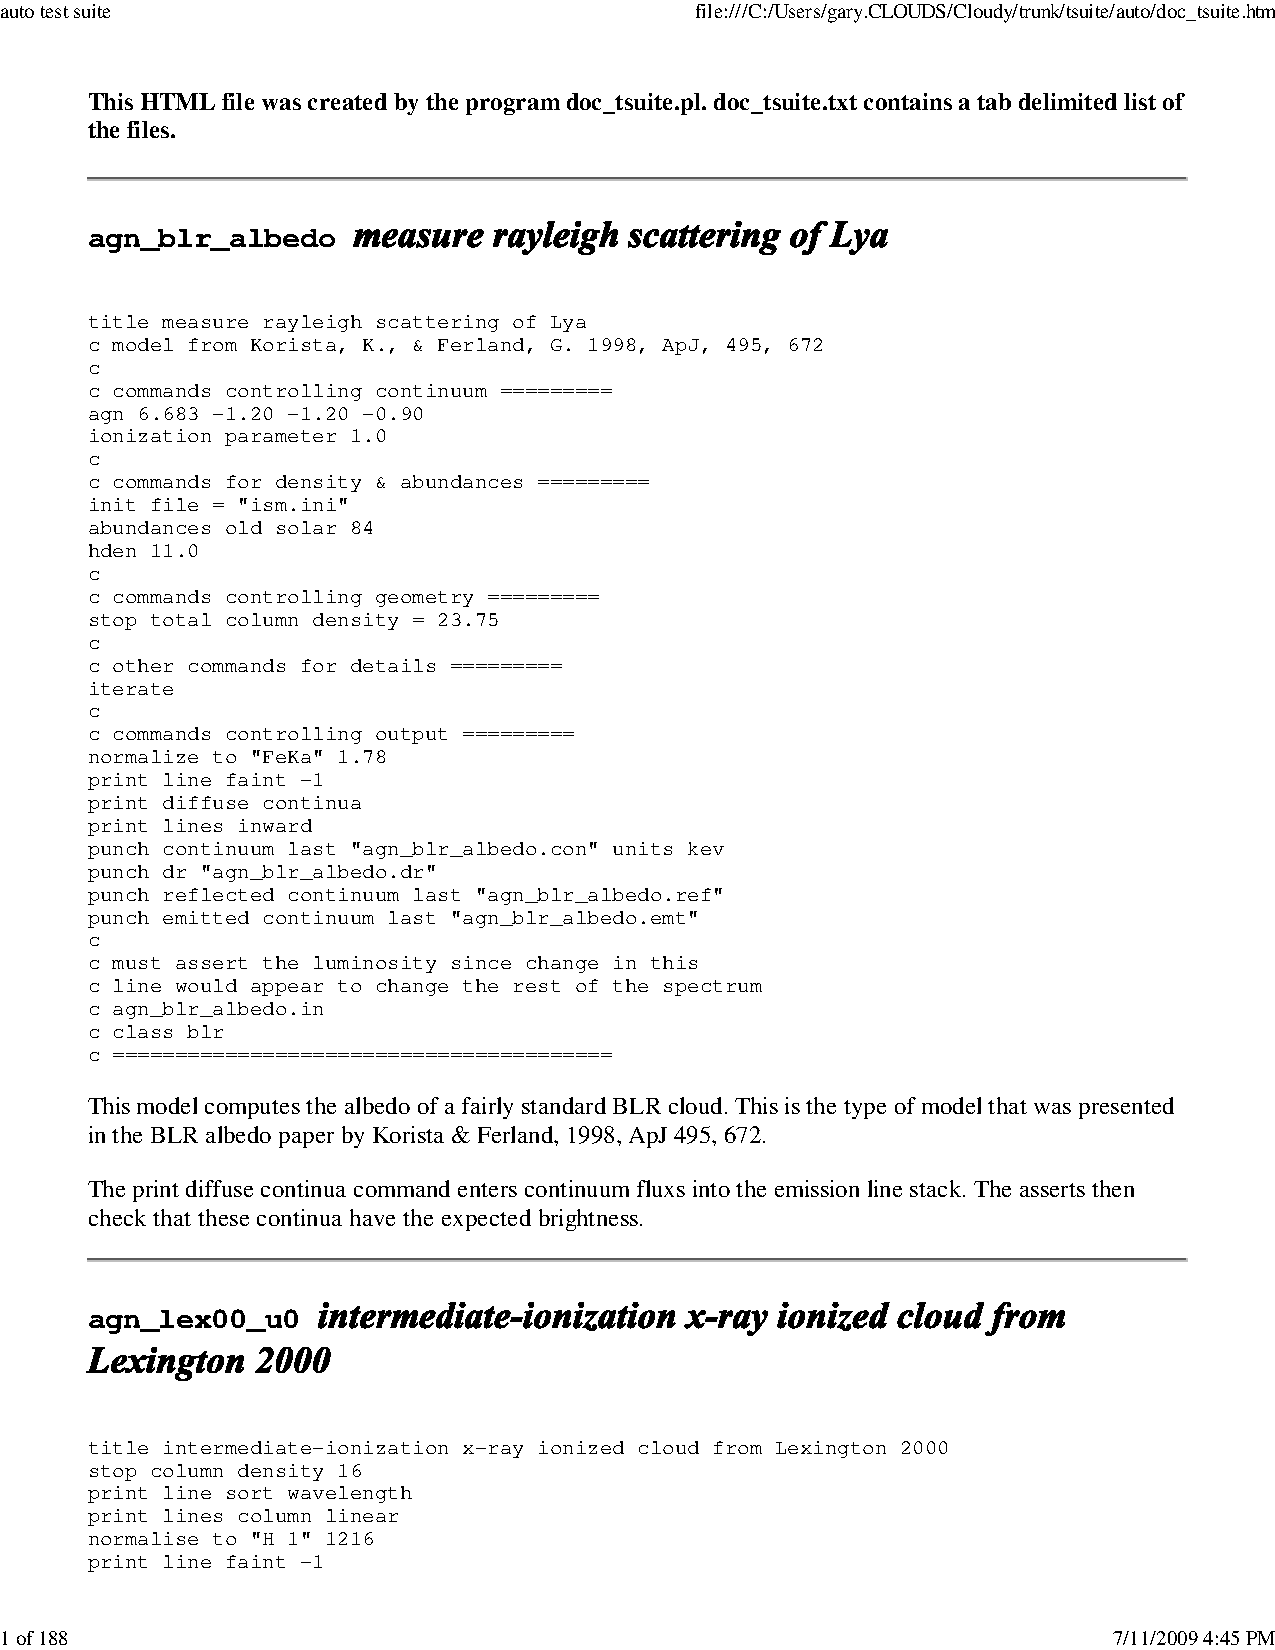
\includepdf[pages=-]{../../../tsuite/auto/doc_tsuite.pdf}

\section{The Slow Test Suite}

Table \ref{tab:SlowSimulationList} lists the simulations in the
\cdFilename{slow} test directory.

\begin{table}
\centering
\caption{
The simulations in the slow test suite.}
\begin{tabular}{ c c  }
\hline
Class & Function \\
\hline
\input{../../../tsuite/slow/doc_tsuite.txt}
\hline
\label{tab:SlowSimulationList}
\end{tabular}
\end{table}

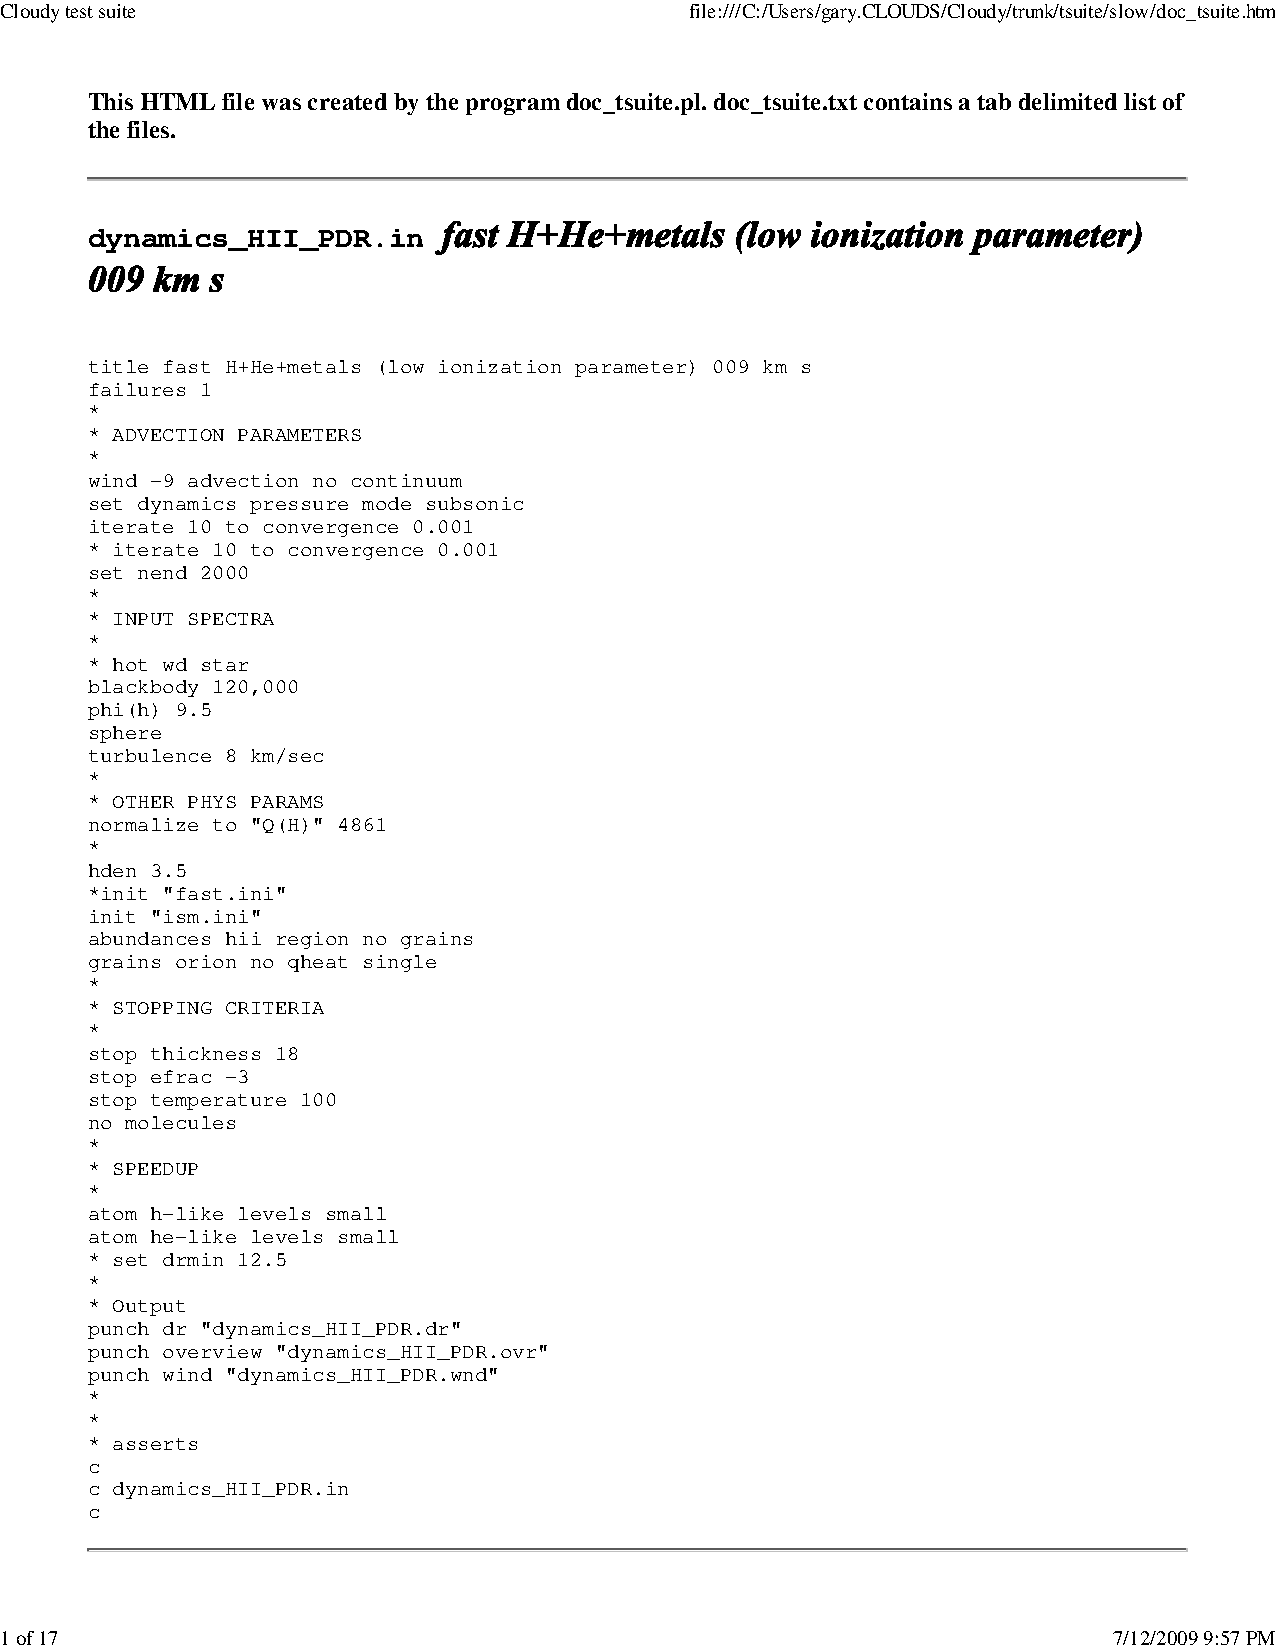
\includepdf[pages=-]{../../../tsuite/slow/doc_tsuite.pdf}


\section{Sample Programs} 

\backmatter
\bibliographystyle{plainnat}
\bibliography{../common/bibliography2}

\end{document}
